% ===========================================================================
% Relazione di progetto
% Sistemi di Calcolo Parallelo e Applicazioni - A.A. 2025/2026
% Prodotto matrice densa x multivettore  Y <- A X  in MPI + CUDA
%
% Compilazione:   latexmk -pdf main.tex      (oppure: ./compila.sh)
% ===========================================================================
\documentclass[11pt,a4paper,oneside]{report}

% ---------------------------------------------------------------------------
% Preambolo: pacchetti, stile, macro del progetto.
% Nessun pacchetto esotico: tutto quello che serve sta in una TeX Live standard.
% ---------------------------------------------------------------------------

\usepackage[utf8]{inputenc}
\usepackage[T1]{fontenc}
\IfFileExists{lmodern.sty}{\usepackage{lmodern}}{}
\usepackage[italian]{babel}
\usepackage{microtype}

% Tolleranza tipografica: i nomi di file in tt non si sillabano, e senza un po'
% di elasticita' finirebbero fuori dal margine.
\tolerance=1200
\emergencystretch=3em
\hbadness=10000

\usepackage[a4paper,top=2.6cm,bottom=2.6cm,left=2.7cm,right=2.7cm]{geometry}
\usepackage{amsmath,amssymb}
\usepackage{graphicx}
\usepackage{xcolor}
\usepackage{booktabs}
\usepackage{multirow}
\usepackage{array}
\usepackage{longtable}
\usepackage{enumitem}
\usepackage{float}
\usepackage[font=small,labelfont=bf]{caption}
\usepackage{subcaption}
\usepackage{fancyhdr}
\usepackage{listings}
\usepackage{tcolorbox}
\usepackage{siunitx}
\usepackage{pgfplots}
\pgfplotsset{compat=1.16}
\usepackage{pgfplotstable}
\usepackage[hidelinks]{hyperref}
\usepackage[italian]{cleveref}

% ---------------------------------------------------------------------------
% Unita' di misura
% ---------------------------------------------------------------------------
\sisetup{
  detect-weight       = true,
  detect-family       = true,
  group-digits        = integer,
  group-minimum-digits= 4,
  output-decimal-marker = {,},
  per-mode            = symbol
}
\DeclareSIUnit{\flop}{FLOP}
\DeclareSIUnit{\gflops}{GFLOPS}
\DeclareSIUnit{\gib}{GiB}
\DeclareSIUnit{\mib}{MiB}
\DeclareSIUnit{\kib}{KiB}

% ---------------------------------------------------------------------------
% Intestazioni
% ---------------------------------------------------------------------------
\pagestyle{fancy}
\fancyhf{}
\fancyhead[L]{\small\nouppercase{\leftmark}}
\fancyhead[R]{\small\thepage}
\renewcommand{\headrulewidth}{0.4pt}

% ---------------------------------------------------------------------------
% Notazione ricorrente del progetto
% ---------------------------------------------------------------------------
\newcommand{\Mat}[1]{\ensuremath{#1}}
\newcommand{\mloc}{\ensuremath{m_{\text{loc}}}}
\newcommand{\nloc}{\ensuremath{n_{\text{loc}}}}
\newcommand{\Prow}{\ensuremath{P_r}}
\newcommand{\Pcol}{\ensuremath{P_c}}
\newcommand{\Ai}{\ensuremath{I}}                  % intensita' aritmetica
\newcommand{\code}[1]{\texttt{#1}}
\newcommand{\file}[1]{\texttt{#1}}
\newcommand{\kernelname}[1]{\texttt{#1}}

% ---------------------------------------------------------------------------
% Marcatori dei dati ancora da raccogliere.
%
% Sono volutamente VISIBILI: questa relazione viene compilata mentre le
% campagne sono in corso, e un segnaposto che non si vede e' un segnaposto che
% finisce in consegna. Per la versione finale basta commentare la riga
% \todovisibiletrue qui sotto: i marcatori spariscono dal PDF e restano nel
% sorgente.
% ---------------------------------------------------------------------------
\newif\iftodovisibile
\todovisibiletrue          % <-- commentare questa riga per la consegna finale

\definecolor{todorosso}{HTML}{B3261E}
\definecolor{todogiallo}{HTML}{FFF4E5}
\definecolor{grigiodato}{HTML}{9E9E9E}

% Nota a margine da risolvere
\newcommand{\TODO}[1]{%
  \iftodovisibile
    \textcolor{todorosso}{\textbf{[DA FARE: #1]}}%
  \fi
}

% Singolo numero non ancora misurato, dentro una tabella
\newcommand{\dato}{\textcolor{grigiodato}{--}}

% Blocco di testo che dipende da misure non ancora disponibili
\newenvironment{daverificare}
  {\begin{tcolorbox}[colback=todogiallo,colframe=todorosso,boxrule=0.5pt,
                     left=6pt,right=6pt,top=4pt,bottom=4pt,
                     title=\small\textbf{Da completare con i dati della campagna}]}
  {\end{tcolorbox}}

% Ipotesi interpretativa non ancora confermata da un profilo
\newenvironment{ipotesi}[1]
  {\begin{tcolorbox}[colback=blue!3,colframe=blue!35,boxrule=0.5pt,
                     left=6pt,right=6pt,top=4pt,bottom=4pt,
                     title=\small\textbf{Ipotesi: #1}]}
  {\end{tcolorbox}}

% Segnaposto grafico: riquadro delle dimensioni della figura definitiva
\newcommand{\figuradafare}[2][0.72\linewidth]{%
  \begin{tcolorbox}[colback=todogiallo,colframe=todorosso,boxrule=0.6pt,
                    width=#1,halign=center,valign=center,height=5.2cm]
    \textcolor{todorosso}{\textbf{Figura da generare}}\\[2pt]
    \small #2
  \end{tcolorbox}%
}

% ---------------------------------------------------------------------------
% Listati
% ---------------------------------------------------------------------------
\definecolor{codegrigio}{HTML}{F5F5F5}
\definecolor{codecommento}{HTML}{4C7A34}
\definecolor{codekeyword}{HTML}{1A4F9C}

\lstdefinestyle{scpa}{
  backgroundcolor=\color{codegrigio},
  basicstyle=\ttfamily\footnotesize,
  keywordstyle=\color{codekeyword}\bfseries,
  commentstyle=\color{codecommento}\itshape,
  stringstyle=\color{todorosso},
  numbers=none,
  frame=single,
  framesep=4pt,
  rulecolor=\color{black!25},
  breaklines=true,
  breakatwhitespace=true,
  showstringspaces=false,
  columns=fullflexible,
  keepspaces=true,
  captionpos=b,
  aboveskip=1.0em,
  belowskip=1.0em,
  literate={à}{{\`a}}1 {è}{{\`e}}1 {é}{{\'e}}1 {ì}{{\`i}}1
           {ò}{{\`o}}1 {ù}{{\`u}}1 {°}{{$^\circ$}}1
}
\lstset{style=scpa}
\lstdefinelanguage{cuda}[ANSI]{C++}{
  morekeywords={__global__,__device__,__shared__,__restrict__,__syncthreads,
                __shfl_down_sync,blockIdx,threadIdx,blockDim,cudaMalloc,
                cudaMemcpy,cudaEventRecord,scalar_t}
}
\lstdefinelanguage{shell}{
  morekeywords={make,mpirun,nvcc,module,ompi_info,nsys,ncu,nvidia-smi},
  sensitive=true,
  morecomment=[l]{\#}
}
\renewcommand{\lstlistingname}{Listato}

% ---------------------------------------------------------------------------
% Stile comune dei grafici
% ---------------------------------------------------------------------------
\pgfplotsset{
  scpa/.style={
    width=0.78\linewidth,
    height=6cm,
    grid=both,
    grid style={line width=.1pt, draw=black!12},
    major grid style={line width=.2pt,draw=black!30},
    tick align=outside,
    legend cell align=left,
    legend style={font=\footnotesize,draw=black!25},
    label style={font=\small},
    tick label style={font=\footnotesize},
    every axis plot/.append style={line width=1pt, mark size=2pt}
  }
}


% --- Dati di testata ------------------------------------------------------
\newcommand{\titolorelazione}{Prodotto matrice densa per multivettore\\ in MPI e CUDA}
\newcommand{\sottotitolorelazione}{Progetto di fine corso}
\newcommand{\corso}{Sistemi di Calcolo Parallelo e Applicazioni}
\newcommand{\annoaccademico}{A.A. 2025/2026}
\newcommand{\autoreuno}{Alessandro Vassallo}
\newcommand{\matricolauno}{0366572}
\newcommand{\autoredue}{Andrea Galluzzi}
\newcommand{\matricoladue}{0365026}
\newcommand{\repository}{https://github.com/AleVassa00/parallel-computing-project}

\begin{document}

\begin{titlepage}
\centering
\thispagestyle{empty}

\vspace*{1.2cm}

{\large\scshape Universit\`a degli Studi di Roma ``Tor Vergata''\par}
\vspace{0.3cm}
{\normalsize Macroarea di Ingegneria \\ Corso di Laurea Magistrale in Ingegneria Informatica\par}

\vspace{2.0cm}

\rule{\linewidth}{0.5pt}\\[0.6cm]
{\LARGE\bfseries \titolorelazione \par}
\vspace{0.5cm}
{\large \sottotitolorelazione \par}
\rule{\linewidth}{0.5pt}

\vspace{1.6cm}

{\large \corso \\ \annoaccademico \par}

\vspace{2.4cm}

\begin{minipage}{0.46\textwidth}
  \centering
  {\small\itshape Autori}\\[4pt]
  \autoreuno\\{\small\matricolauno}\\[8pt]
  \autoredue\\{\small\matricoladue}
\end{minipage}

\vfill

{\small Codice sorgente: \url{\repository}}\\[4pt]
{\small Versione della relazione del \today}

\iftodovisibile
\vspace{0.8cm}
\begin{tcolorbox}[colback=todogiallo,colframe=todorosso,boxrule=0.6pt,width=0.85\linewidth]
  \small\centering
  \textcolor{todorosso}{\textbf{Bozza di lavoro.}} I marcatori in rosso segnalano
  i punti che dipendono da campagne di misura non ancora concluse. Per la
  versione di consegna, commentare \code{\textbackslash todovisibiletrue} in
  \file{preambolo.tex}.
\end{tcolorbox}
\fi

\vspace{0.5cm}
\end{titlepage}
\cleardoublepage


\pagenumbering{roman}
\tableofcontents
\cleardoublepage
\pagenumbering{arabic}

\chapter{Introduzione}
\label{cap:introduzione}

\section{Obiettivo}

Il progetto realizza un nucleo di calcolo per il prodotto fra una matrice densa
e un multivettore,
\begin{equation}
  Y \leftarrow A X ,
  \qquad
  A \in \mathbb{R}^{M \times N},\quad
  X \in \mathbb{R}^{N \times k},\quad
  Y \in \mathbb{R}^{M \times k},
  \label{eq:problema}
\end{equation}
con $k$ \emph{piccolo}: il multivettore è una matrice densa alta e strettissima.
Il codice funziona per $k$ generico ed è collaudato sui cinque valori richiesti
dalla traccia, $k \in \{3, 6, 8, 20, 32\}$.

\medskip

La parallelizzazione è ibrida a due livelli:

\begin{itemize}
  \item \textbf{MPI (Message Passing Interface)} costituisce il livello esterno, responsabile della distribuzione dei dati su una griglia di processi bidimensionale e della comunicazione fra processi
  \item la parallelizzazione interna al singolo processo è affidata a \textbf{CUDA (Compute Unified Device Architecture)},
  che costituisce il backend di accelerazione su GPU NVIDIA.
\end{itemize}
I due livelli non sono alternativi ma sovrapposti: ogni processo
MPI possiede un blocco di $A$ e delega il calcolo del proprio contributo
parziale a un \emph{backend} locale, che può essere un kernel CUDA oppure un nucleo di CPU.
\chapter{Il kernel di calcolo}
\label{cap:problema}

Questo capitolo fissa tre cose che il resto della relazione dà per acquisite:
che cosa il nucleo calcola e come se ne contano le operazioni, in che ordine
conviene scandire i tre cicli, e da dove vengono i dati. Sono scelte fatte una
volta sola, prima di qualunque backend: i capitoli su MPI, CPU e CUDA le
ereditano senza rimetterle in discussione.

\section{Che cosa calcola il nucleo}
\label{sec:definizione}

Il nucleo calcola $Y \leftarrow A X$, con $A$ densa $M \times N$ e $X$
multivettore $N \times k$. Elemento per elemento:
\begin{equation}
  Y[i][c] \;=\; \sum_{j=0}^{N-1} A[i][j]\, X[j][c],
  \qquad 0 \le i < M,\ 0 \le c < k .
  \label{eq:definizione}
\end{equation}

La traccia fissa i gradi di libertà: $M$ ed $N$ sono scelte dall'utente a
runtime, $k$ deve funzionare per valore \emph{generico} e il collaudo deve
coprire almeno $k = 3,\ 6,\ 8,\ 20,\ 32$. Il progetto rispetta entrambe le
richieste, ma con una distinzione che conviene anticipare subito: sui cinque
$k$ del collaudo il nucleo di CPU usa funzioni specializzate a tempo di
compilazione, mentre ogni altro $k$ passa da un percorso generico con
prestazioni diverse (\cref{cap:kernel-cpu}).

\subsection{Conteggio delle operazioni}

Il conteggio si costruisce in due passi.

\emph{Passo 1 - un singolo elemento.} Ogni $Y[i][c]$ è una somma di $N$
prodotti: servono $N$ moltiplicazioni e $N-1$ addizioni, ma la convenzione
standard, e quella imposta dalla traccia, arrotonda a $2$ FLOP per termine.

\emph{Passo 2 - tutta la matrice.} Gli elementi di $Y$ sono $M \cdot k$.

Quindi:
\begin{equation}
  \mathrm{FLOP}(M,N,k) = 2\,M\,N\,k ,
  \qquad
  \mathrm{GFLOPS} = \frac{2\,M\,N\,k}{T \cdot 10^{9}} .
  \label{eq:flops}
\end{equation}

Su questa formula la traccia impone tre vincoli, che vale la pena enunciare
qui perché condizionano tutta la metodologia di misura:

\begin{enumerate}[nosep,left=0pt]
  \item $T$ è il tempo \textbf{medio per invocazione}, ottenuto ripetendo il
        nucleo più volte sulla stessa matrice.
  \item In $T$ entra \textbf{solo il calcolo}: preprocessamento, I/O ed
        eventuali trasferimenti da e verso la scheda CUDA restano fuori. La
        traccia consente però di misurarli e discuterli a parte, ed è quello
        che il progetto fa. Che cosa esattamente venga cronometrato, e con
        quale orologio, è trattato in \cref{sec:metriche}.
  \item $M$ ed $N$ sono le dimensioni della matrice \textbf{globale}, anche
        quando l'esecuzione è distribuita. È proprio questo che
        rende leggibile lo speedup: il lavoro totale non cambia con il numero
        di processi, cambia solo $T$.
\end{enumerate}

\section{Come vengono memorizzati i dati}
\label{sec:layout}

Tutte e tre le matrici sono \textbf{row-major}: \emph{gli elementi di una stessa
riga sono adiacenti}.

La matrice $A$ ha inoltre una propria \emph{leading dimension} \code{lda}, cioè
la distanza in elementi fra l'inizio di una riga e l'inizio della successiva
nella rappresentazione in memoria.
La leading dimension è stata introdotta per permettere \emph{padding} fra righe consecutive
e per ricevere direttamente blocchi non contigui mediante datatype MPI derivati.
In realtà, le matrici X e Y la leading dimension è \emph{sempre} fissata a $k$,
che è il numero di colonne, e quindi le righe sono compatte.
La leading dimensione è sfruttata:
\[
  A[i][j] \;=\; \code{A\_loc}[\,i \cdot \code{lda} + j\,], \qquad
  X[j][c] \;=\; \code{X\_loc}[\,j \cdot \code{ldx} + c\,], \qquad
  Y[i][c] \;=\; \code{Y\_loc}[\,i \cdot \code{ldy} + c\,].
\]
Quando \code{lda} coincide con il numero di colonne il buffer è compatto;
quando è maggiore, fra una riga e l'altra restano delle celle inutilizzate, per l'appunto il \emph{padding}.

\paragraph{Perché \code{lda} è separata da \code{n\_loc}.}
Il blocco che un processo possiede è una sottomatrice di $A$, quindi
\textbf{non è contiguo nella matrice globale}: le sue righe sono distanti $N$
elementi l'una dall'altra. La distribuzione usa per questo un datatype
derivato \code{MPI\_Type\_vector}, con stride $N$ dal lato del mittente e
stride \code{lda} dal lato del ricevente, così il blocco viene depositato
direttamente nel buffer locale senza copie intermedie (\cref{cap:mpi}).
Tenere \code{lda} come parametro indipendente aggiunge a questo la possibilità
di avere padding fra le righe locali.s

\paragraph{Perché \code{ldx} e \code{ldy} invece sono fissate a $k$.}
L'interfaccia del kernel (\cref{app:interfaccia}) le espone e ogni backend le
onora, ma il driver distribuito impone $\code{ldx} = \code{ldy} = k$, cioè
buffer compatti. La ragione è nelle collettive: il \code{MPI\_Bcast} di $X$ e
il \code{MPI\_Reduce} di $Y$ lavorano con conteggi contigui, e descrivere uno
stride richiederebbe di costruire un datatype derivato a ogni invocazione,
\emph{dentro} la regione cronometrata. $A$ invece non attraversa nessuna
collettiva, ed è per questo che è l'unica delle tre a potersi permettere il
padding.

Il fatto che le $k$ colonne di $X$ siano adiacenti in memoria non è un
dettaglio di comodo: è la proprietà su cui si regge tutta la
\cref{sec:schemi}.

\begin{ipotesi}{}
{Un backend CUDA prevede in alternativa una disposizione
\textbf{column-major} di $X$, ma come opzione di build e con effetti discussi al
momento giusto (\cref{cap:kernel-cuda}); il default, e tutto ciò che segue, è
row-major.}
\end{ipotesi}

\section{Ordine dei cicli: schema A contro schema B}
\label{sec:schemi}

La \cref{eq:definizione} contiene tre indici, $i$, $j$ e $c$.
Indipendentemente dall'ordine in cui viene
scelto di scandire gli indici, l'operazione produce lo stesso risultato,
ma il diverso ordine con il quale vengono scanditi non danno affatto le stesse prestazioni.
È il primo punto in cui il progetto si
allontana da una trascrizione letterale della definizione.

\subsection{Gli schemi candidati}

I due candidati sono:

\begin{center}
\begin{minipage}[t]{0.47\linewidth}
\textbf{Schema A} ($i \to j \to c$)
\begin{lstlisting}[language=C]
for i:
  acc[0..k) = 0
  for j:
    a = A[i][j]
    for c:
      acc[c] += a * X[j][c]
  Y[i][0..k) = acc[0..k)
\end{lstlisting}
\end{minipage}\hfill
\begin{minipage}[t]{0.47\linewidth}
\textbf{Schema B} ($i \to c \to j$)
\begin{lstlisting}[language=C]
for i:
  for c:
    s = 0
    for j:
      s += A[i][j] * X[j][c]
    Y[i][c] = s
\end{lstlisting}
\end{minipage}
\end{center}

Lo schema~B è la trascrizione letterale della definizione, ed è esattamente
l'esecuzione di $k$ prodotti matrice-vettore indipendenti, uno per colonna.
Lo schema~A scambia i due cicli interni, cambiando anche il ``ruolo'' della matrice $A$.

Si segua una singola riga $i$.

\emph{Schema B.} Il ciclo su $c$ sta fuori e quello su $j$ dentro, quindi per
ogni colonna $c$ il ciclo interno percorre l'intera riga
$A[i][0 \ldots N{-}1]$. Finita una colonna si ricomincia da capo con la
successiva, sulle stesse celle. La riga viene dunque letta $k$ volte, per un
totale di $kN$ letture di $A$ a fronte delle $N$ celle che la riga contiene.

\emph{Schema A.} Il ciclo su $j$ sta fuori e quello su $c$ dentro. Il valore
$a = A[i][j]$ viene letto una volta sola e consumato subito da tutti e $k$ gli
accumulatori, con gli aggiornamenti
$\code{acc}[c] \mathrel{+}= a \cdot X[j][c]$ per $c = 0 \ldots k-1$; poi si
passa a $j+1$ e quel valore di $A$ non serve più. La riga viene letta una volta
sola, per un totale di $N$ letture. Il riuso di $A$ vale quindi esattamente
$k$, e vale per costruzione: non dipende dalla taglia del problema né da
condizioni sul valore di $k$.

Perché il risparmio sia reale gli accumulatori devono stare in registro, e
perché il compilatore possa tenerceli deve conoscerne il numero a tempo di
compilazione: è il motivo delle specializzazioni su $k$ descritte in
\cref{sec:specializzazione}.

Si potrebbe obiettare che le riletture dello schema~B le assorbe la cache, e in
parte è così, ma solo finché la dimensione della riga è contenibile nella cache.
Una riga di $A$ occupa $N s$
byte, dove  $s$ è la dimensione in byte di ogni elemento della matrice
e $N$ è la dimensione che la traccia chiede di far crescere: il caso
interessante è proprio quello in cui la riga eccede i livelli di cache vicini
al calcolo o, sulla GPU, quello in cui la riga eccede la shared memory di un blocco. Il modello che segue
conta perciò il traffico verso la memoria principale, che è il livello che
finisce per determinare il tempo.

\subsection{La quantificazione: intensità aritmetica}

L'\emph{intensità aritmetica} $\Ai$ è il rapporto fra i FLOP eseguiti e i byte
che attraversano il livello di memoria considerato. Detta $s$ la dimensione in
byte dello scalare, e contando il solo traffico su $A$ come giustificato in
\cref{sec:traffico}:

\begin{equation}
  \Ai_{\text{A}} \;=\; \frac{2\,M N k}{M N s} \;=\; \frac{2k}{s},
  \qquad
  \Ai_{\text{B}} \;=\; \frac{2\,M N k}{k\,M N s} \;=\; \frac{2}{s} .
  \label{eq:intensita}
\end{equation}

Il numeratore è lo stesso: i FLOP da fare sono fissati dal problema. Cambia il
denominatore, perché lo schema~B legge gli $MN$ elementi di $A$ una volta per
ciascuna delle $k$ colonne.

In FP64 ($s = 8$) questo significa $\Ai_{\text{A}} = k/4$ contro
$\Ai_{\text{B}} = 1/4$ \si{\flop\per\byte}: lo schema~A guadagna esattamente
un fattore $k$, e a $k = 32$ porta l'intensità da $0{,}25$ a
\SI{8}{\flop\per\byte}. 

È questo salto che sposta il nucleo da un regime saldamente memory-bound a un
regime in cui, sulla GPU in doppia precisione, il limite può diventare il
calcolo. La discussione quantitativa, con i picchi reali della scheda, è nel
\cref{cap:roofline}.

\subsection{Un limite che non si può superare}

$\Ai_{\text{A}} = 2k/s$ è il \textbf{massimo} ottenibile: gli $MN$ elementi di
$A$ vanno letti almeno una volta e i FLOP sono fissati, quindi nessuna
riorganizzazione ulteriore può migliorare il rapporto. Tutto il lavoro di
ottimizzazione successivo, su CPU come su GPU, riguarda allora il traffico su
$X$ e la capacità di tenere i $k$ accumulatori in registro, non l'intensità
rispetto ad $A$, che è già al suo limite.

Con un'eccezione, che la traccia rende rilevante chiedendo $k$ generico. Tenere
$k$ accumulatori in registro è possibile finché $k$ è abbastanza piccolo: oltre
una certa ampiezza il nucleo di CPU blocca le colonne a gruppi di
$\code{KB} = 32$ e rilegge $A$ una volta per gruppo, cosicché in generale
\[
  \Ai_{\text{A}}(k) \;=\; \frac{2k}{s \cdot \lceil k/\code{KB} \rceil}.
\]
Per i cinque $k$ del collaudo il ciclo sui blocchi è degenere, $A$ viene letta
una volta sola e si ricade nella \cref{eq:intensita}; per $k = 64$ i passaggi
sono due e l'intensità si ferma al valore che aveva a $k = 32$. Il dettaglio,
con il microbenchmark che lo misura, è in \cref{sec:specializzazione}.

\subsection{Una proprietà che conta sull'hardware reale}

Nello schema~A entrambi i flussi di lettura sono a \textbf{passo unitario}. La
riga di $A$ è contigua per costruzione e la riga di $X$ lo è perché $X$ è
row-major con le $k$ colonne adiacenti (\cref{sec:layout}). Nessuno dei due
accessi ha stride, quindi i prefetcher hardware lavorano nelle condizioni
migliori e, sulla GPU, gli accessi delle lane di uno stesso warp sono
coalescibili. Lo schema~B, per ottenere la stessa proprietà sull'accesso a
$X$, richiederebbe $X$ column-major, cioè un layout diverso da quello che
serve altrove.

\section{Precisione}
\label{sec:precisione}

Tutto il codice usa un unico tipo \code{scalar\_t}, definito in
\file{src/common/scalar.h}, che vale \code{double} per default e \code{float}
compilando con \code{PREC=float} (il Makefile traduce la variabile nella macro
\code{-DUSE\_FLOAT}). Anche il tipo MPI segue lo scalare, attraverso la macro
\code{SCALAR\_MPI\_TYPE}, così le collettive non vanno toccate.

Il confronto FP64/FP32 è quindi un flag di compilazione e non una seconda
copia dei sorgenti: le due build eseguono esattamente lo stesso codice, che è
la sola condizione in cui il confronto misura la precisione e non due
implementazioni diverse.

\paragraph{Effetto sul modello roofline.} La scelta della precisione non è
neutra, e agisce in \textbf{due modi opposti}:

\begin{itemize}[nosep,left=0pt]
  \item dimezzando $s$ la \cref{eq:intensita} \emph{raddoppia} l'intensità
        aritmetica, da $k/4$ a $k/2$. Da solo, questo avvicinerebbe il nucleo
        al regime compute-bound;
  \item ma il punto di crossover del roofline vale $P_{\text{picco}}/B$, e su
        una GPU Turing il picco FP32 è $32$ volte il picco FP64. Il crossover
        si sposta quindi a destra di un fattore $32$.
\end{itemize}

Il secondo effetto è $16$ volte più forte del primo e prevale nettamente: in
singola precisione il nucleo finisce \textbf{saldamente memory-bound} su tutto
l'intervallo di $k$ della traccia, mentre in doppia precisione è
compute-bound già da $k = 6$. I due regimi sono qualitativamente diversi, ed è
questo il vero argomento con cui il progetto discute la precisione: la doppia
non costa il fattore $2$ del traffico, costa il fattore $32$ del picco. I
numeri sono in \cref{sec:roofline-gpu}.

\paragraph{Effetto sulla validazione.} \file{scalar.h} deriva dal tipo anche
\code{SCALAR\_EPS} e la tolleranza del confronto con l'oracolo seriale, che
non è una costante ma cresce con la lunghezza della riduzione. Il modello e la
costante misurata sono discussi in \cref{cap:validazione}.

\section{Generazione riproducibile dei dati}
\label{sec:generazione}

Le matrici di test sono generate, non lette da file. La traccia lo consente
esplicitamente, elencando la generazione fra le strategie di collaudo, e in
cambio chiede che sia \textbf{ripetibile}.

\subsection{Il generatore}

Il generatore è \code{splitmix64}, un mixer a 64 bit \textbf{senza stato}. La
differenza rispetto a un generatore pseudocasuale ordinario è tutta qui: un
generatore con stato produce una \emph{sequenza}, e per ottenere l'elemento in
posizione $p$ bisogna averlo fatto avanzare $p$ volte. Un mixer stateless va
da $(\text{seed}, \text{chiave})$ al valore in un passo solo. La chiave scelta è
l'\textbf{indice lineare globale} dell'elemento:

\begin{equation}
  A[i][j] \;=\; g\bigl(\text{seed},\ \Sigma_A,\ i \cdot N + j \bigr),
  \qquad
  X[j][c] \;=\; g\bigl(\text{seed},\ \Sigma_X,\ j \cdot k + c \bigr),
  \label{eq:gen}
\end{equation}
dove $\Sigma_A$ e $\Sigma_X$ sono due identificatori di \emph{stream} distinti, che
servono a evitare che $A$ e $X$ abbiano lo stesso pattern di valori. Il seed
viene mescolato prima con lo stream e poi con la chiave: due passaggi, perché
uno solo lascerebbe correlati i valori di chiavi vicine. Dei $64$ bit
prodotti si usano i $53$ alti, che danno un \code{double} esatto in $[0,1)$,
riscalato poi in $[-1,1)$.

Il valore di un elemento dipende dunque \emph{solo} dalla sua posizione
globale: mai dal processo che lo calcola, mai dall'ordine in cui viene
generato, mai dalla forma della griglia.

\subsection{Le tre conseguenze, tutte usate dal progetto}

\begin{enumerate}[nosep,left=0pt]
  \item ogni processo può generare \textbf{direttamente} il proprio blocco
        locale, senza che una copia globale della matrice esista mai in
        memoria. È ciò che permette di misurare taglie che su un solo nodo non
        starebbero;
  \item la stessa matrice globale si ottiene con \emph{qualunque} griglia di
        processi e con qualunque modalità di inizializzazione. Due
        configurazioni diverse sono quindi confrontabili elemento per
        elemento;
  \item l'esecuzione seriale di \cref{cap:validazione}, usata come oracolo,
        può ricostruire da sé la
        porzione che gli serve, senza ricevere dati dagli altri processi.
\end{enumerate}

\subsection{Perché i valori hanno media nulla}

I valori sono distribuiti in $[-1, 1)$ a media nulla, e questa non è una scelta
estetica. Ogni elemento di $Y$ è una riduzione su $N$ termini, e l'errore di
arrotondamento di una riduzione dipende da come si compongono i segni: con
termini a media nulla gli arrotondamenti hanno segno indipendente e l'errore
cresce come $\varepsilon\sqrt{N}$, non come il pessimistico $\varepsilon N$
del caso in cui tutti i termini abbiano lo stesso segno. È questa proprietà
dei dati che rende possibile una tolleranza di validazione stretta invece di
una soglia fissa e generosa (\cref{cap:validazione}).

Una nota utile per il confronto fra precisioni: il generatore calcola sempre in
\code{double} e converte in \code{scalar\_t} solo alla fine. Le build FP64 e
FP32 lavorano quindi sugli stessi dati a meno del solo arrotondamento della
conversione, ed è la condizione che rende confrontabili i loro tempi.
\chapter{Architettura del software}
\label{cap:architettura}

\section{Moduli}

Il codice \`e diviso per responsabilit\`a, non per file: ogni cartella di
\file{src/} ha un compito unico e dipende solo da quelle sotto di s\'e.

\begin{table}[H]
\centering
\footnotesize
\caption{Struttura di \file{src/}.}
\label{tab:moduli}
\begin{tabular}{@{}p{0.20\linewidth}p{0.72\linewidth}@{}}
\toprule
\textbf{Modulo} & \textbf{Responsabilit\`a} \\
\midrule
\file{common/} & tipo scalare unico (\code{scalar\_t}), tolleranza di
  validazione, utility di terminazione e cronometro \\
\file{index/} & partizionamento a blocchi degli indici globali: dimensione,
  offset e proprietario di ogni blocco \\
\file{gen/} & generatore riproducibile senza stato (\cref{sec:generazione}) \\
\file{serial/} & implementazione seriale minimale, usata come oracolo \\
\file{kernel/} & \code{local\_gemm}: un file per implementazione, \code{.c} o
  \code{.cu}, tutte dietro la stessa interfaccia \\
\file{mpi/} & griglia cartesiana, layout dei blocchi, distribuzione dei dati,
  algoritmo distribuito $Y = AX$ \\
\file{bench/} & driver di misura e validazione, parsing delle opzioni, output CSV \\
\bottomrule
\end{tabular}
\end{table}

La dipendenza pi\`u importante \`e quella che \textbf{non} esiste: \file{mpi/} non
include mai un header di un backend specifico. Vede solo
\file{kernel/kernel.h}, e non ha modo di sapere se sotto giri lo schema~A
scalare o un kernel CUDA.

\section{L'interfaccia unica del kernel locale}
\label{sec:interfaccia}

Ogni backend implementa tre funzioni di esecuzione e un insieme di canali di
misura e di introspezione:

\begin{lstlisting}[language=C,caption={Interfaccia di \file{src/kernel/kernel.h}.}]
/* esecuzione */
local_gemm_t *local_gemm_create(int m, int n, int k,
                                const scalar_t *A_loc,
                                int lda, int ldx, int ldy);
void local_gemm(local_gemm_t *ctx,
                const scalar_t *RESTRICT X, int ldx,
                scalar_t *RESTRICT Y, int ldy);
void local_gemm_destroy(local_gemm_t *ctx);

/* tempi della singola invocazione */
double local_gemm_last_compute_seconds(const local_gemm_t *ctx);
double local_gemm_last_h2d_X_seconds(const local_gemm_t *ctx);
double local_gemm_last_d2h_Y_seconds(const local_gemm_t *ctx);

/* byte trasferiti, per trasformare i tempi in banda */
size_t local_gemm_bytes_h2d_A(const local_gemm_t *ctx);
size_t local_gemm_bytes_h2d_X_per_call(const local_gemm_t *ctx);
size_t local_gemm_bytes_d2h_Y_per_call(const local_gemm_t *ctx);

/* preparazione, totale e scomposta */
double local_gemm_setup_seconds(const local_gemm_t *ctx);
double local_gemm_setup_device_init_seconds(const local_gemm_t *ctx);
double local_gemm_setup_device_alloc_seconds(const local_gemm_t *ctx);
double local_gemm_setup_h2d_A_seconds(const local_gemm_t *ctx);

/* piano di esecuzione effettivamente scelto a runtime */
int local_gemm_blocks_per_sm(const local_gemm_t *ctx);
int local_gemm_x_rows_per_tile(const local_gemm_t *ctx);

const char *kernel_name(void);
\end{lstlisting}

I canali oltre i primi tre sono la parte che ha richiesto pi\`u lavoro, e la
ragione \`e in \cref{sec:metriche}: la traccia esclude dal tempo $T$ i
trasferimenti da e verso la scheda e il preprocessing, ma consente
esplicitamente di misurarli e discuterli a parte --- e per discuterli non basta
il totale, servono le singole voci. Tutti seguono la stessa convenzione: un
valore \textbf{negativo} (o $0$ per i byte) significa ``non applicabile a questo
backend'', ed \`e ci\`o che rende una riga di CPU riconoscibile a colpo d'occhio
in un CSV che contiene anche righe GPU.

Le ultime due funzioni non sono metriche di prestazione ma la
\emph{configurazione} scelta a runtime dal backend: senza di esse una campagna
sul tiling mostrerebbe curve che salgono e scendono senza poter dire se sia
cambiato il tile, l'occupancy, o entrambi (\cref{sec:piano-tile}).

La scelta del backend \`e del \code{Makefile} (variabile \code{KERNEL}), non del
codice: non esiste nessun \code{switch} a runtime fra implementazioni, e quindi
nessun costo n\'e nessuna possibilit\`a di misurare per sbaglio un percorso
diverso da quello che si crede.

\subsection{Perch\'e il ciclo di vita ha tre fasi}
\label{sec:tre-fasi}

La separazione fra \code{create}, \code{local\_gemm} e \code{destroy} \`e la
scelta architetturale con l'effetto pi\`u diretto sulle misure, e discende da una
asimmetria del problema:

\begin{center}
\emph{$A$ non cambia mai fra un'invocazione e l'altra; $X$ e $Y$ cambiano sempre.}
\end{center}

$X$ arriva da un \code{MPI\_Bcast} e $Y$ deve tornare a un \code{MPI\_Reduce},
quindi entrambe attraversano ogni invocazione. $A$, invece, viene generata (o
ricevuta) una volta sola e resta identica per tutte le repetition. Tutto ci\`o che
riguarda $A$ pu\`o dunque stare in \code{create}, che \`e preprocessing e non viene
cronometrato.

Per il backend di CPU questo \`e quasi vuoto: \code{create} registra forma e
puntatore. Per i backend CUDA \`e invece il punto in cui $A$ viene copiata in VRAM
\emph{una volta sola}. Il guadagno non \`e cosmetico: con $A$ dell'ordine dei
gigabyte, una \code{cudaMemcpy} H2D per invocazione misurerebbe la banda PCIe e
non la GPU. La traccia consente esplicitamente di escludere dal tempo $T$ i
trasferimenti da e verso la scheda, e l'architettura rende questa esclusione una
propriet\`a strutturale invece che una sottrazione a posteriori.

Nella stessa fase vengono allocati anche i buffer di $X$ e $Y$ sul device e viene
eseguita una \code{cudaDeviceSynchronize} finale. La conseguenza \`e che nessuna
allocazione, e nessuna coda residua della copia di $A$, pu\`o cadere dentro la
prima repetition, neppure con \code{--warmup 0}.

\subsection{Lo stato in un contesto opaco}

Lo stato del backend vive in una \code{struct local\_gemm\_context} opaca, non in
variabili statiche di modulo. Il tipo \`e dichiarato in \file{kernel.h} e definito
in ciascun \code{.c}/\code{.cu}, quindi ogni backend gli d\`a i campi che gli
servono: il backend di CPU tiene forma e puntatore ad $A$, i backend CUDA
tengono i tre puntatori device, i due \code{cudaEvent} e i tempi.

Tre conseguenze pratiche: \`e esplicito nel tipo chi possiede la copia di $A$;
non esiste inizializzazione globale nascosta; il backend resta riutilizzabile,
perch\'e nulla vieta di avere pi\`u contesti vivi contemporaneamente.

\subsection{Compatibilit\`a C / C++ e il test che la difende}

I file \code{.cu} sono compilati da \code{nvcc} come C++, mentre il resto del
progetto \`e C11 compilato da \code{mpicc}. Due differenze toccano proprio
l'header condiviso: \code{restrict} non \`e una parola chiave del C++
(si scrive \code{\_\_restrict\_\_}) e i nomi delle funzioni C++ vengono decorati,
quindi senza \code{extern "C"} un backend \code{.cu} compilerebbe ma non
linkerebbe.

Entrambe le protezioni sono nell'header. La parte interessante \`e che la
propriet\`a \`e \emph{verificata}, e in due modi: il target \code{make check-cxx}
compila una sonda C++ che include \file{kernel.h} e \file{util.h}, e poi
controlla con \code{nm} che ognuno dei simboli dell'interfaccia --- tutte e
sedici le funzioni del listato precedente, pi\`u \code{xmalloc} e \code{die} ---
compaia \emph{non decorato} fra gli indefiniti dell'oggetto prodotto. Un
\code{extern "C"} dimenticato su una funzione aggiunta in seguito fallisce
quindi qui, su qualunque macchina e anche senza \code{nvcc}, e non come errore
di link sul server il giorno della campagna.

\section{Il driver di misura}

\file{src/bench/main.c} \`e l'unico punto che conosce sia MPI sia il kernel sia
le metriche. Fa, nell'ordine:

\begin{enumerate}[nosep,left=0pt]
  \item parsing e validazione delle opzioni (\cref{app:cli});
  \item creazione della griglia cartesiana e calcolo del layout locale;
  \item generazione o distribuzione di $A$ e $X$, e conversione del layout di
        $X$ se la build lo richiede --- ogni fase cronometrata separatamente
        (\cref{sec:tempi-esclusi});
  \item \code{local\_gemm\_create} (preprocessing del backend);
  \item \code{--warmup} invocazioni non cronometrate;
  \item \code{--reps} invocazioni cronometrate, con i tempi delle tre fasi
        raccolti per ogni repetition;
  \item riduzione dei tempi fra i rank, calcolo di media, mediana, minimo,
        deviazione standard e coefficiente di variazione;
  \item validazione opzionale contro l'oracolo seriale (\code{--check});
  \item stampa leggibile oppure riga CSV.
\end{enumerate}

Il fatto che warm-up e misura siano due cicli distinti sullo stesso codice, e non
un ciclo unico con i primi giri scartati a posteriori, \`e voluto: le
repetition cronometrate non contengono nessun ramo che le distingua dalle altre.

\section{Build: una configurazione, un binario}
\label{sec:build}

Ogni scostamento dalla configurazione di default produce un binario con un nome
proprio, come mostrato in \cref{tab:binari}. Non esiste un solo
\file{bin/matmul\_mpi} riscritto a ogni \code{make}.

\begin{table}[H]
\centering
\footnotesize
\caption{Corrispondenza fra configurazione di build e binario prodotto.}
\label{tab:binari}
\begin{tabular}{@{}p{0.46\linewidth}p{0.46\linewidth}@{}}
\toprule
\textbf{Comando} & \textbf{Binario} \\
\midrule
\code{make} & \file{bin/matmul\_mpi} \\
\code{make PREC=float} & \file{bin/matmul\_mpi-float} \\
\code{make FORCE\_GENERIC\_K=1} & \file{bin/matmul\_mpi-generic} \\
\code{make TEST\_A\_PADDING=8} & \file{bin/matmul\_mpi-pad8} \\
\code{make KERNEL=cuda\_naive} & \file{bin/matmul\_mpi-cuda\_naive} \\
\code{make KERNEL=cuda\_warp} & \file{bin/matmul\_mpi-cuda\_warp} \\
\code{make KERNEL=cuda\_warp\_smem} & \file{bin/matmul\_mpi-cuda\_warp\_smem} \\
\code{make KERNEL=cuda\_warp\_smem SMEM\_PAD=0} & \file{bin/matmul\_mpi-cuda\_warp\_smem-smempad0} \\
\code{make KERNEL=cuda\_warp\_smem TILE\_GRANULARITY=8} & \file{bin/matmul\_mpi-cuda\_warp\_smem-g8} \\
\code{make KERNEL=cuda\_warp\_smem SMEM\_BUDGET\_BYTES=16384} & \file{bin/matmul\_mpi-cuda\_warp\_smem-bud16384} \\
\code{make KERNEL=cuda\_warp\_tiled WARP\_COL\_TILE=4} & \file{bin/matmul\_mpi-cuda\_warp\_tiled-tile4} \\
\code{make KERNEL=cuda\_warp X\_LAYOUT=column} & \file{bin/matmul\_mpi-cuda\_warp-xcol} \\
\code{make BLOCK=512 KERNEL=cuda\_warp} & \file{bin/matmul\_mpi-cuda\_warp-blk512} \\
\code{make KERNEL=cublas} & \file{bin/matmul\_mpi-cublas} \\
\bottomrule
\end{tabular}
\end{table}

I parametri che entrano nel nome sono solo quelli che il backend selezionato
legge davvero: \code{TILE\_GRANULARITY} e \code{SMEM\_BUDGET\_BYTES} compaiono
soltanto con \kernelname{cuda\_warp\_smem}, \code{WARP\_COL\_TILE} soltanto con
\kernelname{cuda\_warp\_tiled}. Altrimenti si otterrebbero binari con nomi
diversi e contenuto identico, indistinguibili nel CSV perch\'e
\code{kernel\_name()} non cambierebbe. Anche gli oggetti sono per
configurazione (\file{obj/matmul\_mpi<config>/}), quindi cambiare precisione o
backend non pu\`o riutilizzare per sbaglio una compilazione precedente.

Il motivo \`e sperimentale, non organizzativo: una build non pu\`o sovrascriverne
un'altra e far misurare in singola precisione una campagna che si credeva in
doppia. Nello stesso spirito, \code{kernel\_name()} riporta nel CSV anche i
parametri che cambiano il codice generato --- per esempio
\code{cuda\_warp\_tiled(tile8)} oppure il suffisso \code{(blk512)} quando la
dimensione del blocco non \`e quella di default --- cos\`i le righe di uno sweep
restano distinguibili anche a distanza di settimane.

Il \code{Makefile} riconosce da s\'e se il backend richiesto \`e C o CUDA: se
esiste \file{src/kernel/<nome>.cu} lo compila con \code{nvcc -arch=sm\_75} e
linka \code{-lcudart} (e \code{-lcublas} per il backend cuBLAS). Su una macchina
priva di \code{nvcc} la build CUDA si ferma con un messaggio esplicito, mentre
tutto il resto del progetto continua a compilare: \`e la propriet\`a che ha
permesso di sviluppare su una macchina ARM64 senza GPU e misurare sul server.

\chapter{Parallelizzazione MPI}\label{cap:mpi}

Fino a questo punto il prodotto è stato descritto come se avvenisse dentro un
unico spazio di memoria: i cicli di \cref{sec:schemi} leggono $A$ e $X$ e
scrivono $Y$ come se tutte e tre fossero lì, a disposizione. Questo capitolo
rimuove quell'ipotesi. Il problema diventa far collaborare più processi che
non condividono niente, e le scelte che ne derivano condizionano tutto il
resto della relazione: la forma dei blocchi, che cosa viene cronometrato, e
perfino quali configurazioni ha senso misurare.

\section{Che cosa significa parallelizzare in MPI}\label{sec:mpi-intro}

MPI (\emph{Message Passing Interface}) è uno standard per programmare macchine
a \textbf{memoria distribuita}. Il modello di esecuzione è il seguente: lo
stesso programma viene avviato in $P$ copie, ciascuna un processo del sistema
operativo a sé stante, con il proprio spazio di indirizzi \textbf{privato}.
Nessun processo può leggere o scrivere una variabile di un altro. L'unico modo
perché un dato passi da un processo all'altro è che qualcuno lo invii
esplicitamente, con una chiamata di libreria, e qualcun altro lo riceva.

È una differenza sostanziale rispetto a un modello a memoria condivisa, dove i
thread vedono gli stessi indirizzi e la parallelizzazione consiste
essenzialmente nel ripartire le iterazioni di un ciclo. Qui ripartire le
iterazioni non basta, e non è nemmeno la prima cosa da decidere: prima bisogna
stabilire \textbf{chi possiede quale dato}. Da questa scelta discende tutto il
resto, perché un processo può calcolare solo ciò per cui possiede gli
ingredienti, e ogni ingrediente mancante è un messaggio da far viaggiare.

La parallelizzazione del nucleo si articola quindi in tre domande, in
quest'ordine:

\begin{enumerate}[nosep,left=0pt]
  \item \textbf{decomposizione} - come si tagliano $A$, $X$ e $Y$ fra i
        processi;
  \item \textbf{località} - quale parte del risultato ciascun processo riesce
        a calcolare con i soli dati che possiede;
  \item \textbf{comunicazione} - che cosa manca, e in quale direzione deve
        viaggiare perché il risultato locale diventi il risultato giusto.
\end{enumerate}

\begin{itemize}[nosep,left=0pt]
  \item Il \textbf{rank} è l'identificatore intero di un processo all'interno
        di un gruppo: è ciò che permette a un programma unico di comportarsi
        diversamente su processi diversi.
  \item Un \textbf{comunicatore} è un gruppo di processi assieme a un contesto
        di comunicazione isolato. Ogni operazione MPI avviene \emph{dentro} un
        comunicatore, e i rank hanno senso solo rispetto a quello:
        \code{MPI\_COMM\_WORLD} è il comunicatore predefinito che contiene
        tutti i processi, ma se ne possono costruire altri più piccoli, ed è
        esattamente ciò che il progetto fa.
  \item Un'operazione \textbf{collettiva} è un'operazione che tutti i processi
        di un comunicatore devono chiamare. Il progetto ne usa due:
        il \emph{broadcast}, in cui un processo possiede un dato e al termine
        lo possiedono tutti; e la \emph{reduce}, in cui ogni processo possiede
        un array della stessa forma, gli array vengono combinati elemento per
        elemento con un operatore associativo --- qui la somma --- e il
        risultato finisce su un solo processo.
  \item Il \textbf{root} è quel processo designato: la sorgente nel broadcast,
        il destinatario nella reduce.
\end{itemize}

\section{Perché si taglia \texorpdfstring{$A$}{A}, e perché in due direzioni}
\label{sec:perche-2d}

\subsection{Che cosa tagliare}

La prima decisione riguarda quale delle tre matrici vada distribuita. La
risposta viene da \cref{sec:traffico}: $A$ ha $MN$ elementi, $X$ e $Y$ ne
hanno rispettivamente $Nk$ e $Mk$, e con $k$ piccolo per definizione $A$ è più
grande delle altre due di un fattore che cresce con la taglia del problema.

Replicare $A$ su ogni processo sarebbe quindi la scelta peggiore possibile, e
per due ragioni indipendenti: ogni nodo dovrebbe contenerla per intero,
mettendo un tetto alla taglia massima trattabile a prescindere da quanti
processi si usino; e ogni processo la rileggerebbe tutta, quando è proprio il
traffico su $A$ a determinare il tempo. $A$ va dunque \textbf{tagliata}. $X$ e
$Y$, che sono piccole, possono invece permettersi di essere replicate lungo un
asse, e vedremo che è esattamente ciò che conviene fare.

\subsection{Come tagliare: due possibilità monodimensionali}

Tagliare $A$ significa assegnare a ogni processo una sottomatrice. Le
decomposizioni più semplici la tagliano lungo una sola dimensione, e la
\cref{eq:definizione} dice subito che cosa comportano.

\paragraph{Taglio a bande di righe.} Ogni processo possiede righe \emph{intere}
di $A$. Per calcolare $Y[i][c]$ serve tutta la riga $i$ di $A$ e tutte le
righe di $X$: un processo che possiede righe intere possiede quindi tutti i
fattori del primo tipo, ma gli serve $X$ per intero. Il vantaggio è che il
risultato che calcola è già \emph{definitivo}: nessuna somma finale fra
processi. Il costo è che $X$ deve essere replicata su tutti i $P$ processi.

\paragraph{Taglio a bande di colonne.} Ogni processo possiede colonne di $A$,
cioè, per ciascuna riga, solo una parte degli addendi della sommatoria. Gli
basta quindi la porzione di $X$ corrispondente alle proprie colonne --- $X$
viene tagliata e non replicata --- ma ciò che produce è un risultato
\textbf{parziale}, che riguarda tutte le righe di $Y$ e va sommato con i
parziali di tutti gli altri. La somma finale coinvolge $P$ processi su un
oggetto della taglia piena di $Y$.

\medskip

Le due alternative sono speculari: la prima paga la replicazione di $X$ su
tutti, la seconda la riduzione di $Y$ su tutti. In entrambe la comunicazione
coinvolge sempre l'intero insieme dei processi, e questo è il difetto
strutturale: aumentare $P$ non rende i messaggi più piccoli, li rende soltanto
più numerosi.

\subsection{Il taglio bidimensionale}

La terza possibilità taglia $A$ in entrambe le direzioni: ogni processo
possiede un \emph{rettangolo} della matrice. Le due necessità di prima
compaiono ora entrambe --- servono le righe di $X$ corrispondenti alle proprie
colonne di $A$, e il proprio contributo a $Y$ è parziale e va sommato --- ma
ciascuna coinvolge soltanto un \textbf{sottoinsieme} dei processi: quelli che
condividono le stesse colonne di $A$ per la prima, quelli che condividono le
stesse righe per la seconda. Nessuna delle due comunicazioni è più globale.

È questa la decomposizione richiesta dalla traccia, ed è quella che il progetto
implementa. Che sia effettivamente superiore alle due monodimensionali non è
però qualcosa da accettare sulla fiducia: è una proprietà quantificabile, e la
\cref{sec:modello-comunicazione} la dimostra con un modello di costo,
mostrando che le due decomposizioni 1D ne sono i casi degeneri. Il confronto
viene poi misurato direttamente in \cref{cap:risultati}.


% ---------------------------------------------------------------------------
% Figura: taglio bidimensionale di A, con X e Y tagliate lungo una sola
% dimensione. Da inserire in sezioni/04-mpi.tex, in \cref{sec:perche-2d}.
% ---------------------------------------------------------------------------
\begin{figure}[H]
\centering
\begin{tikzpicture}[scale=0.95,every node/.style={font=\footnotesize}]

  % --- A: griglia 2 x 3 di blocchi -----------------------------------------
  \foreach \r in {0,1} {
    \foreach \c in {0,1,2} {
      \draw[fill=black!4] (\c*1.7,-\r*1.7) rectangle ++(1.7,1.7);
      \node at (\c*1.7+0.85,-\r*1.7+0.85) {$(\r,\c)$};
    }
  }
  % etichette di riga e colonna della griglia
  \node[anchor=east] at (-0.15,0.85)  {riga 0};
  \node[anchor=east] at (-0.15,-0.85) {riga 1};
  \node at (0.85,1.95) {col.\ 0};
  \node at (2.55,1.95) {col.\ 1};
  \node at (4.25,1.95) {col.\ 2};
  \node at (2.55,-2.3) {$A$: tagliata in \emph{entrambe} le direzioni};

  % --- X: tagliata per bande di righe, una per banda di colonne di A -------
  \foreach \b in {0,1,2} {
    \draw[fill=black!8] (6.1,1.7-\b*1.133) rectangle ++(0.8,-1.133);
    \node at (6.5,1.7-\b*1.133-0.567) {$X_{\b}$};
  }
  \node[align=center] at (6.5,-2.3) {$X$\\segue\\le colonne};

  % --- Y: tagliata per bande di righe, una per banda di righe di A ---------
  \foreach \b in {0,1} {
    \draw[fill=black!8] (8.0,1.7-\b*1.7) rectangle ++(0.8,-1.7);
    \node at (8.4,1.7-\b*1.7-0.85) {$Y_{\b}$};
  }
  \node[align=center] at (8.4,-2.3) {$Y$\\segue\\le righe};

\end{tikzpicture}
\caption{Decomposizione dei dati su una griglia $2 \times 3$. Ogni processo
possiede un \emph{rettangolo} di $A$, individuato dalle sue coordinate nella
griglia. Il multivettore $X$ \`e tagliato per bande di righe, una per ciascuna
banda di colonne di $A$; $Y$ per bande di righe, una per ciascuna banda di
righe di $A$. Nessuna delle due \`e mai tagliata lungo $k$.}
\label{fig:taglio-2d}
\end{figure}

\subsection{Perché i processi vengono organizzati a griglia}

Resta un ultimo passaggio, che è di comodità ma non solo. Se il taglio del
dato è bidimensionale, conviene che lo sia anche il modo in cui si identificano
i processi: un processo individuato da una coppia di coordinate
$(r, c)$ invece che da un intero rende immediate le due relazioni che servono
di continuo. «I processi che possiedono le stesse colonne di $A$» diventa «i
processi della stessa colonna della griglia», e non un calcolo aritmetico sui
rank da rifare ogni volta.

MPI offre questa struttura nativamente, sotto il nome di \textbf{topologia
virtuale cartesiana}. È virtuale nel senso che non descrive come i nodi sono
fisicamente cablati: descrive come il programma vuole \emph{pensare}
all'insieme dei propri processi, lasciando però all'implementazione la
possibilità di sfruttare quell'informazione per disporli meglio sulla macchina
reale.

\section{Decomposizione a griglia bidimensionale}
\label{sec:griglia}

I $P$ processi vengono organizzati in una griglia cartesiana
$\Prow \times \Pcol = P$, costruita con \code{MPI\_Cart\_create}. La chiamata
restituisce un nuovo comunicatore nel quale ogni processo ha, oltre al proprio
rank, una coppia di coordinate recuperabile con \code{MPI\_Cart\_coords}: sono
le $(r,c)$ della sezione precedente, ed è su di esse che il codice ragiona da
qui in avanti.

Due parametri della chiamata meritano una nota:

\begin{itemize}[nosep,left=0pt]
  \item la griglia è dichiarata \textbf{non periodica}. La periodicità serve
        agli schemi in cui ogni processo comunica con i propri vicini e il
        bordo deve richiudersi sul lato opposto; qui le comunicazioni sono
        collettive lungo un'intera riga o colonna, e un collegamento fra
        l'ultimo processo e il primo non avrebbe alcun significato;
  \item \code{reorder = 1} autorizza l'implementazione a \textbf{rinumerare}
        i processi rispetto a \code{MPI\_COMM\_WORLD}, per far corrispondere
        meglio la griglia logica alla topologia fisica della macchina. È la
        libertà che rende utile una topologia virtuale, ma ha una conseguenza
        da non dimenticare: da quel momento l'unico rank valido è quello del
        nuovo comunicatore, e assumere che coincida con quello di partenza
        sarebbe un errore.
\end{itemize}

La forma della griglia può essere imposta dall'utente con i flag \code{--pr} e
\code{--pc}. In assenza di indicazione, \code{grid\_default\_shape} sceglie la
fattorizzazione più vicina alla forma quadrata, prendendo come $\Prow$ il più
grande divisore di $P$ non superiore a $\sqrt{P}$; ne segue
$\Prow \le \Pcol$, e nel caso limite di $P$ primo la griglia degenera in
$1 \times P$. La ragione per cui il quadrato è un buon default, e i casi in cui
non lo è, sono in \cref{sec:modello-comunicazione}.


\subsection{I due sotto-comunicatori}

La griglia da sola non basta: le collettive vanno eseguite lungo una riga o
lungo una colonna, non sull'insieme di tutti i processi, e una collettiva
agisce su un comunicatore intero. Servono quindi comunicatori più piccoli, uno
per ogni riga e uno per ogni colonna della griglia.

Li produce \code{MPI\_Cart\_sub}, a cui si indica quali dimensioni lasciar
variare e quali tenere fisse. Fissando la coordinata di riga e lasciando
variare quella di colonna si ottiene \code{row\_comm}, che raccoglie i
processi di una stessa \emph{riga}; fissando la colonna si ottiene
\code{col\_comm}, che raccoglie quelli di una stessa \emph{colonna}. Ogni
processo appartiene esattamente a un \code{row\_comm} e a un \code{col\_comm},
e sono i due assi lungo cui viaggiano le uniche due collettive del cammino
cronometrato.

\subsection{Chi fa da root, e perché la scelta è verificata}

Entrambe le collettive hanno bisogno di un root, e in entrambi i casi il
processo giusto è determinato dal problema, non arbitrario: il broadcast di
$X$ deve partire dal processo di riga $0$, che è l'unico a possedere
inizialmente quella fetta, e la reduce di $Y$ deve arrivare al processo di
colonna $0$, che è il proprietario designato di quella porzione del risultato.


\begin{figure}[H]
\centering
\begin{tikzpicture}[scale=0.85,every node/.style={font=\footnotesize},
                    gruppo/.style={draw=black!45,dashed,rounded corners=3pt},
                    cella/.style={rounded corners=2pt}]
  \begin{scope}
    \foreach \cl in {0,1,2} {
      \draw[cella,fill=blue!10,draw=blue!55!black] (\cl*1.6,0) rectangle ++(1.4,1.0);
      \node at (\cl*1.6+0.7,0.5) {$(0,\cl)$};
    }
    \foreach \cl in {0,1,2} {
      \draw[cella,fill=black!4] (\cl*1.6,-1.4) rectangle ++(1.4,1.0);
      \node at (\cl*1.6+0.7,-0.9) {$(1,\cl)$};
    }
    \foreach \cl in {0,1,2} {
      \draw[gruppo] (\cl*1.6-0.18,-1.58) rectangle (\cl*1.6+1.58,1.18);
    }
    \node[font=\footnotesize\bfseries] at (2.3,1.7) {\code{col\_comm}};
    \node[align=center] at (2.3,-2.3)
      {in evidenza la riga 0:\\è il root del broadcast di $X$};
  \end{scope}
  \begin{scope}[xshift=7.4cm]
    \foreach \rw in {0,1} {
      \draw[cella,fill=red!10,draw=red!55!black] (0,-\rw*1.4) rectangle ++(1.4,1.0);
      \node at (0.7,-\rw*1.4+0.5) {$(\rw,0)$};
    }
    \foreach \rw in {0,1} {
      \foreach \cl in {1,2} {
        \draw[cella,fill=black!4] (\cl*1.6,-\rw*1.4) rectangle ++(1.4,1.0);
        \node at (\cl*1.6+0.7,-\rw*1.4+0.5) {$(\rw,\cl)$};
      }
    }
    \foreach \rw in {0,1} {
      \draw[gruppo] (-0.18,-\rw*1.4-0.18) rectangle (4.78,-\rw*1.4+1.18);
    }
    \node[font=\footnotesize\bfseries] at (2.3,1.7) {\code{row\_comm}};
    \node[align=center] at (2.3,-2.3)
      {in evidenza la colonna 0:\\è il root della reduce di $Y$};
  \end{scope}
\end{tikzpicture}
\caption{La stessa griglia, raggruppata nei due modi. Fissando la coordinata di
riga si ottengono i comunicatori \code{row\_comm}, fissando quella di colonna i
comunicatori \code{col\_comm}. Ogni processo appartiene a esattamente uno di
ciascun tipo, e i due si intersecano soltanto in lui.}
\label{fig:sottocomunicatori}
\end{figure}


Indicare il root a una collettiva significa però indicarne il \emph{rank nel
sotto-comunicatore}, non le coordinate nella griglia. Il codice sfrutta allora
una proprietà di \code{MPI\_Cart\_sub}: in un sotto-comunicatore con una sola
dimensione residua i rank risultano ordinati per coordinata crescente. Ne segue
che il rank $0$ di \code{col\_comm} è il processo di riga $0$, e il rank $0$ di
\code{row\_comm} è il processo di colonna $0$: in entrambi i casi il root
cercato, e le due collettive possono usare semplicemente $0$.

La proprietà viene comunque \textbf{verificata} in \code{grid\_create},
confrontando il rank in ciascun sotto-comunicatore con la coordinata
cartesiana corrispondente. Il motivo è la libertà concessa da
\code{reorder = 1}: se l'ipotesi cadesse, le collettive continuerebbero a
funzionare regolarmente, ma con il root sbagliato, e il programma produrrebbe
risultati errati senza segnalare nulla.

\section{Partizionamento degli indici}
\label{sec:indici}

Decidere la forma della griglia non basta: bisogna ancora stabilire, per
ciascuna delle due dimensioni, quali indici globali finiscano su quale parte.
La regola è una sola e viene applicata due volte --- alle righe di $A$ fra le
$\Prow$ righe della griglia, alle colonne fra le $\Pcol$ colonne --- ed è una
partizione \textbf{a blocchi}: ogni parte riceve un intervallo contiguo di
indici, e il resto della divisione viene distribuito un elemento per volta
sulle prime parti.

Il blocco contiguo non è una scelta di comodo. L'alternativa naturale sarebbe
una distribuzione ciclica, che assegna gli indici a turno; ma qui il lavoro per
elemento è uniforme, quindi il ciclico non bilancerebbe nulla che il blocco già
non bilanci, e in cambio distruggerebbe la contiguità --- cioè proprio la
proprietà da cui dipendono sia il datatype derivato della distribuzione
(\cref{sec:distribuzione-a}) sia il passo unitario degli accessi dello schema~A
(\cref{sec:schemi}).

\subsection{Le funzioni}

Posti $q = \lfloor n/p \rfloor$ e $r = n \bmod p$, le prime $r$ parti hanno
$q+1$ elementi e le restanti $q$. Da qui le prime due funzioni, che dicono
\emph{quanti} elementi tocchino alla parte $i$ e \emph{da dove} cominci:

\begin{equation}
  \mathrm{size}(n,p,i) = q +
      \begin{cases} 1 & i < r\\ 0 & \text{altrimenti}\end{cases}
  \qquad
  \mathrm{start}(n,p,i) = i\,q + \min(i,\ r).
  \label{eq:partizione}
\end{equation}

Il $\min(i,r)$ nell'offset conta quante parti \emph{lunghe} precedono la parte
$i$: finché $i < r$ sono tutte lunghe e se ne accumula una per ciascuna, dopo
il loro numero resta fermo a $r$. La funzione è definita anche per $i = p$,
dove vale $n$: una sentinella che rende l'ultima parte un caso come gli altri.

Lo sbilanciamento massimo è di un elemento per dimensione: fra due blocchi
locali qualsiasi c'è al più una riga e una colonna di differenza.

\section{Layout dei blocchi locali}
\label{sec:layout}

Applicando la partizione alle due dimensioni si ottiene la forma dei tre
blocchi che ogni processo possiede:
\begin{equation}
  A_{\text{loc}} : \mloc \times \nloc,
  \qquad
  X_{\text{loc}} : \nloc \times k,
  \qquad
  Y_{\text{loc}} : \mloc \times k,
\end{equation}
con $\mloc = \mathrm{size}(M, \Prow, \code{my\_row})$ e
$\nloc = \mathrm{size}(N, \Pcol, \code{my\_col})$.

\subsection{Perché i conteggi delle collettive tornano}

Nelle due formule qui sopra c'è una proprietà che vale la pena rendere
esplicita, perché è la condizione di consistenza delle due collettive:
$\mloc$ dipende \textbf{solo} da \code{my\_row} e $\nloc$ \textbf{solo} da
\code{my\_col}.

Ne segue che tutti i processi di una stessa riga della griglia concordano su
$\mloc$, e tutti quelli di una stessa colonna concordano su $\nloc$. Sono
esattamente i due gruppi su cui agiscono le collettive: il broadcast lungo
\code{col\_comm} usa un conteggio di $\nloc \cdot k$ elementi, e i suoi
partecipanti condividono la colonna, dunque $\nloc$; la reduce lungo
\code{row\_comm} usa $\mloc \cdot k$, e i suoi partecipanti condividono la
riga, dunque $\mloc$. Nessuno dei due conteggi va negoziato o comunicato: viene
dalla stessa formula, valutata su coordinate che i partecipanti hanno in
comune.

\subsection{Chi contiene che cosa, e quando}

Il buffer $X_{\text{loc}}$ esiste su \emph{tutti} i processi --- il broadcast
deve avere dove scrivere --- ma prima del broadcast contiene dati significativi
soltanto sui processi della riga $0$. Dopo il prodotto locale ogni processo
possiede un contributo \emph{parziale} a $Y$, che riguarda le proprie righe ma
soltanto le proprie colonne di $A$; la \code{MPI\_Reduce} lungo
\code{row\_comm} li somma e produce il blocco definitivo sui processi della
colonna $0$.

\subsection{Perché il multivettore non viene mai tagliato lungo \texorpdfstring{$k$}{k}}

Le $k$ colonne restano indivise su tutti i processi. Tre ragioni, in ordine di
peso:

\begin{itemize}[nosep,left=0pt]
  \item \textbf{costringerebbe a replicare $A$.} Per calcolare un qualunque
        sottoinsieme di colonne di $Y$ serve comunque \emph{tutta} $A$: i
        processi di una stessa partizione lungo $k$ vorrebbero perciò lo stesso
        identico blocco di $A$. Si duplicherebbe il dato dominante, che è l'opposto di ciò per cui la decomposizione
        esiste;
  \item \textbf{ridurrebbe il riuso di $A$ in registro.} Nello schema~A il
        fattore di riuso è pari al numero di colonne che il processo possiede
        localmente (\cref{sec:schemi}): frazionare $k$ lo frazionerebbe nella
        stessa misura, abbassando l'intensità aritmetica del nucleo;
  \item \textbf{produrrebbe messaggi troppo piccoli.} $k$ è piccolo per
        definizione del problema, e frammentarlo ulteriormente darebbe
        comunicazioni dominate dalla latenza invece che dalla banda.
\end{itemize}

\section{Distribuzione iniziale dei dati}
\label{sec:distribuzione-a}

Le modalit\`a di inizializzazione di $A$ e $X$ sono indipendenti
(\code{--a-mode}, \code{--x-mode}), e tutte e quattro le combinazioni sono
valide. Le due modalità di ciascuna matrice producono gli stessi elementi
globali a parità di seed, per la proprietà del generatore discussa in
\cref{sec:generazione}.

\paragraph{\code{--a-mode global}.} Il grid rank $0$ materializza $A$ completa e
la distribuisce. È il caso interessante dal punto di vista MPI: i sottoblocchi
2D \textbf{non sono contigui} nella matrice row-major globale. Il mittente
descrive il blocco da inviare con un \code{MPI\_Type\_vector} di $\mloc$ blocchi
da $\nloc$ elementi e stride $N$. Il destinatario ne descrive uno con stride \code{lda}, che può essere diverso:
è il caso generale - due layout differenti sui due lati della stessa
comunicazione - e non richiede nessun buffer intermedio né nessuna copia
manuale. Il rank $0$ fa eccezione per il proprio blocco, che copia
direttamente senza passare da MPI.

\paragraph{\code{--a-mode local}.} Ogni processo genera direttamente il proprio blocco 2D di 
$A$ dagli indici globali. In questo modo non è necessario materializzare una copia globale
aggiuntiva della matrice su un singolo processo.


\paragraph{\code{--x-mode global}} Il
grid rank $0$ materializza la $X$ compatta $N \times k$ e un
\code{MPI\_Scatterv} sul \code{row\_comm} della riga $0$ ne distribuisce i blocchi di righe:
entrambi i lati sono contigui, perché $\code{ldx} = k$ ovunque, quindi non
serve nessun datatype derivato. 

\paragraph{\code{--x-mode local}} I processi
della riga $0$ generano direttamente le proprie righe di $X$. Il successivo broadcast lungo \code{col\_comm}
è identico alla modalità \code{global}.

\medskip

Generazione e distribuzione iniziale fanno parte del \textbf{preprocessing},
perciò sono escluse dai tempi ufficiali.
La modalità \code{global} rappresenta uno scenario in cui l'input è inizialmente centralizzato.

\section{L'algoritmo distribuito}

Un'invocazione del prodotto esegue tre passi:

\begin{lstlisting}[language=C,caption={Il corpo di \code{mpi\_matmul}, senza i cronometri.}]
MPI_Bcast(X_loc, n_loc*k, SCALAR_MPI_TYPE, 0, grid->col_comm);

local_gemm(local_gemm_context, X_loc, layout->ldx, Y_loc_part, layout->ldy);

MPI_Reduce(Y_loc_part, Y_row_col0, m_loc*k, SCALAR_MPI_TYPE,
           MPI_SUM, 0, grid->row_comm);
\end{lstlisting}

\begin{enumerate}[nosep,left=0pt]
  \item \textbf{Broadcast di $X$ lungo \code{col\_comm}:} tutti i processi di una
        colonna della griglia lavorano sulle stesse colonne di $A$, quindi
        servono loro le stesse righe di $X$. Il root è il processo di riga $0$,
        l'unico che possiede inizialmente quella fetta, ne è il \emph{responsabile}.
  \item \textbf{Prodotto locale:} il risultato \`e \emph{parziale}: il processo
        in posizione $(r,c)$ calcola il contributo delle sole colonne
        $[\text{col}_0, \text{col}_0 + \nloc)$ di $A$ alle righe
        $[\text{row}_0, \text{row}_0 + \mloc)$ di $Y$ (dove $\text{row}_0$ e $\text{col}_0$ sono gli offset globali del blocco locale).
  \item \textbf{Reduce lungo \code{row\_comm}:} i $\Pcol$ contributi parziali
        della stessa banda di righe vivono sui processi di una stessa riga della
        griglia: sommandoli tra loro si ottiene $Y$.
        
        Il \code{count} \`e $\mloc \cdot k$
        (e non $1$) dato che la riduzione agisce lungo la dimensione dei processi e
        preserva la posizione, producendo dunque $\mloc \cdot k$ somme indipendenti.
        
        Il root è il processo di colonna $0$, che è già il \emph{responsabile} designato
        di quella porzione di $Y$: nessuna ridistribuzione finale è necessaria.
\end{enumerate}



\begin{figure}[H]
\centering
\begin{tikzpicture}[scale=0.9,every node/.style={font=\footnotesize},
                    cella/.style={rounded corners=2pt,fill=black!4},
                    bcast/.style={->,thick,blue!55!black},
                    reduce/.style={->,thick,red!55!black}]

  % --- celle della griglia 2 x 3 -------------------------------------------
  \foreach \cl in {0,1,2} {
    \draw[cella] (\cl*2.1,0) rectangle ++(1.4,1.0);
    \node at (\cl*2.1+0.7,0.5) {$(0,\cl)$};
    \draw[cella] (\cl*2.1,-1.9) rectangle ++(1.4,1.0);
    \node at (\cl*2.1+0.7,-1.4) {$(1,\cl)$};
  }
  \node at (0.7,1.35) {col.\ 0};
  \node at (2.8,1.35) {col.\ 1};
  \node at (4.9,1.35) {col.\ 2};

  % --- passo 1: broadcast di X, lungo le colonne ---------------------------
  \foreach \cl in {0,1,2} {
    \draw[bcast] (\cl*2.1+0.7,-0.05) -- (\cl*2.1+0.7,-0.85);
  }
  \node[anchor=east,align=right,blue!55!black] at (-0.35,-0.45)
    {\textbf{1.} broadcast di $X$\\lungo \code{col\_comm}};

  % --- passo 3: reduce di Y, lungo le righe verso la colonna 0 -------------
  \foreach \rw in {0,1} {
    \draw[reduce] (2.05,-\rw*1.9+0.5) -- (1.45,-\rw*1.9+0.5);
    \draw[reduce] (4.15,-\rw*1.9+0.5) -- (3.55,-\rw*1.9+0.5);
  }
  \node[anchor=west,align=left,red!55!black] at (6.65,-0.45)
    {\textbf{3.} reduce di $Y$\\lungo \code{row\_comm}};

  % --- passo intermedio: il prodotto locale --------------------------------
  \node at (2.8,-2.45) {\textbf{2.} prodotto locale: ogni processo ottiene un contributo \emph{parziale}};

\end{tikzpicture}
\caption{Le due collettive di una singola invocazione. Il broadcast fa scendere
la fetta di $X$ dal processo di riga $0$ a tutti i processi della sua colonna,
che ne hanno bisogno perché condividono le stesse colonne di $A$. Dopo il
prodotto locale ogni processo possiede un contributo \emph{parziale} a $Y$: la
reduce somma i $\Pcol$ parziali di una stessa banda di righe e deposita il
risultato sul processo di colonna $0$, che ne è il proprietario designato.}
\label{fig:collettive}
\end{figure}

\section{Modello di costo della comunicazione}
\label{sec:modello-comunicazione}

Il costo di un messaggio di $n$ byte fra due processi si modella, seguendo le
dispense del corso, come
\begin{equation}
  T(n) \;=\; \lambda + \frac{n}{B},
  \label{eq:costo-messaggio}
\end{equation}
dove $\lambda$ è la \emph{latenza}, un costo fisso che si paga per ogni
messaggio indipendentemente dalla sua taglia, e $B$ è la \emph{banda}. In
letteratura lo stesso modello compare spesso nella forma $\alpha + \beta n$:
il dizionario è $\alpha \equiv \lambda$ e $\beta \equiv 1/B$.

Le due collettive non sono però messaggi singoli. Il costo logaritmico che
segue è quello del \emph{recursive doubling}, l'algoritmo di broadcast visto a
lezione, che al posto dei $p-1$ invii sequenziali della versione ingenua
costa $T(p) = \lceil \log_2 p \rceil$ tempi di messaggio. Il logaritmo si
ottiene grazie a un'ipotesi precisa sulla rete - che essa sostenga più
messaggi contemporaneamente, purché le coppie di nodi coinvolte non si
sovrappongano - ed è quell'ipotesi, più che la struttura ad albero, a
rendere possibile il guadagno.

Detti $s$ i byte per scalare, il costo di comunicazione per invocazione è
quindi
\begin{equation}
  T_{\text{comm}} \;\approx\;
  \underbrace{\lceil\log_2 \Prow\rceil
     \Bigl(\lambda + \frac{s\,k\,N/\Pcol}{B}\Bigr)}_{\text{broadcast di } X}
  \;+\;
  \underbrace{\lceil\log_2 \Pcol\rceil
     \Bigl(\lambda + \frac{s\,k\,M/\Prow}{B} + \gamma\,k\,\frac{M}{\Prow}\Bigr)}_{\text{reduce di } Y},
  \label{eq:costo-comm}
\end{equation}
dove $\gamma$ è il costo per elemento della somma eseguita dalla reduce. Il
termine in $\gamma$ non compare nel modello del corso, che descrive il costo
del solo trasferimento: lo aggiungiamo perché la reduce, a differenza del
broadcast, a ogni livello dell'albero esegue anche $\mloc \cdot k$ addizioni.

Il modello va letto per quello che è: i fattori logaritmici valgono se
l'implementazione usa il recursive doubling, ma le librerie MPI cambiano algoritmo
al crescere del messaggio e per messaggi grandi passano a schemi a pipeline o
scatter/allgather, nei quali il termine di banda perde il fattore logaritmico e
resta proporzionale al solo volume trasferito.

Il modello va letto per quello che è: i fattori logaritmici valgono se
l'implementazione usa il recursive doubling, ma --- come le dispense stesse
osservano --- una buona libreria MPI commuta internamente fra algoritmi
diversi a seconda dell'operazione, della rete e soprattutto della quantità di
dati. Per messaggi grandi si passa a schemi a pipeline o scatter/allgather,
nei quali ogni byte attraversa la rete una volta sola invece di $\log_2 p$
volte: il termine di banda perde il fattore logaritmico e resta proporzionale
al solo volume, al prezzo di un numero maggiore di messaggi e quindi di più
latenza.

Alle taglie della campagna i
messaggi cadono in quel regime, quindi il $\log_2$ va inteso come limite
superiore sui termini di latenza più che come andamento atteso della banda.
Questo non intacca però la conclusione che segue: il \emph{volume}, cioè
l'unica quantità da cui dipende la scelta della forma della griglia, è lo
stesso per qualunque algoritmo collettivo, perché è quanto ciascun processo
deve comunque ricevere o inviare.

Il termine che decide la forma ottima della griglia \`e il volume:
\begin{equation}
  V(\Prow,\Pcol) \;=\; k\Bigl(\frac{N}{\Pcol} + \frac{M}{\Prow}\Bigr),
  \qquad \Prow \Pcol = P .
  \label{eq:volume}
\end{equation}
Minimizzando con il vincolo $\Prow\Pcol = P$ si ottiene
\begin{equation}
  \Prow^{\star} = \sqrt{P\,\frac{M}{N}},
  \qquad
  \Pcol^{\star} = \sqrt{P\,\frac{N}{M}},
  \qquad
  V^{\star} = \frac{2k\sqrt{MN}}{\sqrt{P}} .
  \label{eq:ottimo}
\end{equation}

Due letture, entrambe verificate sperimentalmente in \cref{cap:risultati}:

\begin{itemize}[nosep,left=0pt]
  \item \textbf{Perch\'e 2D e non 1D.} Le due decomposizioni monodimensionali
        sono i casi degeneri $\Prow = 1$ (volume $kM$, nessun broadcast ma
        reduce su tutti i $P$ processi) e $\Pcol = 1$ (volume $kN$, nessuna
        reduce ma broadcast su tutti i $P$). In entrambi il volume \emph{non
        decresce} con $P$, mentre la griglia 2D lo fa scendere come
        $1/\sqrt{P}$. \`E il motivo per cui la traccia richiede una griglia
        bidimensionale, ed \`e ci\`o che la campagna C6 misura direttamente
        confrontando tutte le fattorizzazioni di $P$, forme degeneri comprese.
  \item \textbf{Perch\'e la forma ottima dipende da $M{:}N$.} Per $M = N$ la
        griglia migliore \`e quella quadrata, cio\`e proprio quella che
        \code{grid\_default\_shape} sceglie da sé --- ed è anche quella che lo standard MPI sceglierebbe da sé, visto che
        \code{MPI\_Dims\_create} costruisce la griglia più vicina possibile alla forma
        quadrata. La \cref{eq:ottimo} dice però che quel default è ottimo
        \emph{soltanto} per $M = N$;; per $M = 3N$ conviene invece
        $\Prow > \Pcol$. La campagna C1 varia il rapporto $M{:}N$ a lavoro
        costante e rende visibile questo effetto separandolo da quello della
        taglia.
\end{itemize}

Un'osservazione che va tenuta presente leggendo il weak scaling (campagna C5):
su una griglia 2D con blocco locale costante, $M$ segue $\Prow$ e $N$ segue
$\Pcol$, quindi cambiare $P$ cambia \emph{anche} il rapporto $M{:}N$. \`E
inerente alla decomposizione, ed \`e la ragione per cui l'effetto della forma
viene misurato separatamente in C1 e C6.

\chapter{Il nucleo di CPU}
\label{cap:kernel-cpu}

Il nucleo di CPU non è la parte più veloce del progetto, ma è quella di cui
tutto il resto ha bisogno per essere giudicato: è il denominatore di ogni
speedup, ed è l'unica implementazione che gira ovunque, anche su una macchina
senza \code{nvcc}. Merita quindi lo stesso lavoro dei backend CUDA, e per le
stesse ragioni.

Il vincolo che se ne è dato il progetto è che sia C11 portabile, senza
intrinsics e senza direttive di vettorizzazione. Non è una rinuncia: è una
scelta che sposta il problema. Senza intrinsics l'unica leva sulla
vettorizzazione è la \emph{forma} del codice, che deve essere abbastanza
semplice e abbastanza esplicita da lasciare al compilatore una decisione facile.
Buona parte di questo capitolo riguarda proprio come si scrive un ciclo perché
un compilatore lo vettorizzi da sé.

\section{Tre backend, una sola idea}
\label{sec:tre-backend}

Tutti e tre i backend di CPU implementano lo schema~A di \cref{sec:schemi}:
cambia come il lavoro viene organizzato attorno a quell'ordine dei cicli, non
l'ordine. Si scelgono a tempo di compilazione con la variabile \code{KERNEL}
del \code{Makefile}, espongono la stessa interfaccia (\cref{app:interfaccia}) e
i binari coesistono, così un confronto è una sola campagna sugli stessi dati.

\begin{itemize}[nosep,left=0pt]
  \item \kernelname{scheme\_a} --- l'implementazione di riferimento, quella che
        corrisponde alla consegna;
  \item \kernelname{scheme\_a\_jblock} --- la stessa, con $X$ mattonellata in
        cache;
  \item \kernelname{scheme\_a\_jblock\_rb} --- come sopra, più il
        \emph{register blocking} sulle righe di $A$.
\end{itemize}

I tre non sono tre tentativi alternativi ma una \textbf{catena}: ciascuno
rimuove il collo di bottiglia che il precedente lascia scoperto. Il capitolo li
presenta in quest'ordine, e ogni sezione si apre con il limite che motiva il
backend successivo.

\section{Il backend di riferimento}

\subsection{Perché $k$ deve essere noto al compilatore}
\label{sec:specializzazione}

Nello schema~A i $k$ accumulatori sono variabili locali del ciclo su $j$, e
tutto il vantaggio dello schema dipende dal fatto che vivano nei
\textbf{registri}: è lì che il valore $A[i][j]$, letto una volta sola, viene
riusato $k$ volte.

Perché il compilatore possa tenerceli deve però sapere \emph{quanti} sono
mentre compila. Il motivo è concreto: i registri non sono indirizzabili a
runtime. Se il numero di accumulatori è noto solo quando il programma parte,
\code{acc} diventa per forza un array in memoria e ogni aggiornamento
\code{acc[c] += \ldots} un accesso a quella memoria --- esattamente il traffico
che lo schema~A serviva a evitare.

Il codice risolve generando \textbf{cinque funzioni specializzate}, una per
ciascuno dei $k$ richiesti dalla traccia, a partire da una sola definizione via
macro:

\begin{lstlisting}[language=C,caption={Generazione delle specializzazioni
(estratto di \file{src/kernel/scheme\_a.c}).}]
#define COLS_8(M)  COLS_6(M) M(6) M(7)
#define DECLARE_ACC(c) scalar_t acc##c = (scalar_t)0;
#define UPDATE_ACC(c)  acc##c += a * xrow[c];
#define STORE_ACC(c)   yrow[c] = acc##c;

/* per ogni riga i: */
COLS(DECLARE_ACC)
for (j = 0; j < n_loc; j++) {
    const scalar_t a = arow[j];          /* letto UNA volta */
    const scalar_t *restrict xrow = X_loc + (size_t)j * ldx;
    COLS(UPDATE_ACC)                     /* k aggiornamenti espliciti */
}
COLS(STORE_ACC)
\end{lstlisting}

Vale la pena leggere che cosa producono queste tre righe. \code{COLS\_8} è un
elenco di indici; applicarlo a \code{DECLARE\_ACC} genera otto dichiarazioni di
variabili scalari \emph{distinte} (\code{acc0}, \code{acc1}, \ldots), non un
array; applicarlo a \code{UPDATE\_ACC} genera otto aggiornamenti scritti per
esteso, senza alcun ciclo interno con estremo runtime. Il percorso caldo che il
compilatore vede non contiene quindi nessuna indicizzazione su $c$: contiene
$k$ istruzioni indipendenti su $k$ variabili indipendenti, che è la forma in
cui l'allocazione in registro e la vettorizzazione sono decisioni facili.

\subsection{Il fallback generico, e perché la traccia lo richiede}

La traccia chiede però che il codice funzioni per $k$ \emph{generico}, e cinque
specializzazioni non possono coprire tutti i valori possibili. Per ogni altro
$k$ interviene un \textbf{fallback generico}, che non tenta di tenere $k$
accumulatori --- sarebbero troppi, e finirebbero in memoria --- ma lavora a
gruppi di al più $\code{KB} = 32$ colonne per volta. Ogni gruppo richiede una
passata completa su $A$:
\begin{equation}
  \text{passaggi su } A \;=\; \Bigl\lceil \frac{k}{\code{KB}} \Bigr\rceil .
  \label{eq:passaggi}
\end{equation}

Per $k \le \code{KB}$ il ciclo esterno sui gruppi è \emph{degenere}: esiste nel
codice ma gira una volta sola, $A$ viene letta una volta sola e il fallback si
differenzia dalle specializzazioni soltanto per l'array di accumulatori invece
delle variabili distinte. Oltre quella soglia i passaggi diventano due, e con
essi raddoppia il traffico sia su $A$ sia su $X$.

La conseguenza va tenuta presente leggendo i risultati: le righe dei $k$ oltre
la soglia e quelle dei $k$ entro la soglia \textbf{non sono direttamente
confrontabili}, perché non stanno facendo la stessa quantità di lavoro di
memoria. È l'andamento a dente di sega già anticipato in \cref{sec:schemi}.

\subsection{Il microbenchmark che isola la specializzazione}

Che le specializzazioni servano davvero è un'ipotesi, e va misurata. Compilando
con \code{FORCE\_GENERIC\_K=1} le cinque funzioni non vengono nemmeno generate
e ogni $k$ passa dal fallback: le due build differiscono per una sola variabile,
coesistono come binari distinti e \code{kernel\_name()} le distingue nel CSV
(\kernelname{scheme\_a} contro \kernelname{scheme\_a\_generic}). Il confronto è
quindi un A/B sullo stesso problema e nella stessa sessione di misura, non due
esecuzioni accostate a posteriori.

La campagna include un \textbf{controllo di consistenza} che vale la pena
dichiarare, perché è ciò che rende il risultato credibile: sui $k$ oltre la
soglia entrambe le build passano dal fallback, quindi lì le due righe devono
coincidere entro il rumore. Se non coincidessero, la differenza misurata sugli
altri $k$ non sarebbe specializzazione ma rumore, e la campagna andrebbe
rifatta.

\section{Perché $\code{KB} = 32$}

Il valore copre tutti i $k$ del collaudo, ma questa da sola non è una ragione
sufficiente: sarebbe una costante scelta per far tornare i casi che interessano.
La ragione vera è un budget di registri.

Con $\code{KB}$ accumulatori il compilatore deve tenere $\code{KB}$ valori vivi
attraverso l'intero ciclo su $j$. Vettorizzati, occupano
$\code{KB}/W$ registri vettoriali, dove $W$ è il numero di scalari che entrano
in un registro --- quattro in doppia precisione su AVX2, otto su AVX-512 --- a
fronte dei 16 o 32 registri architetturali disponibili. Al crescere di
$\code{KB}$ il riuso di $A$ migliora, perché i passaggi della
\cref{eq:passaggi} diminuiscono, ma cresce la pressione sui registri fino allo
\emph{spill}, cioè fino al punto in cui il compilatore è costretto a
parcheggiare in memoria gli accumulatori che non stanno più nei registri --- e
a quel punto si perde più di quanto si guadagni.

Il valore $32$ è il compromesso che tiene i cinque $k$ richiesti in un
passaggio solo restando sotto la soglia di spill sulle architetture di
interesse. Che lo sia davvero anche sui $k$ grandi è una previsione, non un
dato, ed è uno degli oggetti della campagna C3 (\cref{sec:c3}).

\section{Ciò che il compilatore vede}

La build usa \code{-O3} con \code{-march=native} (oppure \code{-mcpu=native} su
aarch64: il \code{Makefile} prova quale delle due il compilatore accetta), più
\code{-Wall -Wextra -Wpedantic}. Nessun \code{\#pragma}, nessun intrinsic.

Perché questo basti, il codice deve rispondere da sé alle tre domande che un
compilatore si pone prima di vettorizzare un ciclo.

\begin{itemize}[nosep,left=0pt]
  \item \textbf{«Questi puntatori possono riferirsi alla stessa memoria?»}
        No: $A$, $X$ e $Y$ sono dichiarati \code{restrict}. La garanzia va però
        \emph{ripristinata} dentro \code{local\_gemm}, con copie locali dei
        puntatori: il contesto opaco tiene il puntatore ad $A$ come membro di
        una struttura, e senza quella copia i kernel specializzati perderebbero
        l'informazione di non aliasing che avevano quando $A$ era un parametro.
        Se l'aliasing fosse possibile, ogni scrittura su $Y$ potrebbe
        invalidare $A$ e il ciclo andrebbe eseguito in ordine.
  \item \textbf{«Le iterazioni dipendono l'una dall'altra?»} No: i $k$
        aggiornamenti \code{acc[c] += a * X[j][c]} riguardano accumulatori
        distinti e sono indipendenti fra loro. Essendo già srotolati dalle
        macro, si presentano come catene di moltiplicazione-accumulo
        indipendenti, che è la forma che una unità FMA può eseguire in
        parallelo.
  \item \textbf{«Gli accessi sono regolari?»} Sì, e a passo unitario: come
        osservato in \cref{sec:schemi}, sia la riga di $A$ sia la riga di $X$
        sono contigue in memoria.
\end{itemize}

\begin{daverificare}
Verificare sul server l'effettiva vettorizzazione del percorso caldo, per
esempio con \code{gcc -fopt-info-vec} oppure ispezionando l'assembly di
\code{kernel\_k8} e \code{kernel\_k32}. Il punto da documentare è se e a quale
$k$ compaiano spill degli accumulatori.
\end{daverificare}

\section{Il primo limite: la rilettura di $X$}
\label{sec:rilettura-x}

Lo schema~A legge $A$ una volta sola, ed è il suo pregio. Ma per ogni riga $i$
di $A$ percorre \textbf{tutta} $X$, e questo è il suo prezzo: il traffico in
lettura su $X$ vale
\begin{equation}
  \text{elementi di } X \text{ letti} \;=\; \mloc \cdot \nloc \cdot k,
  \label{eq:traffico-x}
\end{equation}
cioè $k$ volte il traffico su $A$.

Finché $X$ resta in una cache vicina al calcolo questo traffico non raggiunge
la memoria centrale e semplicemente non si vede. Quando $X$ non ci sta più,
viene ristreamata da un livello più lontano una volta per ogni riga di $A$, e
il tempo per elemento smette di essere governato dal calcolo per essere
governato dalla banda di quel livello.

La soglia è esplicita e dipende da entrambi i parametri del problema: il blocco
locale $X_{\text{loc}}$ occupa $\nloc \cdot k \cdot s$ byte. A parità di
matrice, quindi, \textbf{è $k$ che decide da che parte della soglia ci si
trova}, ed è per questo che l'effetto si manifesta come un calo dei GFLOPS al
crescere di $k$ --- cioè nella direzione opposta a quella che l'intensità
aritmetica della \cref{eq:intensita} lascerebbe prevedere. È la chiave di
lettura dei risultati di \cref{sec:c3}, ed è il limite che il backend
successivo rimuove.

\section{Secondo backend: $X$ mattonellata in cache}
\label{sec:jblock}

L'idea di \kernelname{scheme\_a\_jblock} è di non percorrere più tutta $X$ per
ogni riga di $A$, ma di prenderne un \textbf{tile} --- un blocco di righe
consecutive --- e di applicarlo a tutte le righe di $A$ prima di passare al
successivo:

\begin{lstlisting}[language=C,caption={Struttura di \file{src/kernel/scheme\_a\_jblock.c}.}]
for j0 (tile di X di BJ righe):
  for i (TUTTE le righe di A):
    acc = (primo tile) ? 0 : Y[i][*]
    for j nel tile:  a = A[i][j];  acc[c] += a * X[j][c]
    Y[i][*] = acc
\end{lstlisting}

Il tile viene caricato dalla memoria una volta e riusato $\mloc$ volte
restando in cache. $A$ continua a essere letta \emph{una volta sola}: ogni sua
riga viene semplicemente consumata a segmenti, uno per tile, invece che tutta
di seguito.

\paragraph{Il prezzo.} Y non può più vivere nei registri per tutta la durata
di una riga, perché ci si torna sopra a ogni tile: va riletta e riscritta ogni
volta. Il traffico aggiuntivo vale $2k$ scalari per riga e per tile, cioè un
rapporto $2k/\text{BJ}$ rispetto al traffico su $A$. Il tile va quindi scelto
\emph{grande} abbastanza da rendere questo termine trascurabile e
\emph{piccolo} abbastanza da stare in cache: le due richieste tirano in
direzioni opposte, e il punto di equilibrio non è deducibile a priori.

Per questo la dimensione del tile è un parametro di build,
\code{JBLOCK\_BYTES}, e non una costante scelta una volta per tutte: il codice
ne ricava il numero di righe per tile dividendo per $k \cdot s$, il default
è un valore che sta nella cache di secondo livello di qualunque core x86
recente, e quale sia il valore migliore è oggetto di misura.

\paragraph{Un principio già visto.} È esattamente la stessa mossa del backend
CUDA con tile in shared memory (\cref{cap:kernel-cuda}): portare un blocco di
$X$ in una memoria vicina al calcolo e riusarlo per molte righe prima di
passare al blocco successivo. Cambia il nome della memoria vicina --- lì la
shared memory, qui la cache --- non il ragionamento.

\section{Terzo backend: register blocking sulle righe}
\label{sec:jblock-rb}

Tolto il limite di banda, ne resta scoperto un altro, che si manifesta ai $k$
\emph{piccoli}: in tutti i backend visti finora ogni \code{acc[c]} è una catena
\emph{seriale} di moltiplicazioni-accumulo lungo $j$ --- ogni aggiornamento
deve attendere il precedente --- e l'unico parallelismo a livello di istruzione
disponibile è quello fra le $k$ colonne. Poiché una unità FMA ha una latenza di
diversi cicli e la CPU ne ha più di una, per tenerle occupate servono più
catene indipendenti di quante $k$ piccolo ne offra: il processore aspetta, e i
GFLOPS crescono con $k$ invece di essere costanti.

\kernelname{scheme\_a\_jblock\_rb} risolve lavorando su $\text{RB}$ righe di
$A$ per volta:

\begin{lstlisting}[language=C,caption={Struttura di \file{src/kernel/scheme\_a\_jblock\_rb.c}.}]
for j0 (tile di X, come in scheme_a_jblock):
  for i a passi di RB:
    acc[r][c] = (primo tile) ? 0 : Y[i+r][c]
    for j nel tile:
      x[c] = X[j][c]                          /* caricato UNA volta */
      for r: a = A[i+r][j];  acc[r][c] += a * x[c]   /* riusato RB volte */
    Y[i+r][c] = acc[r][c]
\end{lstlisting}

Le righe di $A$ sono indipendenti per costruzione --- nessun elemento di $Y$
dipende da un'altra riga --- quindi il numero di catene indipendenti passa da
$\lceil k/W \rceil$ a $\text{RB} \cdot \lceil k/W \rceil$. In più, ogni valore
di $X$ caricato viene riusato $\text{RB}$ volte direttamente dai registri,
quindi anche il traffico su $X$ --- già in cache grazie al tile --- si riduce
dello stesso fattore.

\paragraph{Chi sceglie RB.} Anche qui il limite sono i registri:
$\text{RB} \cdot \lceil k/W \rceil$ accumulatori più $\text{RB}$ valori di $A$
devono starci tutti, altrimenti si torna allo spill e si perde più di quanto si
guadagni. Il codice sceglie perciò $\text{RB}$ \emph{a tempo di compilazione e
per ogni $k$}, dal numero di registri vettoriali e dalla loro ampiezza
dell'architettura di destinazione (\code{VEC\_NREGS} e \code{VEC\_W}, fissati
dalle macro del compilatore), prendendo il più grande fra i valori ammessi che
soddisfi il vincolo; la variabile di build \code{RB\_ROWS} permette di forzarlo
per misurarne l'effetto. Le righe che avanzano quando $\mloc$ non è multiplo di
$\text{RB}$ sono chiuse dal kernel a una riga, che è il caso $\text{RB} = 1$
dello stesso schema.

\medskip

I tre backend rispondono quindi a tre limiti diversi e successivi: il traffico
su $A$, risolto dallo schema~A stesso; la banda verso $X$, risolta dal tile in
cache; il parallelismo di istruzione, risolto dal blocco di righe. Quanto
ciascuno dei tre passi valga davvero sulla macchina di misura è ciò che la
campagna riportata in \cref{cap:risultati} quantifica.
\chapter{I backend CUDA}\label{cap:cuda}

L'implementazione su GPU è stata sviluppata attraverso tre kernel CUDA,
affiancati da un backend basato su cuBLAS, usato come riferimento esterno.
Le diverse versioni non sono state progettate come soluzioni indipendenti:
partono dalla stessa operazione locale, $Y = AX$, e introducono
progressivamente modifiche mirate alla mappatura del lavoro e agli accessi
alla memoria.

In particolare, il percorso seguito è il seguente:

\begin{itemize}
    \item \textbf{\kernelname{cuda\_naive}} costituisce la baseline CUDA.
    A ciascun thread viene assegnato un singolo elemento $Y_{ic}$:
    il thread fissa quindi una riga $i$ di $A$ e una colonna $c$ di $X$,
    e percorre l'intera dimensione interna $j$ per calcolarne il prodotto
    scalare. La mappatura è semplice e offre un primo termine di confronto,
    ma non sfrutta il riuso della riga di $A$ tra le $k$ colonne del
    multivettore.
\end{itemize}



\begin{itemize}
    \item \textbf{\kernelname{cuda\_warp}} cambia la granularità della
    parallelizzazione: non più un thread per elemento di $Y$, ma un
    \emph{warp} per un'intera riga di $Y$. Le 32 lane del warp si
    suddividono gli elementi della corrispondente riga di $A$ e ciascuna
    lane riutilizza il valore di $A$ appena caricato per aggiornare i
    $k$ risultati della riga. Al termine, i contributi prodotti dalle lane
    vengono sommati mediante primitive di warp shuffle.

    \begin{itemize}

    \item \textbf{\kernelname{cuda\_warp}} nella variante \code{xcol} mantiene
    esattamente la stessa organizzazione del calcolo, ma modifica la
    rappresentazione di $X$. Il blocco locale del multivettore viene
    convertito una sola volta, durante il preprocessing, da una disposizione
    in memoria per righe (\emph{row-major}) a una disposizione per colonne (\emph{column-major}).
    In questo modo quando le lane
    del warp avanzano su indici $j$ consecutivi, accedono anche a elementi
    consecutivi di $X$.

    \item \textbf{\kernelname{cuda\_warp\_smem}} affronta lo stesso problema degli
    accessi a $X$ senza però andarne a modificare il layout.
    Un blocco di thread carica
    \emph{cooperativamente} una porzione di $X$ dalla memoria globale alla
    \textbf{shared memory}. I warp appartenenti allo stesso blocco possono quindi
    riutilizzare quella stessa porzione durante il calcolo delle rispettive
    righe di $Y$.

    \end{itemize}
\end{itemize}

Il passaggio da \kernelname{cuda\_naive} a
\kernelname{cuda\_warp} modifica la mappatura del lavoro e introduce il
riuso di $A$ all'interno del warp. A questo punto è emerso un problema:
con $X$ nel normale layout row-major, le lane che avanzano lungo $j$ non
leggono elementi consecutivi del multivettore.

La variante \code{xcol} interviene sulla \emph{rappresentazione
del dato}, convertendo preventivamente $X$ in un layout più favorevole agli
accessi del warp, mentre \kernelname{cuda\_warp\_smem} conserva il layout
originario e interviene sul \emph{percorso del dato}, caricando e riutilizzando
$X$ attraverso la shared memory. Le due versioni permettono così di studiare
due strategie diverse per lo stesso collo di bottiglia, senza sovrapporle
nello stesso kernel.

Infine, si propone anche un'implementazione su GPU basata su cuBLAS, la libreria NVIDIA per algebra lineare ottimizzata per GPU:

\begin{itemize}
    \item \textbf{\kernelname{cublas}} non rappresenta un'ulteriore ottimizzazione
    del kernel sviluppato nel progetto. È un riferimento esterno, inserito
    dietro la stessa interfaccia degli altri backend, che permette di
    confrontare le implementazioni precedenti con una libreria GPU
    general-purpose sulla stessa macchina e nelle stesse condizioni di
    misura.
\end{itemize}

\section{Struttura comune}

Tutti i backend GPU rispettano lo stesso ciclo di vita a tre fasi introdotto
in \cref{sec:tre-fasi}, che permette di confrontare
le diverse implementazioni misurando, in ciascun caso, la stessa porzione
dell'esecuzione.

La distinzione fondamentale deriva dal diverso ruolo dei dati.Il blocco
locale di $A$ non cambia tra un'invocazione del prodotto e la successiva e
può quindi essere trasferito sulla GPU una sola volta. Al contrario,
la fetta locale di \(X\) deve essere resa disponibile a ciascun processo
a ogni invocazione del prodotto: le sue porzioni sono inizialmente collocate
sulla prima riga della griglia di processi e vengono replicate lungo ciascuna
colonna mediante MPI_Bcast., mentre il risultato parziale $Y$ deve essere riportato
sull'host prima della successiva \code{MPI\_Reduce}.
Di conseguenza, le operazioni comuni ai
backend CUDA sono distribuite nelle tre fasi nel modo seguente:

\begin{itemize}
    \item \textbf{\code{local\_gemm\_create}} prepara il backend prima dell'inizio
    delle ripetizioni cronometrate. In questa fase viene inizializzato il
    contesto CUDA, vengono allocati in VRAM i buffer destinati ad $A$, $X$
    e $Y$, vengono creati gli eventi CUDA usati per le misure e il blocco
    locale di $A$ viene copiato dall'host al device. Poiché $A$ rimane
    invariata per tutte le invocazioni successive, questo trasferimento
    viene eseguito una sola volta. L'intera fase appartiene al
    preprocessing e non entra nel tempo ufficiale del prodotto. I suoi
    costi principali vengono comunque registrati separatamente come
    inizializzazione del device, allocazione della memoria e trasferimento
    H2D di $A$.

    \item \textbf{\code{local\_gemm}} rappresenta invece il cammino percorso a ogni
    invocazione. Prima del calcolo, il nuovo blocco di $X$ viene trasferito
    dall'host alla GPU. Segue l'esecuzione del kernel CUDA, oppure della
    chiamata cuBLAS nel backend di riferimento. Infine il risultato
    parziale $Y$ viene copiato nuovamente verso l'host. Il tempo
    \code{t\_local} comprende quindi l'intera sequenza
    H2D di $X$, calcolo e D2H di $Y$.

    All'interno della stessa funzione, tre coppie distinte di
    \code{cudaEvent} delimitano separatamente il trasferimento H2D di $X$,
    il solo calcolo sul device e il trasferimento D2H di $Y$. Si ottengono
    in questo modo tre misurazioni: rispettivamente $t_{\mathrm{H2D}\,X}$,
    $t_{\mathrm{kernel}}$ e $t_{\mathrm{D2H}\,Y}$.
    Questa separazione è necessaria perché la specifica del progetto
    richiede di escludere dal tempo ufficiale i trasferimenti da e verso
    la scheda: per i backend CUDA è quindi $t_{\mathrm{kernel}}$, e non
    l'intero $t_{\mathrm{local}}$, a rappresentare il contributo del
    calcolo locale alla misura prestazionale.

    \item \textbf{\code{local\_gemm\_destroy}} conclude infine il ciclo di vita del
    backend, liberando i buffer allocati sulla GPU, gli eventi CUDA e il
    contesto mantenuto dall'implementazione. Anche questa fase avviene al
    di fuori delle ripetizioni misurate.
\end{itemize}

La stessa suddivisione viene mantenuta in tutti i backend GPU. Cambia quindi
il modo in cui viene eseguito il prodotto all'interno della seconda fase,
ma non cambiano né la posizione dei trasferimenti né i confini delle misure.
Il confronto tra i kernel può così essere effettuato sul solo
$t_{\mathrm{kernel}}$, mentre $t_{\mathrm{local}}$ rimane disponibile per
osservare anche il costo reale dell'intera invocazione lato GPU.

\section{Misurazione del backend CUDA}
\label{sec:misurazione-cuda}

La natura asincrona dell'esecuzione CUDA richiede di distinguere il tempo
osservato dall'host dal tempo trascorso effettivamente sul device. Il lancio
di un kernel, infatti, restituisce il controllo alla CPU senza attendere
necessariamente il completamento dell'operazione. Un cronometro host posto
semplicemente prima e dopo il lancio misurerebbe semplicemente il costo
della chiamata al runtime CUDA, non il tempo di esecuzione del kernel,
ciò che invece ci interessa.

Per isolare le singole operazioni eseguite sul device, i backend CUDA
utilizzano coppie di \textbf{\code{cudaEvent}} registrate sullo stesso stream delle
operazioni misurate: in questo modo gli eventi permettono di determinare
separatamente il tempo necessario al trasferimento H2D di $X$,
all'esecuzione del calcolo e al trasferimento D2H di $Y$.

Il tempo della fase locale osservato dal driver, indicato con
$t_{\mathrm{local}}$, ha invece un significato diverso: misura l'intera
invocazione del backend e comprende quindi sia il lavoro eseguito sul device
sia l'overhead necessario per richiederlo e sincronizzarlo.

Schematizzando il calcolo, otteniamo:

\begin{equation}
t_{\mathrm{local}}
=
t_{\mathrm{H2D}\,X}
+
t_{\mathrm{kernel}}
+
t_{\mathrm{D2H}\,Y}
+
t_{\mathrm{overhead}},
\label{eq:scomposizione-locale}
\end{equation}

dove $t_{\mathrm{overhead}}$ non viene misurato direttamente, ma rappresenta
il residuo fra il tempo complessivo osservato dall'host e i tre intervalli
misurati mediante eventi CUDA. Esso può comprendere il costo delle chiamate
al runtime, delle sincronizzazioni e della gestione della strumentazione.

La distinzione è rilevante anche per la valutazione delle prestazioni,
perché come richiesto dalla specifica del progetto, i trasferimenti tra host e
device non devono contribuire al tempo utilizzato per calcolare i FLOPS.
Per i backend CUDA il contributo computazionale è quindi
$t_{\mathrm{kernel}}$, mentre $t_{\mathrm{H2D}\,X}$ e
$t_{\mathrm{D2H}\,Y}$ vengono conservati come misure separate e analizzati
successivamente.

Oltre al tempo, il backend comunica al driver anche il numero di byte
trasferiti nelle tre operazioni principali: la copia iniziale di $A$, la
copia di $X$ eseguita a ogni invocazione e la copia di ritorno di $Y$.
Tempo e volume trasferito permettono di ricavare una \textbf{banda effettiva}, calcolata come:

\begin{equation}
B_{\mathrm{eff}} = \frac{D}{t},
\end{equation}

dove $D$ è il numero di byte trasferiti e $t$ il tempo della corrispondente
copia.

Il solo tempo di trasferimento sarebbe infatti poco informativo: una copia
più grande richiede naturalmente più tempo di una più piccola. La banda
effettiva permette invece di confrontare trasferimenti di dimensioni
differenti e di valutare quanto efficacemente venga utilizzato il collegamento
tra host e GPU.

\section{Preprocessing e occupazione della GPU}
\label{sec:preprocessing-cuda}

Anche il costo di creazione del backend viene registrato, pur rimanendo
esterno alla regione utilizzata per la misura ufficiale. Il tempo
$t_{\mathrm{setup}}$ viene distinto in tre contributi, perché corrispondono
a operazioni di natura differente.

Il primo è l'inizializzazione dell'ambiente CUDA, necessaria affinché il
processo possa utilizzare il device. Si tratta principalmente di un costo
di avvio e non dipende direttamente dalle dimensioni del prodotto da
calcolare.

Il secondo contributo riguarda l'allocazione in memoria device dei buffer
necessari per $A$, $X$ e $Y$. Questo costo è legato alla preparazione delle
risorse del backend e non rappresenta un trasferimento di dati.

Il terzo contributo è invece la copia H2D del blocco locale di $A$.
Poiché $A$ rimane invariata durante tutte le successive invocazioni del
prodotto, questa copia viene effettuata una sola volta in
\code{local\_gemm\_create}. Il suo costo viene quindi escluso dal cammino
cronometrato, ma misurato separatamente.

Questa distinzione permette di quantificare direttamente il vantaggio della
persistenza di $A$ sul device: se il suo trasferimento fosse ripetuto a ogni
chiamata di \code{local\_gemm}, il relativo costo entrerebbe nel percorso
critico insieme alla copia di $X$ e a quella di $Y$.

\subsection{Gestione della memoria disponibile}

La disponibilità della memoria device non viene verificata mediante una
stima preventiva utilizzata per decidere se procedere con il calcolo.
Il backend tenta invece direttamente le allocazioni necessarie mediante
\code{cudaMalloc} e, a questo punto, se si verifica un errore di allocazione, viene
registrato un messaggio di errore e si procede con il
fallimento della creazione del backend.

Questa scelta evita di basare la decisione su una precedente interrogazione
della memoria libera: infatti, in presenza di più processi MPI che condividono la
stessa GPU, il valore restituito da una precedente osservazione
dello stato della memoria può cambiare prima dell'allocazione effettiva.
In caso di errore, \code{cudaMemGetInfo} viene comunque utilizzata per
produrre una diagnostica che riporta la memoria richiesta e quella
disponibile.

I principali buffer persistenti richiedono complessivamente una quantità di byte pari a:

\begin{equation}
\left(
    \mloc \cdot \code{lda}
    +
    \nloc \cdot \code{ldx}
    +
    \mloc \cdot \code{ldy}
\right)
\cdot \code{sizeof(scalar\_t)}
\end{equation}

Poiché nel problema considerato $k$ è piccolo rispetto alle dimensioni
della matrice, il termine associato ad $A$ è normalmente dominante.

Aumentare il numero di processi MPI e scegliere opportunamente la griglia
bidimensionale riduce le dimensioni dei blocchi locali e, di conseguenza,
la quantità di memoria device richiesta da ciascun processo.
\section{\kernelname{cuda\_naive}}\label{sec:naive}

La prima implementazione CUDA adotta la mappatura più diretta possibile:
a ciascun thread viene assegnato un singolo elemento del risultato locale
$Y$.

Indicando con $t$ l'identificativo globale del thread, gli indici
dell'elemento da calcolare sono

\begin{equation}
    i = \left\lfloor \frac{t}{k} \right\rfloor,
    \qquad
    c = t \bmod k.
\end{equation}

Il thread $t$ è quindi responsabile di $Y_{ic}$ e ne calcola il valore
percorrendo interamente la dimensione interna del prodotto:

\begin{equation}
    Y_{ic}
    =
    \sum_{j=0}^{\nloc-1}
    A_{ij}X_{jc}.
\end{equation}

Ogni thread mantiene un unico accumulatore e non comunica con gli altri
thread.

Il kernel costituisce per questo una baseline semplice, utile sia
per verificare il corretto funzionamento dell'intera pipeline CUDA, sia
come riferimento interno rispetto al quale valutare le ottimizzazioni
successive.

La semplicità della mappatura comporta però una prima inefficienza
fondamentale. Infatti, per una stessa riga $i$, gli elementi:

\[
Y_{i0},Y_{i1},\ldots,Y_{i,k-1}
\]

vengono calcolati da thread distinti. Durante una stessa iterazione $j$,
tutti questi thread hanno bisogno dello stesso coefficiente $A_{ij}$,
ma ciascuno lo utilizza soltanto per la propria colonna di $Y$.
Il kernel non esprime quindi alcun riuso di $A_{ij}$ all'interno del
thread: lo stesso elemento di $A$ compare logicamente in $k$ operazioni
di caricamento differenti.

Questo è il principale limite che motiva il backend successivo: in
\kernelname{cuda\_warp}, un valore di $A$ viene invece caricato una volta
da una lane e riutilizzato per aggiornare tutti i $k$ risultati associati
alla stessa riga.

La mappatura del kernel assegna thread consecutivi alle colonne consecutive di
$Y$. Per un $j$ fissato, tutte le lane che lavorano sulla stessa riga $i$ di
$Y$ richiedono quindi lo stesso elemento $A_{ij}$. Le lane associate alla
riga successiva richiedono invece $A_{i+1,j}$, che in memoria row-major si
trova a distanza \code{lda} elementi da $A_{ij}$.

Per $k<32$, cioè quando una riga di $Y$ contiene meno elementi della
dimensione di un warp, un singolo warp comprende lane associate a più righe
di $Y$ e coinvolge quindi più gruppi di accessi ad $A$ distanziati tra loro.

Gli accessi a $X$ hanno invece un comportamento differente. Per ogni gruppo
di lane associato alla stessa riga di $Y$, thread consecutivi leggono gli
elementi consecutivi

\[
X_{j0}, X_{j1}, \ldots, X_{j,k-1},
\]

che sono contigui in memoria nel layout row-major. Se il warp comprende più
righe di $Y$, questa stessa sequenza di accessi a $X$ si ripete.

All'aumentare di $k$, un numero crescente di lane del warp lavora sulla
stessa riga di $Y$, fino al caso $k=32$, in cui un intero warp corrisponde
esattamente a una riga. A ogni iterazione $j$, tutte le lane richiedono
quindi lo stesso elemento $A_{ij}$ e, contemporaneamente, leggono i 32
elementi consecutivi

\[
X_{j0}, \ldots, X_{j31}.
\]

Il parametro $k$ influenza quindi direttamente il pattern di accesso del
kernel. Questo aspetto sarà utile nel confronto con
\kernelname{cuda\_warp}, dove la mappatura viene rovesciata: un intero
warp viene assegnato a una sola riga di $Y$ e le lane vengono distribuite
lungo la dimensione $j$.


\section{\kernelname{cuda\_warp}: un warp per riga}
\label{sec:warp}

Il secondo backend modifica radicalmente l'approccio alla
parallelizzazione. In \kernelname{cuda\_naive} ogni thread era responsabile
di un singolo elemento $Y_{ic}$, ma in \kernelname{cuda\_warp}, invece, un
intero warp collabora ed è responsabile del calcolo di una riga di $Y$.

Fissata la riga $i$, le 32 lane del warp si dividono la dimensione interna
$j$. La lane $l$ visita gli indici:

\[
j = l,\; l+32,\; l+64,\ldots
\]

fino a raggiungere $\nloc$.

A ogni iterazione, lane consecutive accedono
quindi a elementi consecutivi della stessa riga della matrice $A$:

\[
A_{i,j}, A_{i,j+1}, \ldots, A_{i,j+31}.
\]

La mappatura produce così un pattern di accesso contiguo, favorevole alla
coalescenza delle letture dalla memoria globale. A differenza di quanto
accadeva in \kernelname{cuda\_naive}, questo comportamento non dipende da
$k$, perché è la dimensione $j$, e non quella delle colonne del
multivettore, a essere distribuita fra le lane.

La nuova mappatura consente soprattutto di sfruttare esplicitamente il
riuso degli elementi di $A$. Una volta caricato un elemento:

\[
a = A_{ij},
\]

la lane non lo utilizza per una sola colonna del risultato, ma per
aggiornare tutti i $k$ accumulatori associati alla riga di $Y$:

\[
\begin{aligned}
acc[0]   &\mathrel{+}= aX_{j0},\\
acc[1]   &\mathrel{+}= aX_{j1},\\
          &\vdots\\
acc[k-1] &\mathrel{+}= aX_{j,k-1}.
\end{aligned}
\]

Un singolo caricamento di $A_{ij}$ viene quindi riutilizzato nelle $k$
moltiplicazioni che coinvolgono lo stesso elemento della matrice, ed è questa la principale
 differenza rispetto al primo approccio.

Al termine del ciclo su $j$, ciascuna lane possiede però soltanto una parte
del risultato. Per ogni colonna $c$, la lane $l$ ha accumulato i termini
corrispondenti agli indici:

\[
j = l,\;l+32,\;l+64,\ldots
\]

e il valore completo può essere scritto come

\begin{equation}
Y_{ic}
=
\sum_{l=0}^{31} acc_l[c].
\end{equation}

I 32 contributi vengono quindi ridotti all'interno del warp mediante
\code{\_\_shfl\_down\_sync}. Al termine, la lane $0$
possiede i $k$ valori completi della riga e li scrive in $Y$.

\subsection{Gestione di $k$}

I valori di $k$ richiesti dalla traccia, $3$, $6$, $8$, $20$ e $32$, sono
implementati mediante cinque istanze template distinte del kernel. In
queste versioni $k$ è quindi noto a compile time: la dimensione
dell'array degli accumulatori è costante e i cicli sulle colonne possono
essere srotolati dal compilatore.

La stessa interfaccia supporta comunque valori arbitrari di $k$. Quando
$k$ non appartiene all'insieme precedente viene utilizzato un kernel
runtime che elabora quattro colonne alla volta
(\code{RUNTIME\_TILE = 4}). In questo modo il numero di accumulatori
simultaneamente mantenuti da ciascuna lane rimane limitato, pur continuando
a riutilizzare ogni elemento di $A$ per più colonne.

\subsection{La maschera dello shuffle}

Un dettaglio di correttezza riguarda la maschera utilizzata nelle
operazioni di shuffle. Il kernel usa la maschera completa
\code{0xffffffff}, perché ogni warp valido porta tutte le 32 lane fino
alla riduzione. Il controllo sul limite delle righe viene infatti eseguito
uniformemente sull'intero warp: se la riga assegnata non esiste, tutte le
lane terminano prima; altrimenti tutte raggiungono la
\code{\_\_shfl\_down\_sync}.

Questo rimane vero anche quando $\nloc < 32$: le lane il cui indice non
corrisponde ad alcun $j$ mantengono semplicemente accumulatori nulli, ma
partecipano comunque alla riduzione.

\subsection{Il problema residuo: gli accessi a $X$}\label{sec:difetto-x}

La distribuzione di $j$ fra le lane rende favorevoli gli accessi ad $A$,
ma determina contemporaneamente un pattern meno favorevole per $X$ quando
il multivettore è memorizzato in row-major.

Consideriamo un'iterazione nella quale le 32 lane del warp stanno
elaborando gli indici consecutivi

\[
j_0,\;j_0+1,\ldots,j_0+31.
\]

Durante l'aggiornamento di una stessa colonna $c$, le lane leggono quindi

\[
X_{j_0,c},\;
X_{j_0+1,c},\;
\ldots,\;
X_{j_0+31,c}.
\]

Si tratta di elementi appartenenti alla stessa colonna di $X$, ma a 32
righe differenti. Poiché $X$ è memorizzata in row-major, due elementi
consecutivi di questa sequenza non sono adiacenti in memoria: i loro
indirizzi distano \code{ldx} elementi, cioè una quantità di byte pari a:

\[
\code{ldx}\cdot \code{sizeof(scalar\_t)}
\]

dove ricordiamo che nel caso compatto, utilizzato dal progetto, si ha sempre $\code{ldx}=k$.

Il comportamento è quindi opposto a quello delle letture di $A$:
per la matrice $A$, lane consecutive leggono elementi consecutivi della stessa riga,
mentre per $X$ durante il calcolo di una colonna $c$, lane consecutive leggono
elementi della stessa colonna ma appartenenti a righe differenti.

All'aumentare di $k$ aumenta anche la distanza in memoria fra gli elementi
di $X$ richiesti da lane consecutive. Le richieste del warp risultano
quindi progressivamente più sparse e possono richiedere un numero maggiore
di transazioni di memoria rispetto a un accesso contiguo.

Il kernel ha quindi risolto il principale limite di
\kernelname{cuda\_naive}, cioè il mancato riuso esplicito di $A$, ma ha
lasciato un nuovo collo di bottiglia nel pattern di accesso a $X$.
Le due varianti introdotte nelle sezioni successive affrontano esattamente
questo problema senza modificare la mappatura warp-per-row.

\section{Primo rimedio: cambio di layout di $X$}
\label{sec:x-layout}

Il problema descritto nella sezione precedente nasce dall'incompatibilità
fra la mappatura delle lane e il layout row-major di $X$. Le lane di
\kernelname{cuda\_warp} avanzano lungo la dimensione $j$, mentre nel layout
row-major sono gli elementi che differiscono per l'indice di colonna $c$
a essere contigui in memoria.

Il primo rimedio consiste quindi nel modificare la rappresentazione di $X$
senza cambiare la mappatura del kernel. Durante il preprocessing, il blocco
locale del multivettore viene riscritto per colonne, in modo che

\begin{equation}
X_{jc}
=
\code{X\_loc}\bigl[c \cdot \nloc + j\bigr].
\label{eq:xcol}
\end{equation}

In questa rappresentazione, tutti gli elementi appartenenti a una stessa
colonna di $X$ sono consecutivi in memoria. Di conseguenza, quando le 32
lane del warp elaborano gli indici

\[
j_0,\;j_0+1,\ldots,j_0+31
\]

per una stessa colonna $c$, leggono anche 32 posizioni consecutive del
buffer:

\[
X_{j_0,c},\;
X_{j_0+1,c},\;
\ldots,\;
X_{j_0+31,c}.
\]

Lo stride fra gli indirizzi richiesti da lane consecutive passa quindi da
$k$ elementi (nel layout row-major) a un singolo elemento (in questo layout).
La mappatura warp-per-row e il riuso di $A$ introdotti da \kernelname{cuda\_warp}
rimangono invariati: cambia esclusivamente il modo in cui $X$ è organizzata
e indirizzata in memoria.






\section{\kernelname{cuda\_warp\_smem}: staging di $X$ in shared memory}
\label{sec:smem}

Il secondo rimedio conserva sia la mappatura warp-per-row di
\kernelname{cuda\_warp} sia il normale layout row-major di $X$.
La differenza riguarda il percorso seguito dagli elementi del multivettore:
invece di essere letti direttamente dalla global memory durante il calcolo,
vengono prima caricati cooperativamente in \textbf{shared memory} e successivamente
consumati dai warp del blocco.

Il percorso di un elemento di $X$ diventa quindi:

\[
\text{global memory}
\;\longrightarrow\;
\text{shared memory}
\;\longrightarrow\;
\text{registri},
\]

mentre in \kernelname{cuda\_warp} il passaggio intermedio non era presente.

La struttura del calcolo rimane per il resto invariata. Ogni warp è ancora
responsabile di una riga di $Y$, le sue 32 lane si dividono gli indici $j$,
ogni elemento di $A$ viene riutilizzato per aggiornare i $k$ accumulatori
e la riduzione finale avviene mediante \code{\_\_shfl\_down\_sync}.

\subsection{Caricamento cooperativo di $X$}

Il caricamento del tile di $X$ non utilizza la stessa mappatura con cui
viene successivamente eseguito il prodotto. In questa prima fase
partecipano tutti i thread del blocco e gli elementi del tile vengono
assegnati mediante un indice lineare.

Indicando con $q$ tale indice, vengono ricavati

\[
r = \left\lfloor \frac{q}{k} \right\rfloor,
\qquad
c = q \bmod k,
\]

e il thread carica l'elemento $X_{rc}$ nella corrispondente posizione del
tile in shared memory.

Con $X$ compatta in row-major, thread consecutivi ricevono valori
consecutivi di $q$ e leggono quindi posizioni consecutive del buffer.
Il caricamento dalla global memory segue così l'ordine naturale con cui
$X$ è memorizzata, evitando il pattern strided che caratterizzava
\kernelname{cuda\_warp}.

Una volta completato il caricamento cooperativo, una
\code{\_\_syncthreads()} garantisce che il tile sia interamente disponibile
prima che i warp inizino a utilizzarlo. La shared memory è infatti una
risorsa comune a tutti i thread dello stesso blocco.

A questo punto il calcolo riprende la stessa struttura di
\kernelname{cuda\_warp}. Per ogni warp, la lane $l$ elabora gli indici

\[
j=l,\;l+32,\;l+64,\ldots
\]

ma gli elementi di $X$ corrispondenti vengono ora letti dal tile in shared
memory anziché direttamente dalla global memory.

\subsection{Riuso del tile fra i warp del blocco}

L'introduzione della shared memory produce inoltre un secondo effetto.
I warp appartenenti allo stesso blocco calcolano righe differenti di $Y$,
e utilizzano quindi righe differenti di $A$, ma tutti devono attraversare
la stessa matrice $X$.

Nel backend \kernelname{cuda\_warp}, ciascun warp emette le proprie letture
di $X$. In \kernelname{cuda\_warp\_smem}, invece, un tile viene caricato una
sola volta dall'intero blocco e viene poi utilizzato da tutti i suoi warp.

Se $W$ indica il numero di warp per blocco, il numero di elementi di $X$
caricati esplicitamente dalla global memory passa quindi, idealmente, da

\[
m_{\mathrm{loc}}\,n_{\mathrm{loc}}\,k
\]

a

\[
\left\lceil\frac{m_{\mathrm{loc}}}{W}\right\rceil
n_{\mathrm{loc}}\,k.
\]

Per esempio, con il valore predefinito \code{BLOCK\_THREADS=256}, il blocco contiene
$W=8$ warp.

Questa riduzione descrive il numero di letture esplicitamente richieste
dal kernel alla gerarchia di memoria globale. Non implica però che il
traffico effettivo verso la DRAM si riduca dello stesso fattore, perché
una parte delle letture di \kernelname{cuda\_warp} può già essere servita
dalle cache della GPU. Il vantaggio effettivo della shared memory deve
quindi essere determinato sperimentalmente.

\subsection{Bank conflict e padding della shared memory}
\label{sec:bank-conflict}

Una volta caricato il tile, il problema non è più la coalescenza degli
accessi alla global memory, ma il modo in cui gli indirizzi richiesti dalle
lane vengono distribuiti sui banchi della shared memory.

La shared memory è organizzata in 32 banchi, e parole consecutive da
32 bit vengono assegnate a banchi consecutivi. Se più lane richiedono
indirizzi differenti appartenenti allo stesso banco, gli accessi non
possono essere serviti simultaneamente e vengono parzialmente
serializzati.

Durante il caricamento cooperativo del tile, thread consecutivi scrivono
elementi consecutivi della shared memory. Questo pattern segue
linearmente il buffer e non introduce il problema che interessa il
successivo consumo del tile.

Durante il calcolo, invece, la lane $l$ accede alla posizione

\[
X_{\mathrm{tile}}
\bigl[l\cdot\code{tile\_row\_stride}+c\bigr],
\]

dove

\[
\code{tile\_row\_stride}
=
k+\code{SMEM\_PAD}.
\]

Lane consecutive leggono quindi elementi separati da un'intera riga del
tile. Se questo stride produce una mappatura periodica sugli stessi banchi,
si genera un bank conflict.

Il caso $k=32$ in doppia precisione è particolarmente sfavorevole senza
padding. Con

\[
\code{tile\_row\_stride}=32,
\]

la distanza fra gli elementi letti da lane consecutive corrisponde a
$64$ parole da 32 bit e quindi

\[
64 \equiv 0 \pmod{32}.
\]

Gli accessi ricadono così ripetutamente sugli stessi banchi.

Aggiungendo un elemento di padding per riga si ottiene invece

\[
\code{tile\_row\_stride}=33,
\]

e la distanza diventa

\[
66 \equiv 2 \pmod{32},
\]

distribuendo gli accessi sui diversi banchi e rimuovendo il caso
patologico precedente.

Il padding non rappresenta tuttavia una scelta universalmente ottimale
per ogni $k$. Il suo effetto dipende dallo stride risultante. Per questo
\code{SMEM\_PAD} è un parametro di compilazione e il progetto mantiene
separate le configurazioni con e senza padding, così da misurarne
direttamente l'effetto.

\subsection{Scelta della dimensione del tile}
\label{sec:piano-tile}

Il blocco locale di $X$ non viene trasferito interamente in shared memory.
La dimensione della shared memory disponibile per blocco è limitata e
contribuisce, insieme ai registri e al numero di thread, a determinare
quanti blocchi possono risiedere contemporaneamente su uno SM.

Il backend divide quindi $X$ in tile contenenti
\code{x\_rows\_per\_tile} righe. Indicando questa quantità con $R$, la
memoria richiesta da un tile è

\[
R\,
\bigl(k+\code{SMEM\_PAD}\bigr)\,
\code{sizeof(scalar\_t)}.
\]

Il valore di $R$ modifica la quantità di shared memory occupata da ogni
blocco, ma non il volume complessivo di $X$ che quel blocco deve
attraversare. Un tile più piccolo produce semplicemente un numero maggiore
di iterazioni del ciclo di tiling.

La dimensione del tile influenza invece direttamente la frequenza delle
sincronizzazioni. Ogni tile richiede due chiamate a
\code{\_\_syncthreads()}: la prima impedisce che il tile precedente venga
sovrascritto mentre qualche warp lo sta ancora utilizzando, la seconda
garantisce che il nuovo tile sia stato completamente caricato prima di
iniziare il calcolo. Aumentando il numero di righe per tile diminuisce
quindi il numero di barriere incontrate durante l'attraversamento di $X$.

Non è tuttavia possibile aumentare arbitrariamente il tile. Una maggiore
quantità di shared memory per blocco può ridurre il numero di blocchi
residenti contemporaneamente su uno SM e quindi l'occupancy. La scelta
implementata nel backend cerca perciò un compromesso: utilizzare un tile
sufficientemente grande senza fare della shared memory un ulteriore
vincolo alla residenza dei blocchi.

La funzione \code{plan\_tile} esegue questa scelta una sola volta durante
\code{local\_gemm\_create}, quindi fuori dalla regione cronometrata.

Come primo passo viene interrogata
\code{cudaOccupancyMaxActiveBlocksPerMultiprocessor} assumendo nulla la
shared memory dinamica. Il risultato rappresenta il numero di blocchi per
SM consentito dal kernel compilato in assenza del vincolo aggiuntivo
introdotto dal tile.

La shared memory disponibile per SM viene quindi suddivisa rispetto a
questo numero di blocchi, ottenendo un budget iniziale per ciascun blocco.
Da tale budget viene ricavato il numero di righe che possono essere
contenute nel tile.

Il valore così ottenuto viene infine verificato interrogando nuovamente
l'API di occupancy con la quantità effettiva di shared memory richiesta.
Se il numero di blocchi residenti risulta inferiore all'obiettivo iniziale,
la dimensione del tile viene progressivamente ridotta.

La pianificazione viene eseguita sull'istanza concreta del kernel
specializzato per il valore di $k$ corrente. Questa distinzione è
necessaria perché le diverse istanze possono avere richieste differenti
di registri e quindi differenti limiti di occupancy.

Il parametro \code{TILE\_GRANULARITY} controlla infine
l'arrotondamento del numero di righe scelto dal piano. Il valore
predefinito è $32$, pari alla dimensione del warp.

Un tile con un numero di righe multiplo di $32$ permette a tutte le lane
di partecipare a ciascun passo completo del ciclo su $j$. Questo non è
però un requisito di correttezza: il kernel gestisce anche tile con un
numero di righe non multiplo di $32$.

L'arrotondamento introduce quindi un compromesso. Una granularità elevata
può lasciare inutilizzata una parte del budget di shared memory e
aumentare il numero di tile, mentre una granularità più fine può produrre
un ultimo passo nel quale alcune lane non hanno elementi da elaborare.
Il parametro viene mantenuto configurabile proprio per poter misurare
questo compromesso.

\subsection{Sincronizzazione e warp inattivi}

L'uso di \code{\_\_syncthreads()} introduce un vincolo di correttezza che
non era presente in \kernelname{cuda\_warp}. La barriera coinvolge tutti
i thread del blocco e può essere superata soltanto quando tutti i thread
che partecipano al blocco l'hanno raggiunta.

L'ultimo blocco della griglia può contenere più warp di quanti siano
necessari per coprire le ultime righe di $Y$. In
\kernelname{cuda\_warp} questi warp possono terminare immediatamente
quando la riga assegnata supera $\mloc$.

In \kernelname{cuda\_warp\_smem} questo non è possibile prima del
completamento del ciclo sui tile. Se alcuni warp uscissero mentre gli
altri continuano a eseguire le \code{\_\_syncthreads()}, i thread
rimanenti potrebbero attendere indefinitamente a una barriera che gli
altri non raggiungeranno mai.

Per questo il kernel associa a ciascun warp un flag \code{active}.
Anche i warp ai quali non corrisponde una riga valida partecipano al
caricamento cooperativo e attraversano tutte le sincronizzazioni del
blocco. Soltanto l'accumulo dei prodotti e la successiva scrittura di
$Y$ vengono eseguiti dai warp attivi.

Terminato l'ultimo tile, quando non rimangono più barriere di blocco,
i warp inattivi possono infine uscire prima della riduzione finale.

\section{Due rimedi allo stesso problema}
\label{sec:due-rimedi}

Le soluzioni descritte nelle \cref{sec:x-layout,sec:smem} nascono dallo
stesso problema: in \kernelname{cuda\_warp}, con $X$ row-major, lane
consecutive leggono elementi della stessa colonna di $X$ separati da uno
stride pari a $k$ elementi.

I due approcci intervengono però in punti differenti.

La variante \code{X\_LAYOUT=column} modifica la rappresentazione del dato
prima dell'esecuzione del kernel. Disponendo consecutivamente gli elementi
di una stessa colonna di $X$, la mappatura warp-per-row può essere mantenuta
inalterata e le lane trovano direttamente in global memory gli elementi
richiesti in posizioni consecutive. Il costo associato a questa soluzione
è la conversione preliminare del multivettore.

\kernelname{cuda\_warp\_smem}, invece, conserva $X$ nel normale layout
row-major e modifica il percorso attraverso il quale i dati raggiungono le
lane. Gli elementi vengono prima caricati cooperativamente e in modo
contiguo dalla global memory alla shared memory, quindi letti dal tile
durante il calcolo. Questa soluzione evita la conversione del dato, ma
introduce il costo dello staging, delle sincronizzazioni e dell'utilizzo
della shared memory.

Le due implementazioni rappresentano quindi due strategie alternative
studiate separatamente nel progetto: la prima modifica il layout del dato,
la seconda modifica il meccanismo di accesso mantenendone invariata la
rappresentazione.

La combinazione dei due approcci non è stata inclusa tra i backend
sperimentali, poiché l'obiettivo del confronto è isolare separatamente
l'effetto delle due strategie rispetto alla stessa baseline
\kernelname{cuda\_warp}.

\section{\kernelname{cublas}: il riferimento esterno}
\label{sec:cublas}

L'ultimo backend GPU non introduce un nuovo kernel sviluppato nel progetto,
ma utilizza la routine GEMM della libreria cuBLAS. Il suo ruolo è fornire un
riferimento esterno con cui confrontare le implementazioni CUDA precedenti.

Perché il confronto sia significativo, cuBLAS viene inserita dietro la stessa
interfaccia degli altri backend. La creazione del contesto, le allocazioni
device e il trasferimento iniziale di $A$ avvengono quindi in
\code{local\_gemm\_create}, mentre ogni invocazione di \code{local\_gemm}
esegue, nello stesso ordine degli altri backend GPU, il trasferimento H2D di
$X$, il prodotto sul device e il trasferimento D2H di $Y$.

Anche la misura segue gli stessi confini: il tempo del solo prodotto cuBLAS
viene delimitato mediante \code{cudaEvent}, mentre i trasferimenti vengono
misurati separatamente. Il confronto con i kernel sviluppati nel progetto
avviene quindi nelle stesse condizioni sperimentali.

\subsection{Adattamento fra row-major e column-major}

Il progetto memorizza le matrici in row-major, mentre l'interfaccia GEMM
tradizionale di cuBLAS interpreta i propri operandi in column-major.
Non è tuttavia necessario convertire o trasporre fisicamente i dati.

Cioè gli stessi dati che rappresentano una matrice in row-major, se interpretati
come column-major senza modificarne il contenuto in memoria, rappresentano
la sua trasposta.
Cambia soltanto la convenzione con cui gli indici vengono associati agli indirizzi.

Di conseguenza, i buffer del progetto possono essere reinterpretati da
cuBLAS come

\[
A_{\mathrm{cm}} = A_{\mathrm{rm}}^T,
\qquad
X_{\mathrm{cm}} = X_{\mathrm{rm}}^T,
\qquad
Y_{\mathrm{cm}} = Y_{\mathrm{rm}}^T.
\]


Applicando questa reinterpretazione al prodotto desiderato si ottiene:

\[
Y_{\mathrm{cm}}
=
Y_{\mathrm{rm}}^{T}
=
\left(A_{\mathrm{rm}}X_{\mathrm{rm}}\right)^{T}
=
X_{\mathrm{rm}}^{T}A_{\mathrm{rm}}^{T}
=
X_{\mathrm{cm}}A_{\mathrm{cm}}.
\]

Quindi la chiamata cuBLAS deve utilizzare $X$ come primo operando e $A$ come
secondo. Nella convenzione utilizzata internamento da cuBLAS si ha:

\[
C_{M\times N}=A_{M\times K}B_{K\times N},
\]

con:

\[
C_{M\times N}=Y_{\mathrm{cm}}^{T},
\qquad
A_{M\times K}=X_{\mathrm{cm}}^{T},
\qquad
B_{K\times N}=A_{\mathrm{cm}}^{T}
\]

e le dimensioni passate alla libreria sono:

\[
M=k,\qquad N=\mloc,\qquad K=\nloc.
\]

Entrambi gli operandi vengono utilizzati con
\code{CUBLAS\_OP\_N}: la trasposizione non viene eseguita dalla libreria,
ma è già implicita nella reinterpretazione column-major degli stessi buffer.

\subsection{Significato del confronto}

Il backend cuBLAS costituisce un riferimento esterno e non un ulteriore
passo della sequenza di ottimizzazione sviluppata nel progetto. La libreria
sceglie internamente l'implementazione del prodotto e il progetto non
controlla direttamente parametri quali tiling, distribuzione del lavoro od
occupancy.

Il confronto viene quindi utilizzato in senso sperimentale: permette di
stabilire quale prestazione ottengano i kernel specializzati del progetto
rispetto a una routine GEMM di libreria eseguita sulla stessa GPU e con gli
stessi dati.

Nel problema considerato una delle dimensioni del prodotto, $k$, è
intenzionalmente piccola rispetto a $m$ e $n$. Questo rende il confronto
particolarmente interessante, perché i kernel sviluppati nel progetto
sono costruiti esplicitamente attorno alla struttura di un multivettore
stretto, mentre cuBLAS riceve il problema attraverso la propria interfaccia
GEMM generale. L'eventuale vantaggio di una delle due soluzioni deve però
essere stabilito dalle misure, non assunto a priori.


\section{Più rank MPI sulla stessa GPU}
\label{sec:serializzazione}

La piattaforma utilizzata per le misure dispone di una sola GPU e i backend
CUDA del progetto selezionano esplicitamente il device~0. Quando
l'applicazione viene eseguita con più rank MPI sullo stesso nodo, ogni
processo crea quindi il proprio contesto CUDA sulla medesima scheda.

In assenza di NVIDIA Multi-Process Service (MPS), il lavoro proveniente da
contesti CUDA appartenenti a processi differenti non viene eseguito
contemporaneamente sugli SM, ma viene alternato mediante time slicing.
I rank possono quindi procedere contemporaneamente sul lato CPU, ma
competono per l'esecuzione sulla stessa GPU.

Questa situazione modifica il significato delle misure ottenute mediante
\code{cudaEvent}. Per ciascun rank, $t_{\mathrm{kernel}}$ misura
l'intervallo compreso fra gli eventi che delimitano il proprio kernel.
Se il contesto viene sospeso durante tale intervallo per consentire
l'esecuzione di un altro rank, il tempo osservato risente anche della
contesa per la GPU.

Di conseguenza, con più rank per GPU, $t_{\mathrm{kernel}}$ non deve essere
interpretato come il tempo che lo stesso kernel otterrebbe disponendo della
scheda in modo esclusivo.

Il driver conserva due prospettive differenti sulla fase locale.

La prima è il tempo del kernel restituito dal backend CUDA. Al termine
delle ripetizioni, come per le altre fasi, viene considerato il massimo
fra i rank, poiché l'operazione distribuita non può essere considerata
conclusa prima del processo più lento. Questa misura rimane utile per
osservare il comportamento dei singoli backend, ma con più contesti sulla
stessa GPU è influenzata dalla loro contesa.

Per misurare invece il tempo effettivamente richiesto dall'intero gruppo
di rank per completare la fase locale, il benchmark mette a disposizione
la modalità \code{--group-timing}. In questo caso una barriera MPI viene
posta immediatamente prima di \code{local\_gemm} e una seconda subito dopo:

\[
\text{barriera}
\;\longrightarrow\;
\text{fase locale dei rank}
\;\longrightarrow\;
\text{barriera}.
\]

L'intervallo fra le due barriere misura quindi il tempo trascorso dal
momento in cui tutti i rank sono pronti fino al completamento dell'ultimo.
È questo il denominatore utilizzato per la metrica
\code{gflops\_local\_group}, che descrive il throughput complessivo del
gruppo durante la fase locale.

Per le campagne dedicate alla caratterizzazione del kernel viene quindi
utilizzato un solo rank MPI. In questo modo il backend dispone
esclusivamente della GPU e differenze dovute, per esempio, alla dimensione
del blocco CUDA, al padding della shared memory o alla scelta del layout di
$X$ non vengono confuse con la schedulazione fra contesti differenti.

A parità di dimensioni globali $M$, $N$ e $k$, il numero complessivo di
operazioni rimane lo stesso, ma con un solo rank cambia naturalmente la
dimensione del blocco locale assegnato al processo. Le misure a rank
singolo devono quindi essere interpretate come caratterizzazione del
backend sulla GPU dedicata, mentre quelle multi-rank descrivono
l'esecuzione della configurazione MPI effettiva sulla piattaforma
disponibile.
\chapter{Modello roofline}
\label{cap:roofline}

Il modello roofline mette in relazione l'intensit\`a aritmetica di un nucleo con
le due sole cose che possono limitarlo, la potenza di calcolo e la banda di
memoria:
\begin{equation}
  P_{\text{ottenibile}}(\Ai) \;=\; \min\bigl(P_{\text{picco}},\ B \cdot \Ai\bigr),
  \qquad
  \Ai_{\text{crossover}} = \frac{P_{\text{picco}}}{B} .
  \label{eq:roofline}
\end{equation}
Serve qui a due scopi: dire \emph{prima} della misura quale regime aspettarsi per
ogni $k$, e dare un metro con cui giudicare i numeri ottenuti. Un kernel che
raggiunge il $70\%$ del tetto pertinente \`e un buon kernel; lo stesso numero
assoluto, confrontato con il tetto sbagliato, non dice nulla.

Dalla \cref{eq:intensita}, con lo schema~A e contando il solo traffico su $A$:
\begin{equation}
  \Ai(k) = \frac{2k}{s} =
  \begin{cases}
    k/4 & \text{FP64 } (s = 8) \\[2pt]
    k/2 & \text{FP32 } (s = 4)
  \end{cases}
  \label{eq:ai-k}
\end{equation}

\begin{table}[H]
\centering
\footnotesize
\caption{Intensit\`a aritmetica del nucleo, in $\si{\flop\per\byte}$, per i $k$
della traccia.}
\label{tab:ai}
\begin{tabular}{@{}lrrrrr@{}}
\toprule
& $k=3$ & $k=6$ & $k=8$ & $k=20$ & $k=32$ \\
\midrule
FP64 & 0,75 & 1,50 & 2,00 & 5,00 & 8,00 \\
FP32 & 1,50 & 3,00 & 4,00 & 10,00 & 16,00 \\
\bottomrule
\end{tabular}
\end{table}

\section{Roofline della GPU}
\label{sec:roofline-gpu}

\begin{daverificare}
I valori di picco in \cref{tab:picchi-gpu} sono quelli nominali della Quadro RTX
5000 (TU104). Confermarli sul nodo di calcolo con \code{deviceQuery} (clock,
numero di SM, larghezza e frequenza del bus di memoria) e, per la banda
effettivamente raggiungibile, con una misura tipo STREAM su device: il rapporto
fra banda nominale e banda misurata \`e tipicamente $0{,}75$--$0{,}85$, e usare
quella misurata sposta il punto di crossover.
\end{daverificare}

\begin{table}[H]
\centering
\footnotesize
\caption{Picchi nominali della GPU di misura e punti di crossover derivati.}
\label{tab:picchi-gpu}
\begin{tabular}{@{}lrl@{}}
\toprule
\textbf{Grandezza} & \textbf{Valore} & \textbf{Origine} \\
\midrule
CUDA core & 3072 & specifica TU104 \\
Clock boost & \SI{1.815}{\giga\hertz} & specifica \\
Picco FP32 & \SI{11.1}{\tera\flop\per\second} & $2 \times 3072 \times f$ \\
Picco FP64 & \SI{0.35}{\tera\flop\per\second} & FP32/32 (rapporto Turing) \\
Banda di memoria & \SI{448}{\giga\byte\per\second} & GDDR6, 256 bit, \SI{14}{\giga\bit\per\second} \\
Memoria & \SI{15.5}{\gib} & disponibile \\
\midrule
Crossover FP64 & \SI{0.78}{\flop\per\byte} & $P_{\text{picco}}/B$ \\
Crossover FP32 & \SI{24.9}{\flop\per\byte} & $P_{\text{picco}}/B$ \\
\bottomrule
\end{tabular}
\end{table}

Il confronto fra \cref{tab:ai} e \cref{tab:picchi-gpu} d\`a la previsione, ed \`e
il risultato pi\`u utile di tutto il modello:

\begin{tcolorbox}[colback=black!3,colframe=black!30,title=\textbf{Previsione}]
\begin{itemize}[nosep,left=0pt]
  \item \textbf{In FP64} il crossover cade a $\Ai = 0{,}78$, cio\`e a
        $k \approx 3{,}1$. Il nucleo \`e quindi \emph{memory-bound solo per
        $k = 3$} --- e appena --- e \textbf{compute-bound per ogni $k \ge 6$}.
        Il tetto pertinente per i quattro $k$ pi\`u grandi \`e
        \SI{350}{\giga\flop\per\second}, e non dipende da $k$: le curve
        GFLOPS($k$) dei backend GPU in doppia precisione dovrebbero appiattirsi.
  \item \textbf{In FP32} il crossover cade a $\Ai = 24{,}9$, cio\`e a
        $k \approx 50$. Il nucleo \`e quindi \textbf{memory-bound per tutti i $k$
        della traccia}, e il tetto vale $B \cdot k/2 = 224k$
        $\si{\giga\flop\per\second}$: cresce \emph{linearmente} con $k$ e per
        $k = 32$ arriva a \SI{7.2}{\tera\flop\per\second}, venti volte il tetto
        FP64.
\end{itemize}
Le due precisioni si trovano quindi in regimi \emph{qualitativamente} diversi, e
questo \`e l'argomento quantitativo con cui il progetto discute la scelta della
precisione: la doppia non costa il fattore 2 del traffico, costa il fattore 32
del picco FP64 di una scheda Turing.
\end{tcolorbox}

\begin{figure}[H]
\centering
\begin{tikzpicture}
\begin{axis}[scpa,
  xmode=log, ymode=log,
  xlabel={Intensit\`a aritmetica $\Ai$ [\si{\flop\per\byte}]},
  ylabel={GFLOPS ottenibili},
  domain=0.1:200, xmin=0.1, xmax=200, ymin=20, ymax=20000,
  legend pos=south east,
  width=0.85\linewidth, height=7cm,
]
\addplot[blue!70!black, thick, samples=400]{min(11140, 448*x)};
\addlegendentry{tetto FP32}
\addplot[red!70!black, thick, samples=400]{min(348, 448*x)};
\addlegendentry{tetto FP64}

% intensita' dei k della traccia, in FP64
\foreach \k/\ai in {3/0.75, 6/1.5, 8/2, 20/5, 32/8} {
  \addplot[black!45, densely dashed, line width=0.6pt, forget plot, samples=2] coordinates {(\ai,20) (\ai,20000)};
}
\node[font=\scriptsize,anchor=north west,rotate=90,fill=white,inner sep=1pt] at (axis cs:0.75,9000) {$k{=}3$};
\node[font=\scriptsize,anchor=north west,rotate=90,fill=white,inner sep=1pt] at (axis cs:1.5,9000) {$k{=}6$};
\node[font=\scriptsize,anchor=north west,rotate=90,fill=white,inner sep=1pt] at (axis cs:2,9000) {$k{=}8$};
\node[font=\scriptsize,anchor=north west,rotate=90,fill=white,inner sep=1pt] at (axis cs:5,9000) {$k{=}20$};
\node[font=\scriptsize,anchor=north west,rotate=90,fill=white,inner sep=1pt] at (axis cs:8,9000) {$k{=}32$};
\end{axis}
\end{tikzpicture}
\caption{Roofline della GPU di misura. Le verticali tratteggiate sono le
intensit\`a aritmetiche FP64 dei cinque $k$ della traccia. In FP64 solo $k=3$
cade a sinistra del ginocchio; in FP32 tutti i $k$ della traccia restano nella
regione limitata dalla banda.}
\label{fig:roofline-gpu}
\end{figure}

\subsection{Che cosa il modello non dice}

Due limiti vanno enunciati, perch\'e altrimenti il modello verrebbe usato per
concludere pi\`u di quanto possa.

Il primo: l'intensit\`a della \cref{eq:ai-k} conta il solo traffico su $A$ verso
la DRAM. Il traffico su $X$, che vale $\mloc \nloc k$ elementi
(\cref{eq:traffico-x}), non compare perch\'e $X$ sta in L2 --- ma esiste, e
consuma banda L2. Il roofline classico a un solo livello non lo vede; \`e
esattamente il traffico che \kernelname{cuda\_warp\_smem} riduce
(\cref{sec:smem}), e la ragione per cui un kernel pu\`o restare sotto il tetto
pur avendo l'intensit\`a giusta.

Il secondo: il tetto di calcolo presuppone che ci sia abbastanza parallelismo
per saturare gli SM. Con un warp per riga di $Y$, i warp disponibili sono
$\mloc$: una matrice larga e bassa (rapporto $M{:}N$ sfavorevole) pu\`o affamare
la GPU di parallelismo pur avendo la stessa intensit\`a aritmetica. \`E
precisamente il motivo per cui la campagna C1 varia il rapporto $M{:}N$ a
\emph{lavoro costante}: separa l'effetto della forma da quello della taglia.

\section{Roofline della CPU}
\label{sec:roofline-cpu}

\begin{daverificare}
Completare \cref{tab:picchi-cpu} con i dati del server: modello del
processore, numero di core fisici per socket, frequenza sostenuta con
vettorizzazione attiva, larghezza SIMD, dimensione di L1/L2/L3, banda misurata
con STREAM a un core e a tutti i core. Il modello del nucleo di CPU non \`e
completabile senza la dimensione di L2, perch\'e la soglia discussa in
\cref{sec:rilettura-x} \`e proprio quella.
\end{daverificare}

\begin{table}[H]
\centering
\footnotesize
\caption{Parametri del nodo di calcolo (da completare).}
\label{tab:picchi-cpu}
\begin{tabular}{@{}lp{0.36\linewidth}p{0.3\linewidth}@{}}
\toprule
\textbf{Grandezza} & \textbf{Valore} & \textbf{Come ottenerlo} \\
\midrule
Modello CPU & \dato & \code{lscpu} \\
Socket $\times$ core fisici & 2 $\times$ \dato & \code{lscpu} \\
Frequenza sostenuta & \dato & \code{turbostat} o \code{perf} \\
Larghezza SIMD & \dato (AVX2 / AVX-512) & \code{lscpu | grep Flags} \\
L1d / L2 per core, L3 per socket & \dato & \code{lscpu -C} \\
Banda STREAM, 1 core & \dato & STREAM triad \\
Banda STREAM, tutti i core & \dato & STREAM triad \\
Picco FP64, 1 core & \dato & $2 \times \text{SIMD} \times \text{FMA} \times f$ \\
\bottomrule
\end{tabular}
\end{table}

Anche senza questi valori, i dati gi\`a raccolti in campagna C3 permettono di
ricavare per via inversa le grandezze rilevanti, ed \`e ci\`o che
\cref{sec:c3} fa: dal tempo misurato si ottiene la banda effettiva su $A$ e
quella su $X$, e il confronto fra le due individua il livello di gerarchia che
sta limitando il nucleo per ciascun $k$.

\chapter{Metodologia sperimentale}
\label{cap:metodologia}

\section{Ambiente sperimentale}
\label{sec:ambiente-sperimentale}

Le campagne sperimentali sono state eseguite sul server di calcolo del
Dipartimento. La configurazione hardware e software rilevante ai fini delle
misure è riassunta in \cref{tab:ambiente-sperimentale}.

\begin{table}[H]
\centering
\footnotesize
\caption{Configurazione dell'ambiente sperimentale.}
\label{tab:ambiente-sperimentale}
\begin{tabular}{@{}ll@{}}
\toprule
\textbf{Componente} & \textbf{Configurazione} \\
\midrule
CPU & \TODO{modello CPU} \\
Socket / core & \TODO{numero socket e core} \\
Memoria principale & \TODO{quantità di RAM} \\
\midrule
GPU & NVIDIA Quadro RTX 5000 \\
Memoria GPU & \SI{15.56}{\gibi\byte} \\
Compute Capability & 7.5 (Turing) \\
Streaming Multiprocessor (SM) & 48 \\
\midrule
Compilatore GNU & GCC 13.3.0 \\
Open MPI & 5.0.9 \\
CUDA Toolkit & 12.8 \\
Architettura CUDA & \code{sm\_75} \\
\bottomrule
\end{tabular}
\end{table}

L'ambiente software viene predisposto tramite il sistema di moduli del server,
utilizzando versioni fissate della toolchain GNU, di Open MPI e di CUDA:

\begin{verbatim}
module purge
module load gnu/13.3.0
module load openmpi/5.0.9
module load cuda/12.8
\end{verbatim}

In questo modo tutte le campagne vengono compilate ed eseguite utilizzando la
stessa toolchain software.

Le implementazioni CPU sono compilate con ottimizzazione \code{-O3} e
ottimizzazioni specifiche per l'architettura host tramite
\code{-march=native}; viene inoltre abilitata la contrazione delle operazioni
floating-point mediante \code{-ffp-contract=fast}. Le implementazioni CUDA sono
compilate con \code{-O3} per l'architettura \code{sm\_75}, corrispondente alla
Compute Capability 7.5 della GPU utilizzata. La precisione numerica, singola o
doppia, viene selezionata a tempo di compilazione.

Per le esecuzioni MPI multi-processo i rank vengono vincolati ai core mediante
le opzioni \code{--bind-to core --map-by core}. Il placement esplicito riduce
la variabilità dovuta alla migrazione dei processi e rende più controllabile la
località degli accessi alla memoria durante il confronto tra configurazioni.

Il nodo dispone di una singola GPU e tutti i rank CUDA utilizzano il device
\code{0}. Di conseguenza, quando più rank MPI eseguono contemporaneamente un
backend CUDA, essi condividono la stessa GPU e i tempi del kernel possono
includere effetti di contesa e alternanza tra i diversi contesti CUDA.
Per questo motivo le campagne finalizzate al confronto diretto tra kernel GPU
e alla caratterizzazione della loro efficienza computazionale vengono eseguite
con un solo rank MPI ($P=1$). Le eventuali esecuzioni CUDA con $P>1$ descrivono
invece il comportamento del sistema in presenza di condivisione della singola
GPU e non uno strong scaling su più acceleratori.

Per ogni campagna il runner registra inoltre nei metadati il comando eseguito,
i principali parametri sperimentali, il commit Git, lo stato del working tree,
le versioni di CUDA e Open MPI e le informazioni sulla GPU. Tali informazioni
consentono di associare ogni insieme di misure alla configurazione software con
cui è stato prodotto.

\section{Protocollo di misura}
\label{sec:protocollo-misura}

Le misure vengono raccolte durante l'esecuzione del prodotto distribuito,
separando le tre fasi principali dell'algoritmo: distribuzione del blocco
locale di $X$, calcolo locale e riduzione dei contributi di $Y$.

Prima di ogni repetition misurata viene eseguita una barriera sul comunicatore
della griglia MPI, in modo che tutti i rank inizino l'operazione dalla stessa
fase dell'esecuzione. La barriera precede l'avvio del cronometro e non è quindi
inclusa nei tempi riportati.

Per ciascun rank, una repetition segue la sequenza

\begin{equation}
\text{\code{MPI\_Bcast}}
\;\longrightarrow\;
\text{\code{local\_gemm}}
\;\longrightarrow\;
\text{\code{MPI\_Reduce}} .
\end{equation}

Il broadcast rende disponibile a tutti i processi interessati il blocco di
$X$ necessario al calcolo locale; il risultato parziale prodotto da
\code{local\_gemm} viene successivamente combinato mediante la reduce.
Le due operazioni collettive utilizzano rispettivamente i comunicatori di
colonna e di riga della griglia bidimensionale.

I quattro istanti temporali vengono acquisiti mediante \code{MPI\_Wtime}:

\begin{align}
t_0 &:\quad \text{inizio del broadcast}, \\
t_1 &:\quad \text{fine del broadcast}, \\
t_2 &:\quad \text{fine della fase locale}, \\
t_3 &:\quad \text{fine della reduce}.
\end{align}

Da essi vengono ricavati i tempi

\begin{align}
t_{\mathrm{bcast}} &= t_1-t_0, \\
t_{\mathrm{local}} &= t_2-t_1, \\
t_{\mathrm{reduce}} &= t_3-t_2, \\
t_{\mathrm{total}} &= t_3-t_0.
\end{align}

Il tempo $t_{\mathrm{total}}$ rappresenta quindi il tempo wall-clock
dell'intera invocazione distribuita, dall'inizio del broadcast alla conclusione
della reduce. Le operazioni di preparazione del problema e di inizializzazione
del backend vengono eseguite prima delle repetition e non appartengono a tale
intervallo temporale.
\paragraph{Misura della fase CUDA.}
Nei backend CPU la fase \code{local\_gemm} coincide con il calcolo locale.
Nei backend CUDA, invece, la stessa fase comprende il trasferimento del blocco
di $X$ dalla memoria host alla GPU, l'esecuzione del kernel e il trasferimento
del risultato locale $Y$ dalla GPU alla memoria host:

\begin{equation}
t_{\mathrm{local}}
\simeq
t_{\mathrm{H2D},X}
+
t_{\mathrm{kernel}}
+
t_{\mathrm{D2H},Y}
+
t_{\mathrm{overhead}} .
\end{equation}

I tre intervalli GPU principali vengono misurati separatamente mediante
CUDA events. In particolare vengono registrati il tempo del trasferimento
H2D di $X$, il tempo di esecuzione del kernel e il tempo del trasferimento
D2H di $Y$. La sincronizzazione associata al completamento dell'ultimo
trasferimento garantisce che la fase locale sia conclusa prima che venga
eseguita la successiva \code{MPI\_Reduce}.

La copia iniziale della matrice locale $A$ verso la memoria della GPU avviene
invece durante l'inizializzazione del backend e non viene ripetuta a ogni
invocazione del prodotto.


\section{Definizione della metrica di prestazione}
\label{sec:metrica-prestazione}

I tempi descritti nella sezione precedente vengono misurati separatamente da
ciascun rank MPI. Poiché l'esecuzione distribuita può proseguire solo alla
velocità del processo più lento, il tempo associato a una repetition viene
definito considerando il massimo tra i rank.

Indicando con $i$ la repetition e con $p$ il rank MPI, il tempo ufficiale
locale della repetition è definito in modo diverso per i backend CPU e CUDA.

Per i backend CPU:

\begin{equation}
T^{\mathrm{CPU}}_{i,p}
=
t_{\mathrm{bcast},i,p}
+
t_{\mathrm{local},i,p}
+
t_{\mathrm{reduce},i,p}.
\label{eq:t-official-cpu-local}
\end{equation}

Poiché in questo caso l'intera fase locale coincide con il calcolo eseguito
dalla CPU, tale quantità corrisponde anche al tempo wall-clock
$t_{\mathrm{total}}$ misurato dall'inizio del broadcast alla fine della reduce.

Per i backend CUDA la metrica richiesta esclude invece i trasferimenti tra
memoria host e device. La fase locale viene pertanto rappresentata dal solo
tempo di esecuzione del kernel:

\begin{equation}
T^{\mathrm{CUDA}}_{i,p}
=
t_{\mathrm{bcast},i,p}
+
t_{\mathrm{kernel},i,p}
+
t_{\mathrm{reduce},i,p}.
\label{eq:t-official-cuda-local}
\end{equation}

Il tempo rappresentativo della repetition $i$ è quindi

\begin{equation}
T_i = \max_{0 \leq p < P} T_{i,p},
\label{eq:t-official-repetition}
\end{equation}

dove $P$ è il numero complessivo di processi MPI.

La composizione delle diverse fasi viene effettuata localmente prima
dell'operazione di massimo. In particolare, nel caso CUDA viene calcolato

\begin{equation}
\max_p
\left(
t_{\mathrm{bcast},p}
+
t_{\mathrm{kernel},p}
+
t_{\mathrm{reduce},p}
\right),
\end{equation}

e non la somma

\begin{equation}
\max_p t_{\mathrm{bcast},p}
+
\max_p t_{\mathrm{kernel},p}
+
\max_p t_{\mathrm{reduce},p}.
\end{equation}

La seconda espressione potrebbe infatti combinare tempi appartenenti a rank
differenti e non rappresenterebbe il percorso temporale di alcun processo
reale.

Dopo aver ottenuto un valore $T_i$ per ciascuna delle $R$ repetition misurate,
il tempo medio utilizzato per valutare le prestazioni è

\begin{equation}
\overline{T}
=
\frac{1}{R}
\sum_{i=1}^{R} T_i .
\label{eq:t-official-mean}
\end{equation}

Il prodotto tra una matrice $A \in \mathbb{R}^{M \times N}$ e un
multivettore $X \in \mathbb{R}^{N \times k}$ richiede approssimativamente

\begin{equation}
2MNk
\end{equation}

operazioni floating-point. La prestazione viene quindi espressa come

\begin{equation}
\mathrm{GFLOP/s}
=
\frac{2MNk}{\overline{T}} \cdot 10^{-9}.
\label{eq:gflops}
\end{equation}

Questa quantità costituisce la metrica principale utilizzata per il confronto
tra le diverse configurazioni sperimentali.

\paragraph{Metriche ausiliarie.}
Oltre alla metrica complessiva, il programma calcola una misura della sola fase
computazionale. Per i backend CPU essa utilizza $t_{\mathrm{local}}$, mentre
per i backend CUDA utilizza $t_{\mathrm{kernel}}$:

\begin{equation}
T_{\mathrm{compute}} =
\begin{cases}
t_{\mathrm{local}}, & \text{CPU}, \\[2pt]
t_{\mathrm{kernel}}, & \text{CUDA}.
\end{cases}
\end{equation}

La corrispondente prestazione è riportata come \code{gflops\_compute}. Nei
backend CUDA la stessa quantità è riportata anche come
\code{gflops\_kernel}.

La colonna \code{gflops} rimane invece la metrica di riferimento, poiché
comprende anche il costo delle comunicazioni MPI previste dal prodotto
distribuito.



\section{Costi esclusi dalla metrica ufficiale}
\label{sec:costi-esclusi}

La metrica di prestazione definita nella sezione precedente considera
esclusivamente il prodotto distribuito vero e proprio. Restano quindi esclusi
dal tempo ufficiale i costi di preparazione del problema, l'I/O e, nel caso dei
backend CUDA, le operazioni di trasferimento tra memoria host e memoria device.

In particolare, il preprocessing comprende l'allocazione dei buffer locali,
la generazione o distribuzione iniziale dei dati, l'eventuale conversione del
layout di $X$ e l'inizializzazione del backend. Tali operazioni vengono
eseguite prima delle repetition misurate e non contribuiscono quindi a
$T_{\mathrm{official}}$.

Per i backend CUDA, anche il trasferimento iniziale della matrice locale $A$
verso la memoria della GPU appartiene alla fase di setup e viene eseguito una
sola volta. Durante ciascuna invocation di \code{local\_gemm} vengono invece
eseguiti il trasferimento H2D del blocco di $X$, il kernel CUDA e il
trasferimento D2H del risultato locale $Y$.

La metrica ufficiale utilizza, per la fase locale CUDA, il solo tempo del
kernel. Di conseguenza i trasferimenti H2D e D2H, insieme all'eventuale
overhead residuo lato host/runtime, non entrano in $T_{\mathrm{official}}$.
Essi vengono tuttavia misurati separatamente, così da poter distinguere il
costo computazionale del kernel dal costo complessivo necessario a utilizzare
l'acceleratore.

Il programma registra inoltre il tempo wall-clock completo della fase locale
CUDA:

\begin{equation}
t_{\mathrm{local}}
\simeq
t_{\mathrm{H2D},X}
+
t_{\mathrm{kernel}}
+
t_{\mathrm{D2H},Y}
+
t_{\mathrm{overhead}} ,
\end{equation}

dove $t_{\mathrm{overhead}}$ rappresenta un termine residuo ottenuto per
differenza e comprende costi host/runtime non attribuiti direttamente ai tre
intervalli misurati mediante CUDA events. Tale quantità non deve quindi essere
interpretata come una misura diretta del solo costo di kernel launch.

Anche l'I/O necessario alla produzione dei file di output viene mantenuto fuori
dai tempi del prodotto. In questo modo le scritture su file non influenzano le
misure di prestazione, pur rimanendo disponibili per la successiva analisi dei
risultati.

La separazione tra tempo ufficiale e costi accessori consente quindi di
utilizzare una metrica coerente per il confronto tra implementazioni, senza
rinunciare alla possibilità di valutare il costo reale del trasferimento dei
dati e dell'inizializzazione dell'acceleratore.

\section{Ripetizioni e stabilità statistica}
\label{sec:stabilita-misure}

Ogni configurazione sperimentale viene eseguita più volte all'interno della
stessa esecuzione del programma. Prima delle repetition utilizzate per le
statistiche vengono effettuate alcune invocazioni di warm-up, i cui tempi non
vengono registrati. Il numero di warm-up e di repetition è definito
esplicitamente nella configurazione della singola campagna.

Le invocazioni di warm-up hanno lo scopo di portare l'esecuzione in una
condizione più rappresentativa prima della raccolta dei campioni, evitando che
la prima misura sia influenzata da costi transitori. Al termine dei warm-up
vengono eseguite le $R$ repetition misurate secondo il protocollo descritto
nelle sezioni precedenti.

Prima di ciascuna repetition viene eseguita una \code{MPI\_Barrier} sul
comunicatore della griglia. La barriera è esterna all'intervallo cronometrato e
serve esclusivamente ad allineare l'inizio della nuova repetition tra i rank.


Per ciascuna repetition viene ottenuto il tempo globale $T_i$ definito in
\cref{eq:t-official-repetition}. L'insieme

\begin{equation}
\{T_1,T_2,\ldots,T_R\}
\end{equation}

costituisce il campione utilizzato per l'analisi statistica della
configurazione.

Il valore principale riportato nei confronti prestazionali è la media
aritmetica

\begin{equation}
\overline{T}
=
\frac{1}{R}
\sum_{i=1}^{R} T_i .
\end{equation}

Alla media vengono affiancate misure di dispersione e statistiche descrittive,
tra cui deviazione standard campionaria, mediana e minimo. La deviazione
standard è calcolata come

\begin{equation}
s =
\sqrt{
\frac{1}{R-1}
\sum_{i=1}^{R}
(T_i-\overline{T})^2
}.
\end{equation}

Per confrontare la variabilità di misure aventi scale temporali differenti
viene inoltre utilizzato il coefficiente di variazione

\begin{equation}
CV =
100 \frac{s}{\overline{T}},
\label{eq:cv}
\end{equation}

espresso in percentuale.

Il numero di repetition non viene considerato, da solo, una garanzia di
stabilità della misura. La dispersione viene invece verificata a posteriori
attraverso il coefficiente di variazione e, nei casi in cui questo evidenzi
una variabilità significativa, mediante l'ispezione dei singoli campioni.
Differenze prestazionali dello stesso ordine della dispersione osservata non
vengono considerate sufficienti, da sole, per trarre conclusioni sul confronto
tra due configurazioni.

Oltre ai valori aggregati, il programma può produrre un file CSV contenente
una riga per ciascuna repetition misurata. I campioni raw consentono di
individuare eventuali outlier, variazioni sistematiche nel corso
dell'esecuzione o altri comportamenti che potrebbero essere nascosti dalla
sola media.

Le invocazioni di warm-up non vengono incluse nei file raw né nelle
statistiche finali.

Nelle campagne principali vengono utilizzate tipicamente 20 repetition
precedute da 5 warm-up; per le campagne con un numero maggiore di
configurazioni vengono impiegati, dove previsto, 10 campioni dopo 3 warm-up.
I valori effettivi sono comunque parte della configurazione della singola
campagna e vengono registrati nei relativi metadati.

\section{Disegno delle campagne sperimentali}
\label{sec:campagne-sperimentali}

Le campagne sperimentali sono organizzate in modo da isolare, per quanto
possibile, l'effetto delle principali variabili del problema: dimensione e
forma della matrice, numero di colonne del multivettore, implementazione del
kernel locale, numero di processi MPI, forma della griglia bidimensionale e
precisione numerica.

Ogni campagna modifica quindi un insieme limitato di parametri mantenendo
costanti gli altri. Le configurazioni utilizzate sono definite tramite file
\code{.conf}, in modo da rendere espliciti e riproducibili i parametri di ogni
esperimento.


\subsection{C1 --- Dimensione del problema e rapporto $M{:}N$}
\label{sec:campagna-c1}

La prima campagna studia l'effetto della dimensione globale del problema e
della forma della matrice. Vengono considerati tre rapporti tra le dimensioni:

\begin{equation}
M:N \in \{1:1,\;3:1,\;1:2\},
\end{equation}

includendo quindi sia matrici quadrate sia configurazioni rettangolari.

Per ciascun rapporto vengono utilizzate quattro taglie crescenti. I valori di
$M$ e $N$ sono scelti in modo che, a parità di livello, il prodotto $MN$ sia
approssimativamente equivalente tra i tre rapporti. Ciò permette di confrontare
problemi con una quantità di lavoro simile ma con una diversa geometria della
matrice.

La campagna viene eseguita sia per il backend CPU sia per un backend CUDA,
utilizzando un singolo processo MPI ($P=1$), in modo da isolare gli effetti
della dimensione e della forma del problema dalla comunicazione MPI.
Vengono considerati $k=8$ e $k=32$, rappresentativi di due differenti
dimensioni del multivettore.


\subsection{C2 --- Sweep su $k$ e confronto dei backend}
\label{sec:campagna-c2}

La seconda campagna confronta le diverse implementazioni mantenendo fisse le
dimensioni del problema e variando il numero di colonne $k$ del multivettore.

Sono innanzitutto considerati i valori richiesti dalla traccia,
$k \in \{3,6,8,20,32\}$. A questi vengono aggiunti alcuni valori non
specializzati, utilizzati per verificare il comportamento del percorso
generico dell'implementazione.

Il problema viene mantenuto fisso a $M=N=10000$ e viene utilizzato un singolo
processo MPI ($P=1$). In questo modo il confronto riflette principalmente le
differenze tra le implementazioni locali, senza introdurre il costo delle
comunicazioni tra processi.

Le implementazioni confrontate comprendono il backend CPU
\kernelname{scheme\_a}, i kernel CUDA
\kernelname{cuda\_naive},
\kernelname{cuda\_warp},
\kernelname{cuda\_warp\_smem} e
\kernelname{cuda\_warp\_tiled}, oltre all'implementazione basata su cuBLAS,
utilizzata come riferimento.

\label{sec:campagna-c3}

La campagna C3 è progettata come confronto controllato tra la versione
specializzata e la versione generica del kernel CPU.

Le due configurazioni utilizzano gli stessi valori di $M$, $N$, $k$ e lo stesso
numero di processi; l'unica differenza rilevante è l'abilitazione o meno della
specializzazione a compile-time per $k$.

Questo consente di attribuire le differenze osservate direttamente alla
specializzazione, evitando il confronto tra problemi con una quantità di
lavoro differente.

La campagna viene eseguita con $M=N=10000$ e $P=1$.

\subsection{C4 --- Strong scaling}
\label{sec:campagna-c4}

La campagna C4 studia lo strong scaling dell'implementazione MPI.

La dimensione globale del problema viene mantenuta costante a

\begin{equation}
M=N=20000,
\end{equation}

mentre il numero di processi varia secondo

\begin{equation}
P \in \{1,2,4,8,16,20\}.
\end{equation}

Per ogni valore di $P$ viene utilizzata una griglia bidimensionale prossima
alla forma quadrata, in modo da evitare di introdurre intenzionalmente
configurazioni fortemente sbilanciate.

Vengono considerati $k=3$ e $k=32$, così da osservare il comportamento dello
scaling per due differenti dimensioni del multivettore.

Lo speedup di strong scaling viene calcolato rispetto alla configurazione a un
processo della stessa campagna:

\begin{equation}
S(P)=\frac{T(1)}{T(P)},
\end{equation}

mentre l'efficienza parallela è

\begin{equation}
E(P)=\frac{S(P)}{P}.
\end{equation}

\subsection{C5 --- Weak scaling}
\label{sec:campagna-c5}

La campagna C5 studia il weak scaling mantenendo approssimativamente costante
la quantità di dati assegnata a ciascun processo.

Per una griglia $P_r \times P_c$ vengono scelte le dimensioni globali secondo

\begin{equation}
M = 5000 P_r,
\qquad
N = 5000 P_c.
\end{equation}

Di conseguenza ciascun processo opera, salvo gli effetti della decomposizione,
su un blocco locale di circa

\begin{equation}
5000 \times 5000.
\end{equation}

All'aumentare del numero di processi cresce quindi la dimensione globale del
problema, mentre il lavoro computazionale locale nominale rimane
approssimativamente costante.

L'andamento del tempo totale e la sua scomposizione nelle componenti di
broadcast, calcolo locale e reduce permettono di osservare come il costo delle
comunicazioni e gli effetti del sistema evolvano all'aumentare di $P$.

\subsection{C6 --- Forma della griglia MPI}
\label{sec:campagna-c6}

La campagna C6 isola l'effetto della forma della griglia bidimensionale.

Per un numero complessivo di processi fissato vengono considerate tutte le
fattorizzazioni ordinate

\begin{equation}
P=P_rP_c.
\end{equation}

Ad esempio, per $P=8$ vengono confrontate le configurazioni

\begin{equation}
1\times8,\quad
2\times4,\quad
4\times2,\quad
8\times1.
\end{equation}

La dimensione globale del problema e il numero complessivo di processi
rimangono invariati all'interno di ciascun confronto; cambia solamente la
ripartizione tra righe e colonne della griglia MPI.

La campagna consente di valutare sperimentalmente l'effetto della
decomposizione bidimensionale sui costi di broadcast di $X$ e reduce di $Y$,
confrontando anche le configurazioni degeneri $1\times P$ e $P\times1$ con
quelle maggiormente bilanciate.


\subsection{C7 --- Precisione numerica}
\label{sec:campagna-c7}

L'ultima campagna studia l'effetto della precisione numerica sui backend CUDA.
Il confronto viene effettuato tra FP64 e FP32 mantenendo invariati, per ogni
coppia di misure, dimensione del problema, valore di $k$, kernel e
configurazione di lancio.

La campagna è suddivisa in due parti complementari.

\paragraph{C7.1 --- Prestazioni FP32 e FP64.}

I principali backend CUDA vengono compilati ed eseguiti sia in singola sia in
doppia precisione, con $M=N=10000$ e $P=1$.

Il confronto viene effettuato utilizzando la stessa metrica temporale per le
due precisioni. In particolare, quando l'obiettivo è analizzare il solo
comportamento del kernel CUDA, vengono confrontati i rispettivi valori di
$t_{\mathrm{kernel}}$.

Lo speedup dovuto alla precisione può quindi essere espresso come

\begin{equation}
S_{32/64}
=
\frac{t_{\mathrm{kernel}}^{FP64}}
     {t_{\mathrm{kernel}}^{FP32}}.
\end{equation}

\paragraph{C7.2 --- Utilizzo delle risorse CUDA.}

La seconda parte non costituisce un benchmark temporale, ma una
caratterizzazione delle risorse richieste dai kernel.

Le compilazioni vengono effettuate utilizzando l'output di \code{ptxas}, dal
quale vengono ricavati il numero di registri per thread, eventuali spill,
stack frame e shared memory statica.

Questi dati vengono utilizzati per correlare le differenze osservate tra FP32
e FP64 con la pressione sulle risorse hardware, senza considerarli una misura
diretta dell'occupancy effettivamente raggiunta durante l'esecuzione.

Nel complesso, le campagne sono organizzate in modo da separare gli effetti
delle diverse variabili: C1--C3 caratterizzano principalmente il comportamento
computazionale delle implementazioni locali, C4--C6 studiano il comportamento
della decomposizione MPI, mentre C7 approfondisce l'effetto della precisione
numerica sui backend CUDA.

Le conclusioni relative alle prestazioni vengono formulate solo dopo l'analisi
dei dati raccolti; le campagne definiscono quindi il protocollo di confronto,
non il risultato atteso.


Una sintesi delle campagne è riportata in
\cref{tab:campagne-sperimentali}.

\begin{table}[H]
\centering
\footnotesize
\caption{Sintesi delle campagne sperimentali.}
\label{tab:campagne-sperimentali}
\begin{tabular}{@{}clp{0.54\linewidth}@{}}
\toprule
\textbf{ID} & \textbf{Variabile studiata} & \textbf{Obiettivo} \\
\midrule

C1 &
$M$, $N$, rapporto $M{:}N$ &
Valutare l'effetto della dimensione del problema e della forma della matrice
su configurazioni CPU e GPU. \\

C2 &
$k$ e backend &
Confrontare le diverse implementazioni al variare del numero di colonne del
multivettore e verificare il comportamento del percorso generico. \\

C3 &
specializzazione di $k$ &
Isolare il beneficio della specializzazione a compile-time confrontando,
sullo stesso problema, versione specializzata e versione generica del kernel
CPU. \\

C4 &
numero di processi $P$ &
Studiare lo strong scaling mantenendo costante la dimensione globale del
problema. \\

C5 &
numero di processi $P$ e dimensione globale &
Studiare il weak scaling mantenendo costante la dimensione del blocco locale
assegnato a ciascun processo. \\

C6 &
forma $P_r \times P_c$ &
Valutare l'effetto della forma della griglia MPI mantenendo costante il
numero complessivo di processi. \\

C7 &
precisione FP32/FP64 &
Confrontare le due precisioni numeriche e correlare le prestazioni alle
risorse utilizzate dai kernel CUDA. \\

\bottomrule
\end{tabular}
\end{table}
\chapter{Correttezza e validazione}
\label{cap:validazione}

La traccia chiede il collaudo funzionale contro un'implementazione seriale
minimale. Il progetto la usa come oracolo, ma la strategia di correttezza \`e
articolata su quattro livelli, perch\'e i modi di sbagliare sono di natura
diversa e un solo controllo non li copre.

\section{L'oracolo seriale}

\file{src/serial/serial.c} \`e la trascrizione letterale della
\cref{eq:definizione}: tre cicli annidati nell'ordine $i \to c \to j$, cio\`e lo
schema~B. La scelta \`e deliberata: l'oracolo deve essere \emph{ovviamente}
corretto, non veloce, e usare un ordine dei cicli diverso da quello dei backend
riduce la probabilit\`a che un errore concettuale sull'ordinamento passi
inosservato in entrambi.

Con \code{--check} il rank 0 raccoglie $Y$ distribuita, ricostruisce da s\'e $A$ e
$X$ globali attraverso il generatore (\cref{sec:generazione}) --- senza
riceverle da nessuno --- calcola l'oracolo e confronta. Il costo \`e $O(MNk)$
seriale, che \`e proprio il motivo per cui la validazione non fa mai parte di una
campagna di misura.

\section{Una tolleranza che dipende da $N$}
\label{sec:tolleranza}

La tolleranza del confronto non \`e una costante, e non pu\`o esserlo: ogni
elemento di $Y$ \`e una riduzione su $N$ termini, e l'errore di arrotondamento di
una riduzione dipende da $N$.

Con dati a media nulla --- che \`e esattamente ci\`o che il generatore produce, e
per questo motivo --- gli arrotondamenti hanno segno indipendente e l'errore
cresce come $\varepsilon\sqrt{N}$, non come il pessimistico $\varepsilon N$ del
caso in cui tutti i termini abbiano lo stesso segno. La costante del modello \`e
\textbf{misurata}, non stimata: confrontando il prodotto distribuito con l'oracolo
su $N = 257 \dots \num{40000}$, in entrambe le precisioni, l'errore relativo in
norma $L_2$ vale
\begin{equation}
  \mathrm{err} \;\approx\; 0{,}17 \cdot \varepsilon \sqrt{N},
\end{equation}
con un rapporto che resta fra $0{,}11$ e $0{,}17$ su tutto l'intervallo. La
soglia adottata \`e quindi
\begin{equation}
  \mathrm{tol}(N) = 8 \cdot \varepsilon \cdot \sqrt{N},
  \label{eq:tolleranza}
\end{equation}
cio\`e un margine uniforme di circa $47\times$ sul modello, su tutte le taglie e
in entrambe le precisioni.

Il confronto con una soglia fissa mostra perch\'e la scelta conta, e sbaglia in
due modi opposti proprio nell'intervallo di taglie che il progetto misura:

\begin{table}[H]
\centering
\footnotesize
\begin{tabular}{@{}llp{0.55\linewidth}@{}}
\toprule
\textbf{Soglia fissa} & \textbf{Difetto} & \textbf{Conseguenza} \\
\midrule
\code{double}, $10^{-12}$ & troppo larga
  & a $N = 257$ l'errore reale \`e $5{,}6\cdot10^{-16}$: la soglia \`e $\sim 1800$
    volte l'errore, e a $N = \num{40000}$ ancora $\sim 140$ volte. Un bug che
    gonfiasse l'errore di due ordini di grandezza passerebbe per PASS. \\
\addlinespace
\code{float}, $10^{-5}$ & si restringe con $N$
  & il margine passa da $33\times$ a $N = 257$ a $2{,}5\times$ a
    $N = \num{40000}$, che \`e la taglia a cui la campagna lavora. Basta un
    backend con un altro ordine di riduzione per produrre un FAIL su un
    risultato corretto --- e siccome il binario esce con stato non nullo, quel
    FAIL abortisce la campagna. \\
\bottomrule
\end{tabular}
\caption{Perch\'e una soglia costante non funziona in nessuna delle due
precisioni.}
\end{table}

Un ultimo dettaglio che conta: $N$ nella \cref{eq:tolleranza} \`e il numero
\emph{globale} di colonne di $A$, non $\nloc$, perch\'e \`e su tutte e $N$ che
l'oracolo somma.

\section{Il test delle funzioni indice}
\label{sec:validazione-indici}

\begin{daverificare}
La cartella \file{test/} non \`e presente nella copia di lavoro corrente, mentre
il \code{Makefile} continua a costruire \file{bin/test\_index} da
\file{test/test\_index.c} e la sonda \code{check-cxx} da
\file{test/cxx\_iface.cpp}: allo stato attuale \code{make}, \code{make test} e
\code{make check-cxx} non possono funzionare. Ripristinare la cartella dal
repository (\code{git checkout -{}- test/}) prima della consegna, oppure
aggiornare questa sezione se i test sono stati rimossi di proposito.
\end{daverificare}

Le tre funzioni di \cref{sec:indici} hanno un test isolato
(\file{test/test\_index.c}, \code{make test}) che non richiede MPI. Verifica su
molte combinazioni $(n, p)$, inclusi i casi limite $p > n$ e $n \bmod p \neq 0$,
tre propriet\`a:
\begin{itemize}[nosep,left=0pt]
  \item $\sum_i \mathrm{size}(n,p,i) = n$: la partizione copre tutto;
  \item $\mathrm{start}(n,p,i+1) = \mathrm{start}(n,p,i) + \mathrm{size}(n,p,i)$:
        le parti sono contigue e non si sovrappongono;
  \item $\mathrm{owner}$ \`e l'inversa di $\mathrm{start}$/$\mathrm{size}$: le due
        direzioni sono coerenti.
\end{itemize}
Sono i controlli che intercettano l'errore di un solo elemento, cio\`e proprio
quello che si propagherebbe in silenzio in tutto il resto del sistema.

\section{La matrice di collaudo}

\begin{table}[H]
\centering
\footnotesize
\caption{I controlli eseguiti e che cosa ciascuno intercetta.}
\label{tab:collaudo}
\begin{tabular}{@{}p{0.34\linewidth}p{0.58\linewidth}@{}}
\toprule
\textbf{Comando} & \textbf{Che cosa protegge} \\
\midrule
\code{make test} & partizionamento degli indici, senza MPI \\
\code{make check-cxx} & \file{kernel.h} e \file{util.h} restano includibili da
  C++ \emph{e} tutti i simboli dell'interfaccia conservano il linkage C
  (verificato con \code{nm}): intercetta le regressioni di \code{extern "C"} e
  \code{restrict} su qualunque macchina, anche senza \code{nvcc} \\
\code{make check} & prodotto distribuito contro oracolo seriale, doppia
  precisione \\
\code{make PREC=float check} & stessa validazione in singola precisione: \`e il
  caso in cui una tolleranza sbagliata si manifesta \\
\code{make check-padding} & $\code{lda} = \nloc + 8$: verifica che tutti i
  backend onorino la leading dimension di $A$ \\
\code{make KERNEL=<nome> check} & la stessa validazione su ciascun backend GPU,
  che ha un ordine di riduzione diverso da quello di CPU \\
\code{make -B KERNEL=cuda\_warp EXTRA\_NVCCFLAGS='-Xptxas -v'} & ispezione
  dell'uso dei registri per warp: non \`e correttezza ma \`e il controllo che dice
  se la specializzazione su $k$ sta facendo ci\`o che si crede \\
\bottomrule
\end{tabular}
\end{table}

La validazione va eseguita su ogni combinazione di backend e precisione
\emph{prima} della campagna corrispondente, su taglie piccole. Un backend
validato solo in doppia precisione non \`e validato: l'ordine della riduzione
cambia con il kernel, e in singola precisione l'effetto \`e misurabile.

\begin{daverificare}
Riportare l'esito effettivo dei controlli sul server, con il valore di
\code{rel\_err} misurato e la soglia corrispondente, per almeno: backend di CPU
in \code{double} e \code{float}; \kernelname{cuda\_warp} e
\kernelname{cuda\_warp\_smem} in entrambe le precisioni; \kernelname{cublas};
il caso con padding. Una tabella con colonne
(backend, precisione, $N$, \code{rel\_err}, \code{tol}, esito) \`e la forma pi\`u
compatta.
\end{daverificare}

\begin{table}[H]
\centering
\footnotesize
\caption{Esiti della validazione. \TODO{compilare dopo l'esecuzione sul server}}
\label{tab:esiti-validazione}
\begin{tabular}{@{}llrrrl@{}}
\toprule
\textbf{Backend} & \textbf{Precisione} & $N$ & \code{rel\_err} & \code{tol} & \textbf{Esito} \\
\midrule
\kernelname{scheme\_a} & double & \dato & \dato & \dato & \dato \\
\kernelname{scheme\_a} & float & \dato & \dato & \dato & \dato \\
\kernelname{scheme\_a} (padding) & double & \dato & \dato & \dato & \dato \\
\kernelname{cuda\_naive} & double & \dato & \dato & \dato & \dato \\
\kernelname{cuda\_warp} & double & \dato & \dato & \dato & \dato \\
\kernelname{cuda\_warp} & float & \dato & \dato & \dato & \dato \\
\kernelname{cuda\_warp\_smem} & double & \dato & \dato & \dato & \dato \\
\kernelname{cuda\_warp\_smem} & float & \dato & \dato & \dato & \dato \\
\kernelname{cuda\_warp\_tiled} & double & \dato & \dato & \dato & \dato \\
\kernelname{cublas} & double & \dato & \dato & \dato & \dato \\
\bottomrule
\end{tabular}
\end{table}

\chapter{Risultati}
\label{cap:risultati}

Il capitolo segue le quattro fasi definite in \cref{sec:disegno-fasi}: le prime tre
fasi caratterizzano i backend CUDA con un solo processo MPI, mentre la quarta
fase porta le configurazioni ottenute nell'applicazione distribuita completa, dove più
rank condividono l'unica GPU del nodo.

\section{Fase 1 - Configurazione dei backend CUDA}
\label{sec:ris-fase1}

Tutte le misure di questa sezione sono prese a $M = N = \num{16384}$, doppia
precisione, $P = 1$.

\subsection{Campagna 1.1 - Dimensione del blocco}
\label{sec:ris-block}

La \cref{tab:ris-block-perdite} riporta, per ciascun kernel e ciascun valore di
\code{BLOCK}, le due statistiche di perdita definite nella
\cref{eq:perdita-max}: quanto quella dimensione di blocco perde, in media e nel
caso peggiore, rispetto al miglior blocco \emph{per lo stesso} $k$.

\begin{table}[H]
\centering
\footnotesize
\caption{Campagna 1.1: perdita rispetto al miglior \code{BLOCK} per lo stesso
$k$, in percentuale. In grassetto il valore selezionato per ciascun kernel.}
\label{tab:ris-block-perdite}
\begin{tabular}{@{}rrrrr@{}}
\toprule
& \multicolumn{2}{c}{\kernelname{cuda\_naive}}
& \multicolumn{2}{c}{\kernelname{cuda\_warp}} \\
\cmidrule(lr){2-3}\cmidrule(lr){4-5}
\code{BLOCK} & media & max & media & max \\
\midrule
64   & 1,13  & 3,85  & 0,41 & 1,32 \\
128  & \textbf{0,92} & \textbf{1,69} & \textbf{0,42} & \textbf{0,74} \\
192  & 3,55  & 8,21  & 0,98 & 1,99 \\
256  & 1,09  & 4,56  & 1,19 & 3,95 \\
384  & 3,84  & 9,71  & 1,27 & 1,78 \\
512  & 5,64  & 10,23 & 3,17 & 5,89 \\
1024 & 10,86 & 23,29 & \multicolumn{2}{c}{\scriptsize\itshape\shortstack{lancio fallito\\per $k = 20$ e $k = 32$}} \\
\bottomrule
\end{tabular}
\end{table}

I valori selezionati sono quindi $\code{BLOCK} = 128$ per
\kernelname{cuda\_naive} e \kernelname{cuda\_warp}, $\code{BLOCK} = 256$ per
\kernelname{cuda\_warp\_smem}. Le prestazioni assolute corrispondenti sono
riportate in \cref{tab:ris-block-assolute}.

\begin{table}[H]
\centering
\footnotesize
\caption{Campagna 1.1: \code{gflops\_kernel} al \code{BLOCK} selezionato.}
\label{tab:ris-block-assolute}
\begin{tabular}{@{}lrrrrr@{}}
\toprule
\textbf{Backend} & $k=3$ & $k=6$ & $k=8$ & $k=20$ & $k=32$ \\
\midrule
\kernelname{cuda\_naive} (\code{BLOCK}=128)      & 149,3 & 308,7 & 337,3 & 345,6 & 350,3 \\
\kernelname{cuda\_warp} (\code{BLOCK}=128)       & 300,3 & 351,4 & 350,3 & 351,4 & 352,5 \\
\bottomrule
\end{tabular}
\end{table}

\begin{figure}[H]
\centering
\begin{subfigure}{\linewidth}
  \centering
  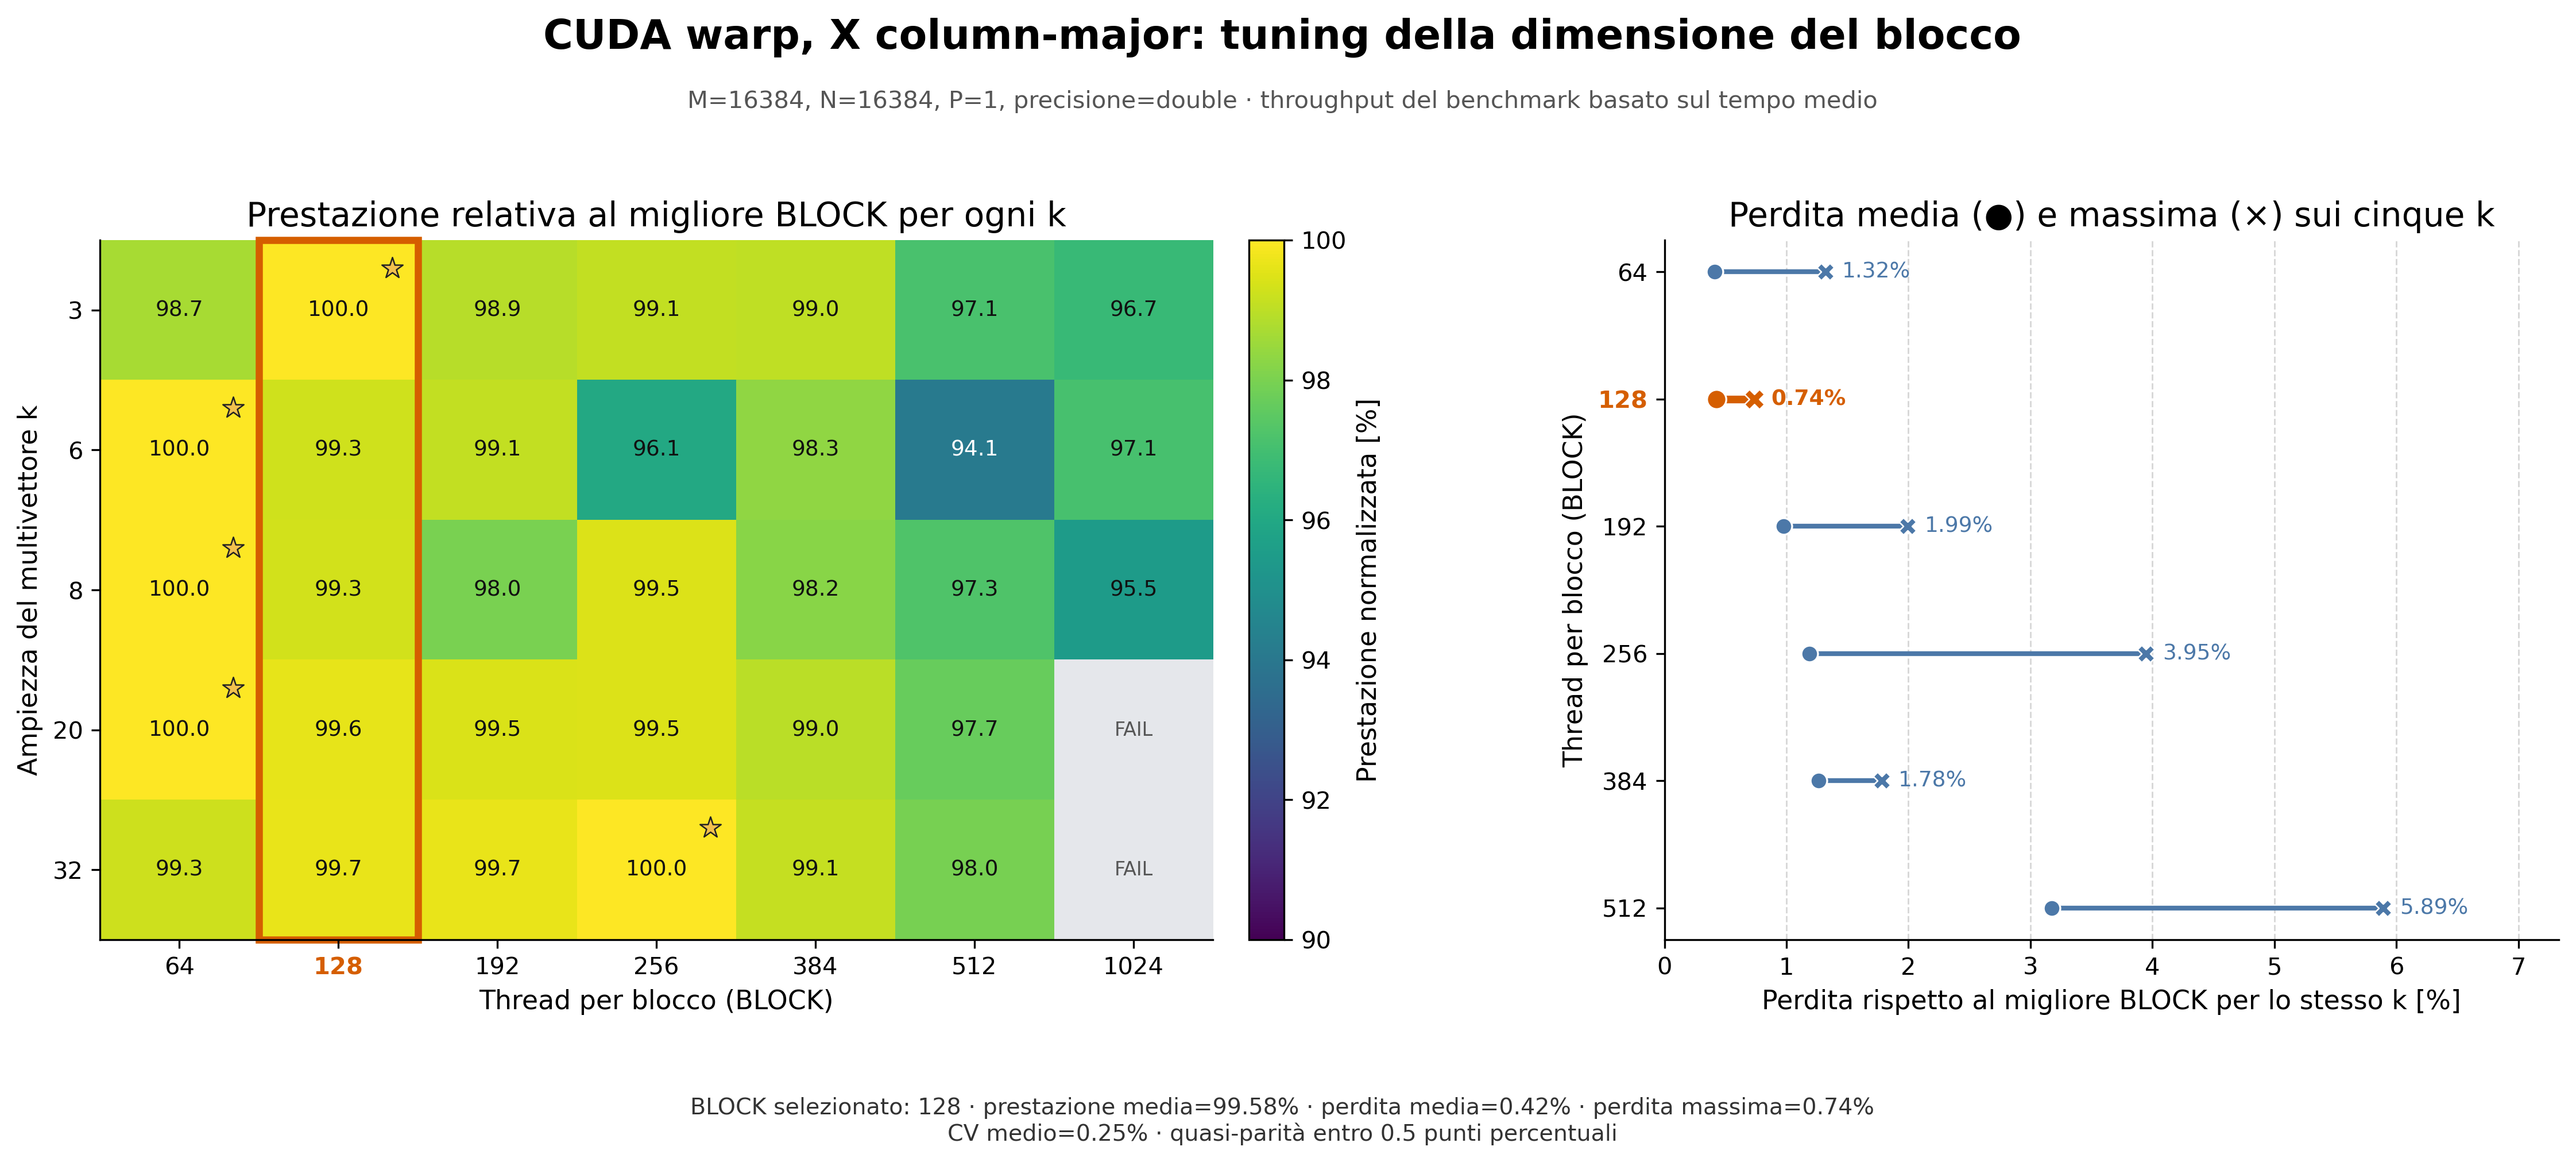
\includegraphics[width=\linewidth]{img/fase1/campagna_VAS_block_k_tuning/campagna_VAS_block_k_tuning_summary_cuda_warp_xcolumn.png}
  \caption{\kernelname{cuda\_warp}, $X$ column-major.}
\end{subfigure}

\caption{Campagna 1.1: prestazione normalizzata per $(\code{BLOCK}, k)$ a
sinistra, perdita media e massima sui cinque $k$ a destra. Le celle
\code{FAIL} sono i lanci non riusciti a \code{BLOCK}$=1024$.}
\label{fig:ris-block}
\end{figure}

\begin{figure}[H]
\centering
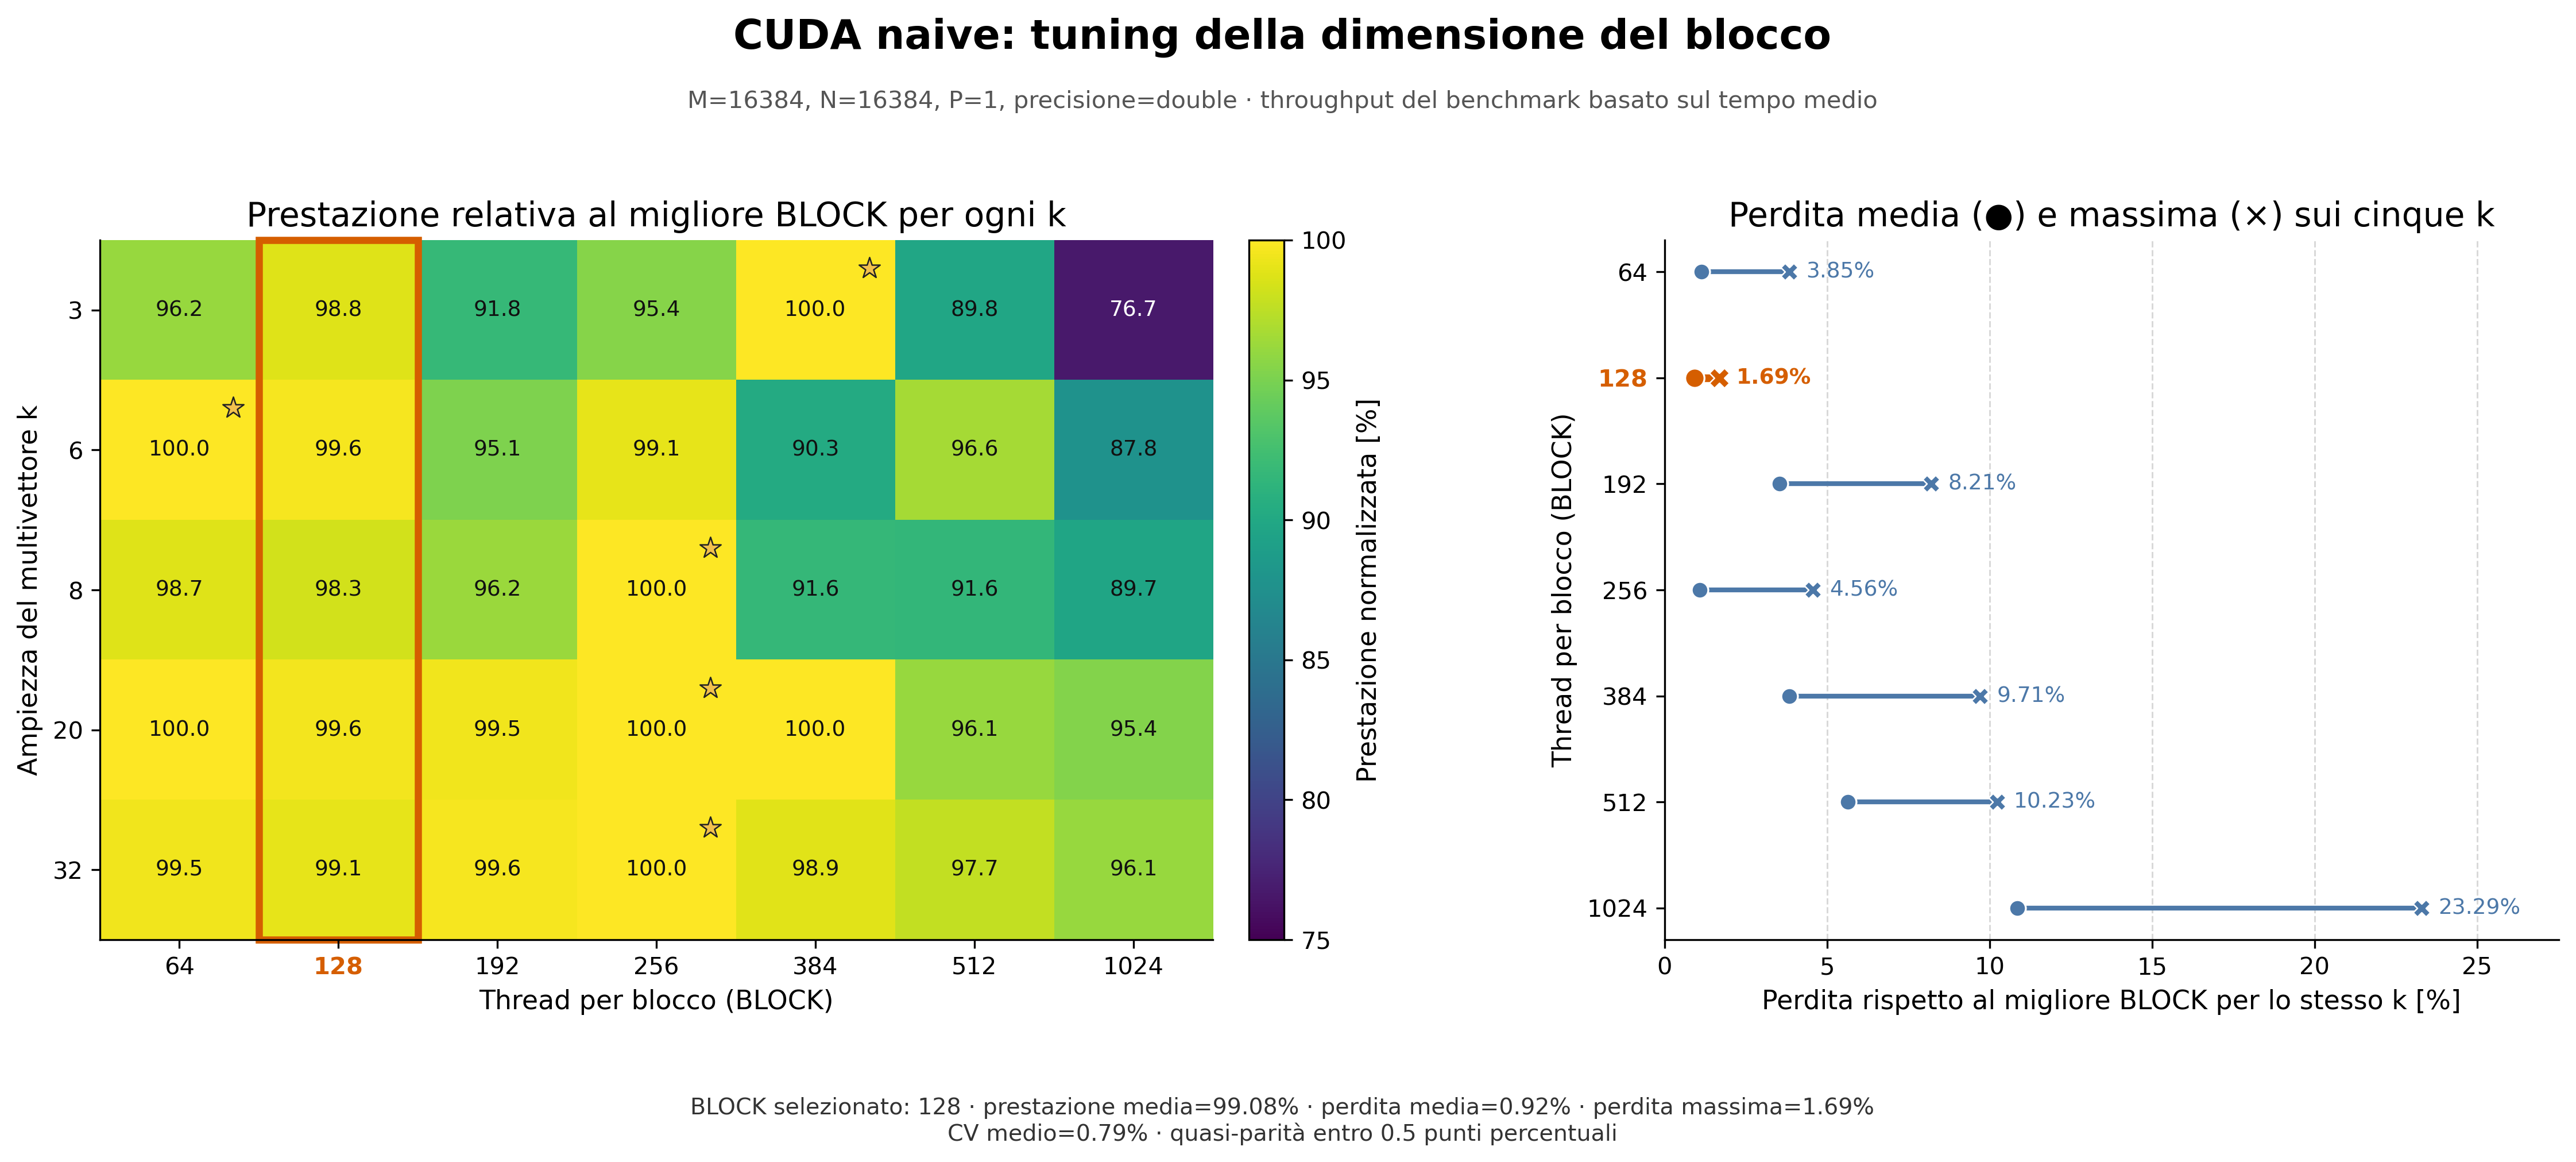
\includegraphics[width=\linewidth]{img/fase1/campagna_VAS_block_k_tuning/campagna_VAS_block_k_tuning_summary_cuda_naive.png}
\caption{Campagna 1.1: stessa lettura per \kernelname{cuda\_naive}, l'unico
kernel che completa anche a \code{BLOCK}$=1024$.}
\label{fig:ris-block-naive}
\end{figure}

\subsubsection*{Lettura}

\textbf{La sensibilità a \code{BLOCK} dipende dalla struttura del kernel.}

\kernelname{cuda\_warp} è il backend meno sensibile nell'intervallo delle
configurazioni valide. Fra 64 e 384 thread per blocco le prestazioni rimangono
vicine all'ottimo e il valore selezionato, \code{BLOCK}=128, limita la perdita
massima allo $0{,}74\%$. Il risultato è coerente con la mappatura
warp-per-row: il lavoro associato a una riga di $Y$ è già definito alla
granularità del warp, per cui modificare la dimensione del blocco cambia
principalmente quanti warp vengono raggruppati nello stesso blocco, senza
modificare il lavoro assegnato a ciascuno di essi.

\textbf{Non emerge una regola semplice basata sulla sola dimensione del
blocco.}

Per \kernelname{cuda\_naive}, ad esempio, le configurazioni
\code{BLOCK}=192 e \code{BLOCK}=384 risultano peggiori di 128 e 256, ma lo
stesso andamento non si ripete in modo uniforme sugli altri kernel.
Analogamente, \code{BLOCK}=512 produce per \kernelname{cuda\_warp} una perdita
maggiore rispetto a blocchi più piccoli. Il numero di thread per blocco non è
quindi sufficiente, da solo, a spiegare le differenze osservate. Alla
geometria del lancio si aggiungono infatti il consumo di registri per thread.

\textbf{I fallimenti a \code{BLOCK}=1024 costituiscono un ulteriore limite
della configurazione.}

Con 1024 thread per blocco,
\kernelname{cuda\_warp}  non completa
l'esecuzione per $k=20$ e $k=32$, mentre \kernelname{cuda\_naive} continua a
essere eseguibile. La differenza è coerente con la diversa pressione sui
registri: il kernel naive mantiene un solo accumulatore per thread, mentre
nelle istanze specializzate dei due kernel warp ogni lane mantiene un vettore
di $k$ accumulatori.

\textbf{Esito della campagna.}
Il criterio di robustezza porta a selezionare \code{BLOCK}=128 per
\kernelname{cuda\_naive} e per \kernelname{cuda\_warp}. In entrambi i casi la
configurazione scelta rimane molto vicina al miglior valore specifico per
ciascun $k$, evitando di ottimizzare il kernel per un solo punto della
traccia.

\subsection{Campagna 1.2 - Layout in memoria di $X$}
\label{sec:ris-layout}

\begin{table}[H]
\centering
\footnotesize
\caption{Campagna 1.2: \kernelname{cuda\_warp} con $X$ row-major e
column-major, \code{BLOCK}$=128$. L'ultima colonna è il costo della conversione
di $X$, che è preprocessing e non entra in $T$.}
\label{tab:ris-layout}
\begin{tabular}{@{}rrrrrr@{}}
\toprule
$k$ & row-major & column-major & speedup & $t_{\text{kernel}}$ row & $t_{\text{convert}}$ \\
    & [GFLOPS] & [GFLOPS] & col/row & [\si{\milli\second}] & [\si{\milli\second}] \\
\midrule
3  & 297,3 & 300,3 & 1,01 & 5,4   & 0,26 \\
6  & 352,0 & 351,4 & 1,00 & 9,2   & 0,57 \\
8  & 182,6 & 350,3 & 1,92 & 23,5  & 0,88 \\
20 & 174,1 & 351,4 & 2,02 & 61,7  & 2,43 \\
32 & 92,2  & 352,5 & 3,82 & 186,4 & 3,32 \\
\bottomrule
\end{tabular}
\end{table}

\begin{figure}[H]
\centering
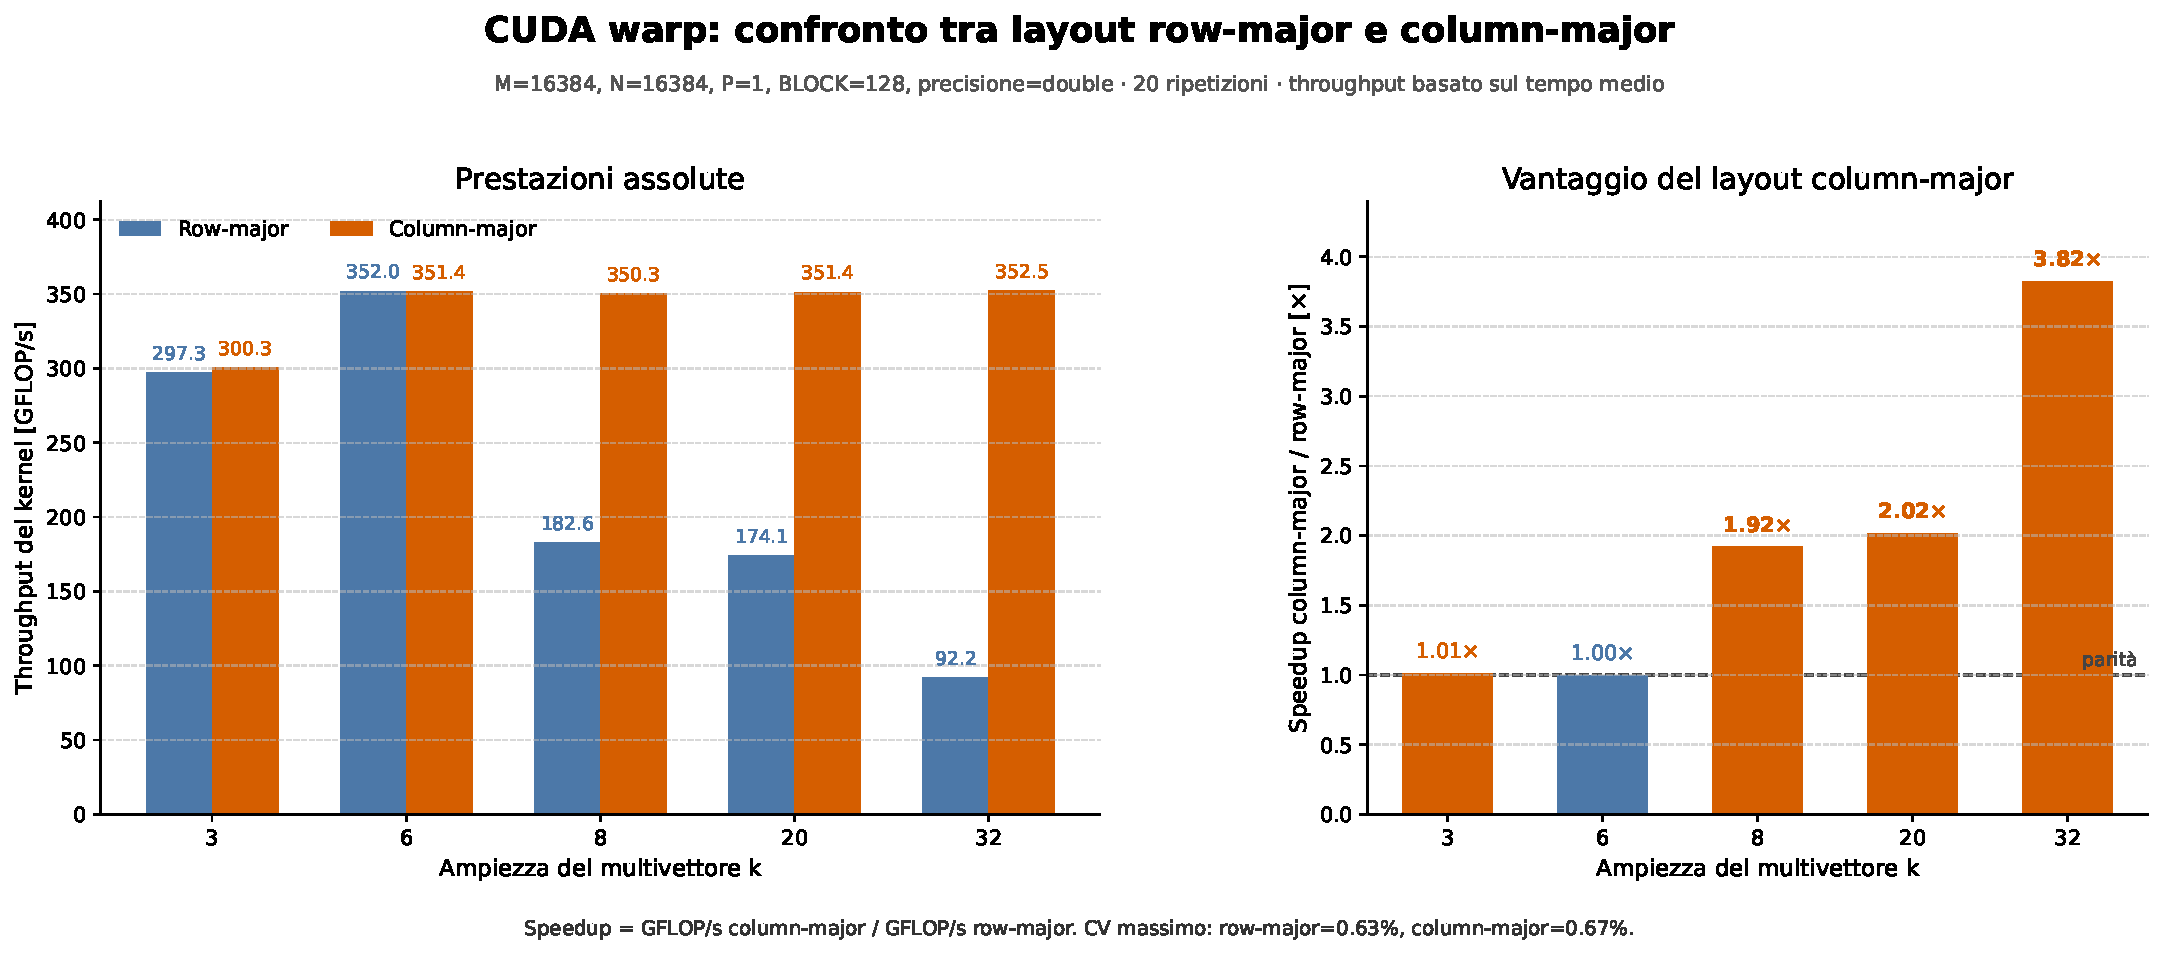
\includegraphics[width=\linewidth]{img/fase1/campagna_VAS_2_row_major/campagna_VAS_2_layout_comparison}
\caption{Campagna 1.2: prestazioni assolute (sinistra) e vantaggio del layout
column-major (destra). CV massimo: $0{,}63\%$ row-major, $0{,}67\%$
column-major.}
\label{fig:ris-layout}
\end{figure}

\subsubsection*{Lettura}

\textbf{L'effetto del layout emerge a partire da $k=8$.}

Per $k=3$ e $k=6$ le due varianti hanno prestazioni molto simili:
lo speedup del layout column-major vale rispettivamente $1{,}01\times$ e
$1{,}00\times$, con coefficienti di variazione inferiori allo $0{,}7\%$.
In questa regione l'eventuale vantaggio è quindi dello stesso ordine della
dispersione delle misure e non è sufficientemente marcato da attribuirgli un
significato prestazionale.

A partire da $k=8$ il comportamento cambia nettamente: il layout
column-major raggiunge uno speedup di $1{,}92\times$, che sale a
$2{,}02\times$ per $k=20$ e a $3{,}82\times$ per $k=32$.

Il vantaggio cresce
quindi all'aumentare della larghezza del multivettore e rende il layout
column-major la scelta naturale per \kernelname{cuda\_warp} nelle campagne
successive.

\textbf{L'andamento è coerente con il pattern di accesso previsto dal kernel.}

In \kernelname{cuda\_warp} lane consecutive elaborano valori consecutivi
dell'indice $j$. Per una colonna $c$ fissata, con $X$ row-major esse richiedono

\[
X[j_0][c],\;
X[j_0+1][c],\;
\ldots,\;
X[j_0+31][c],
\]

che nel buffer sono separati da uno stride di $k$ elementi. All'aumentare di
$k$ gli indirizzi richiesti dalle lane dello stesso warp risultano quindi
sempre più distanti, rendendo meno favorevole il raggruppamento degli accessi
alla global memory.

Con $X$ column-major gli stessi elementi sono invece \emph{consecutivi} in memoria.
Il kernel mantiene invariata la propria mappatura warp-per-row, ma le richieste
delle lane possono essere servite mediante accessi molto più compatti. La
crescita del vantaggio con $k$ è quindi coerente con l'ipotesi che il layout
row-major penalizzi progressivamente il percorso di lettura di $X$.

I risultati mostrano che la differenza fra i layout diventa rilevante proprio quando
aumenta lo stride fra gli elementi letti simultaneamente dalle lane.

\textbf{Il confronto chiarisce anche il ruolo della shared memory.}

\kernelname{cuda\_warp\_smem} mantiene $X$ nel layout row-major, ma evita che
il pattern strided del kernel \code{cuda_warp} venga ripetuto direttamente sulla global
memory. Il tile di $X$ viene prima caricato cooperativamente dai thread del
blocco, utilizzando accessi globali contigui, e viene successivamente
consumato dalla shared memory secondo la solita mappatura warp-per-row.

Le due varianti affrontano quindi lo stesso limite del percorso row-major con
strategie differenti: \kernelname{cuda\_warp} modifica la rappresentazione
fisica di $X$, mentre \kernelname{cuda\_warp\_smem} mantiene il layout
originario e modifica il percorso attraverso cui i dati raggiungono le lane.
Il confronto conclusivo della Fase~1 permette di valutare quale delle due
strategie risulti più conveniente nel regime studiato.


\subsection{Campagna 1.3 - Granularità del tile}
\label{sec:ris-granularita}

\begin{table}[H]
\centering
\footnotesize
\caption{Campagna 1.3: prestazione normalizzata di \kernelname{cuda\_warp\_smem}
per ogni coppia $(\code{BLOCK}, g)$, in percentuale dell'ottimo per lo stesso
$k$. Media sui cinque $k$ e caso peggiore. In grassetto la coppia selezionata.}
\label{tab:ris-granularita}
\begin{tabular}{@{}rrrrrrrrr@{}}
\toprule
& \multicolumn{2}{c}{$g = 1$} & \multicolumn{2}{c}{$g = 8$}
& \multicolumn{2}{c}{$g = 16$} & \multicolumn{2}{c}{$g = 32$} \\
\cmidrule(lr){2-3}\cmidrule(lr){4-5}\cmidrule(lr){6-7}\cmidrule(lr){8-9}
\code{BLOCK} & media & peggiore & media & peggiore & media & peggiore & media & peggiore \\
\midrule
64  & 83,6 & 54,7 & 82,7 & 53,8 & 77,4 & 46,2 & 86,8 & 61,0 \\
128 & 88,0 & 51,3 & 84,3 & 50,5 & 82,2 & 50,4 & 98,7 & 97,1 \\
192 & 79,0 & 67,4 & 76,5 & 66,4 & 87,7 & 71,9 & 94,9 & 81,1 \\
256 & 85,0 & 65,5 & 98,1 & 94,4 & 96,7 & 87,8 & \textbf{99,0} & \textbf{98,5} \\
384 & 89,1 & 80,0 & 89,9 & 78,6 & 89,5 & 76,0 & 90,5 & 80,2 \\
512 & 91,9 & 82,8 & 92,3 & 90,7 & 90,6 & 86,0 & 92,2 & 89,7 \\
\bottomrule
\end{tabular}
\end{table}

\begin{figure}[H]
\centering
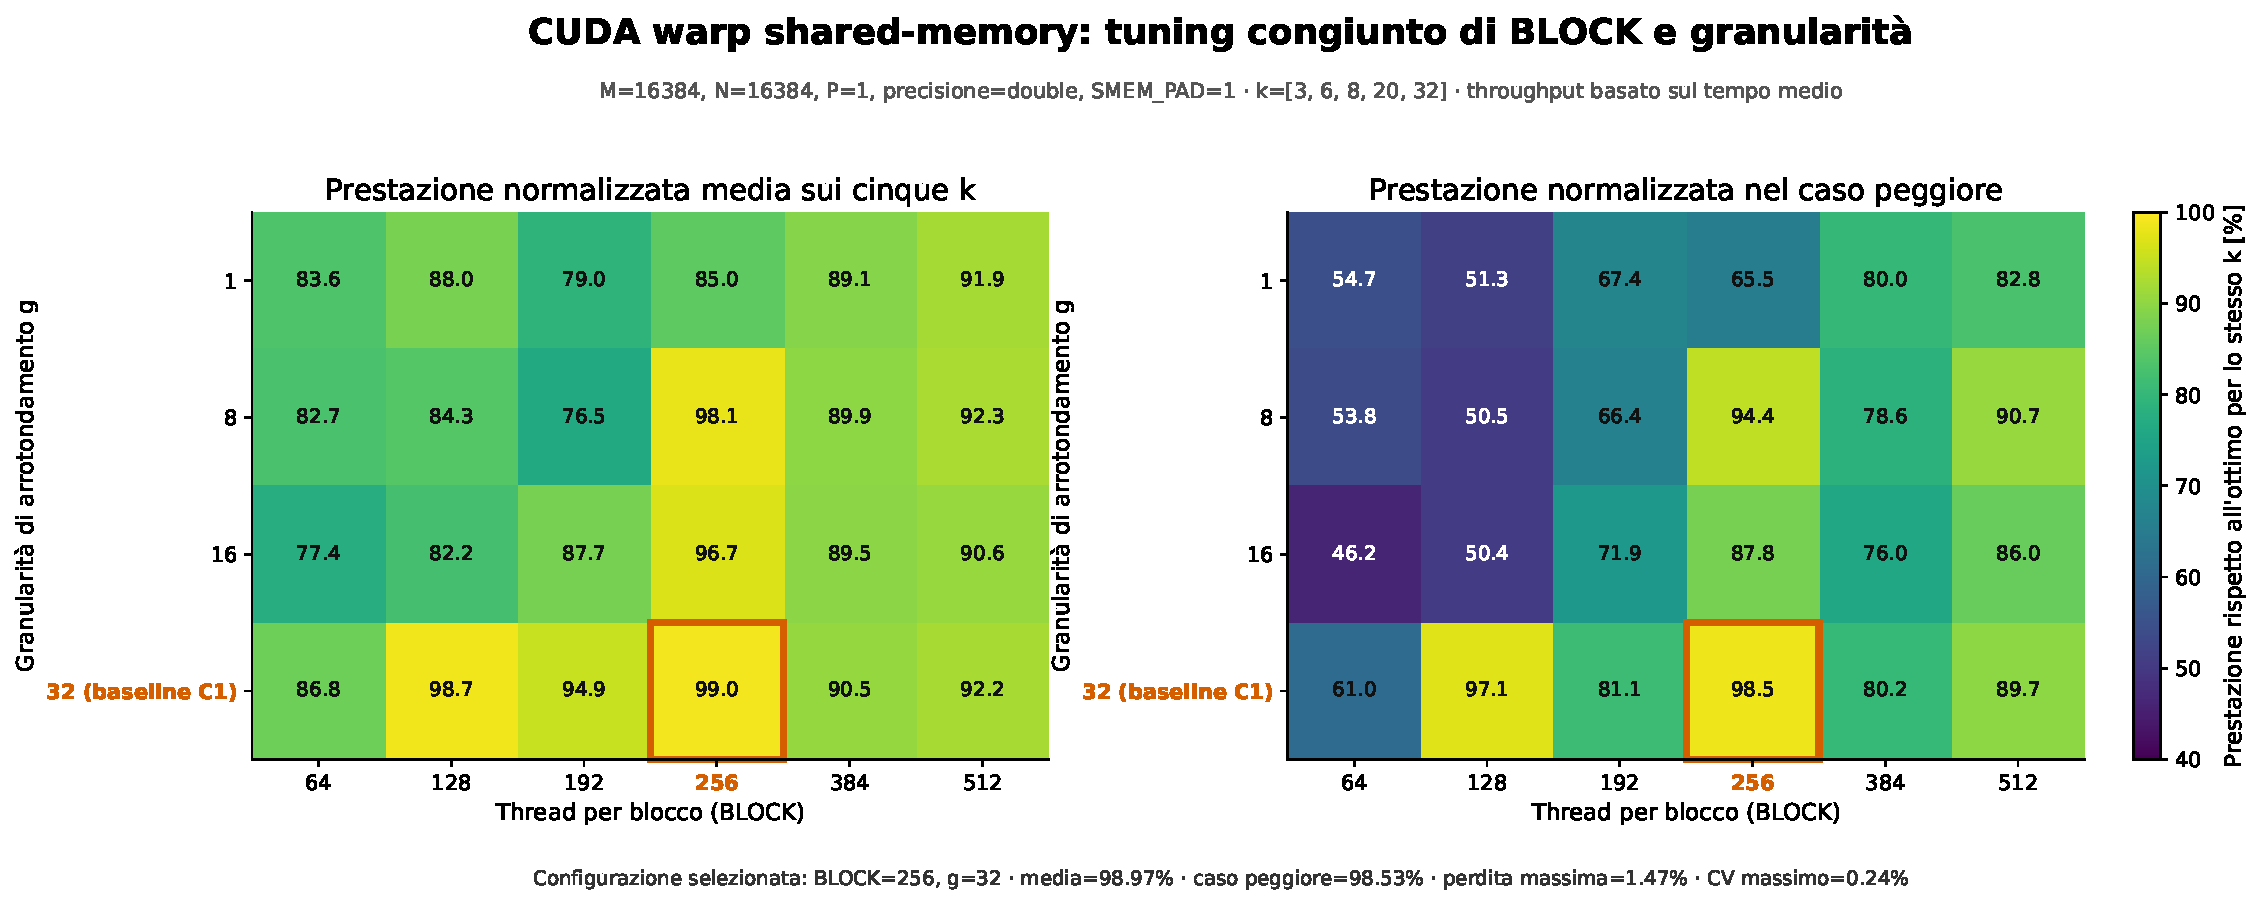
\includegraphics[width=\linewidth]{img/fase1/campagna_VAS_5_smem_granularity_tuning/campagna_VAS_5_joint_tuning_summary}
\caption{Campagna 1.4: tuning congiunto di \code{BLOCK} e granularità. A
sinistra la prestazione normalizzata media sui cinque $k$, a destra il caso
peggiore.}
\label{fig:ris-granularita}
\end{figure}

\begin{figure}[H]
\centering
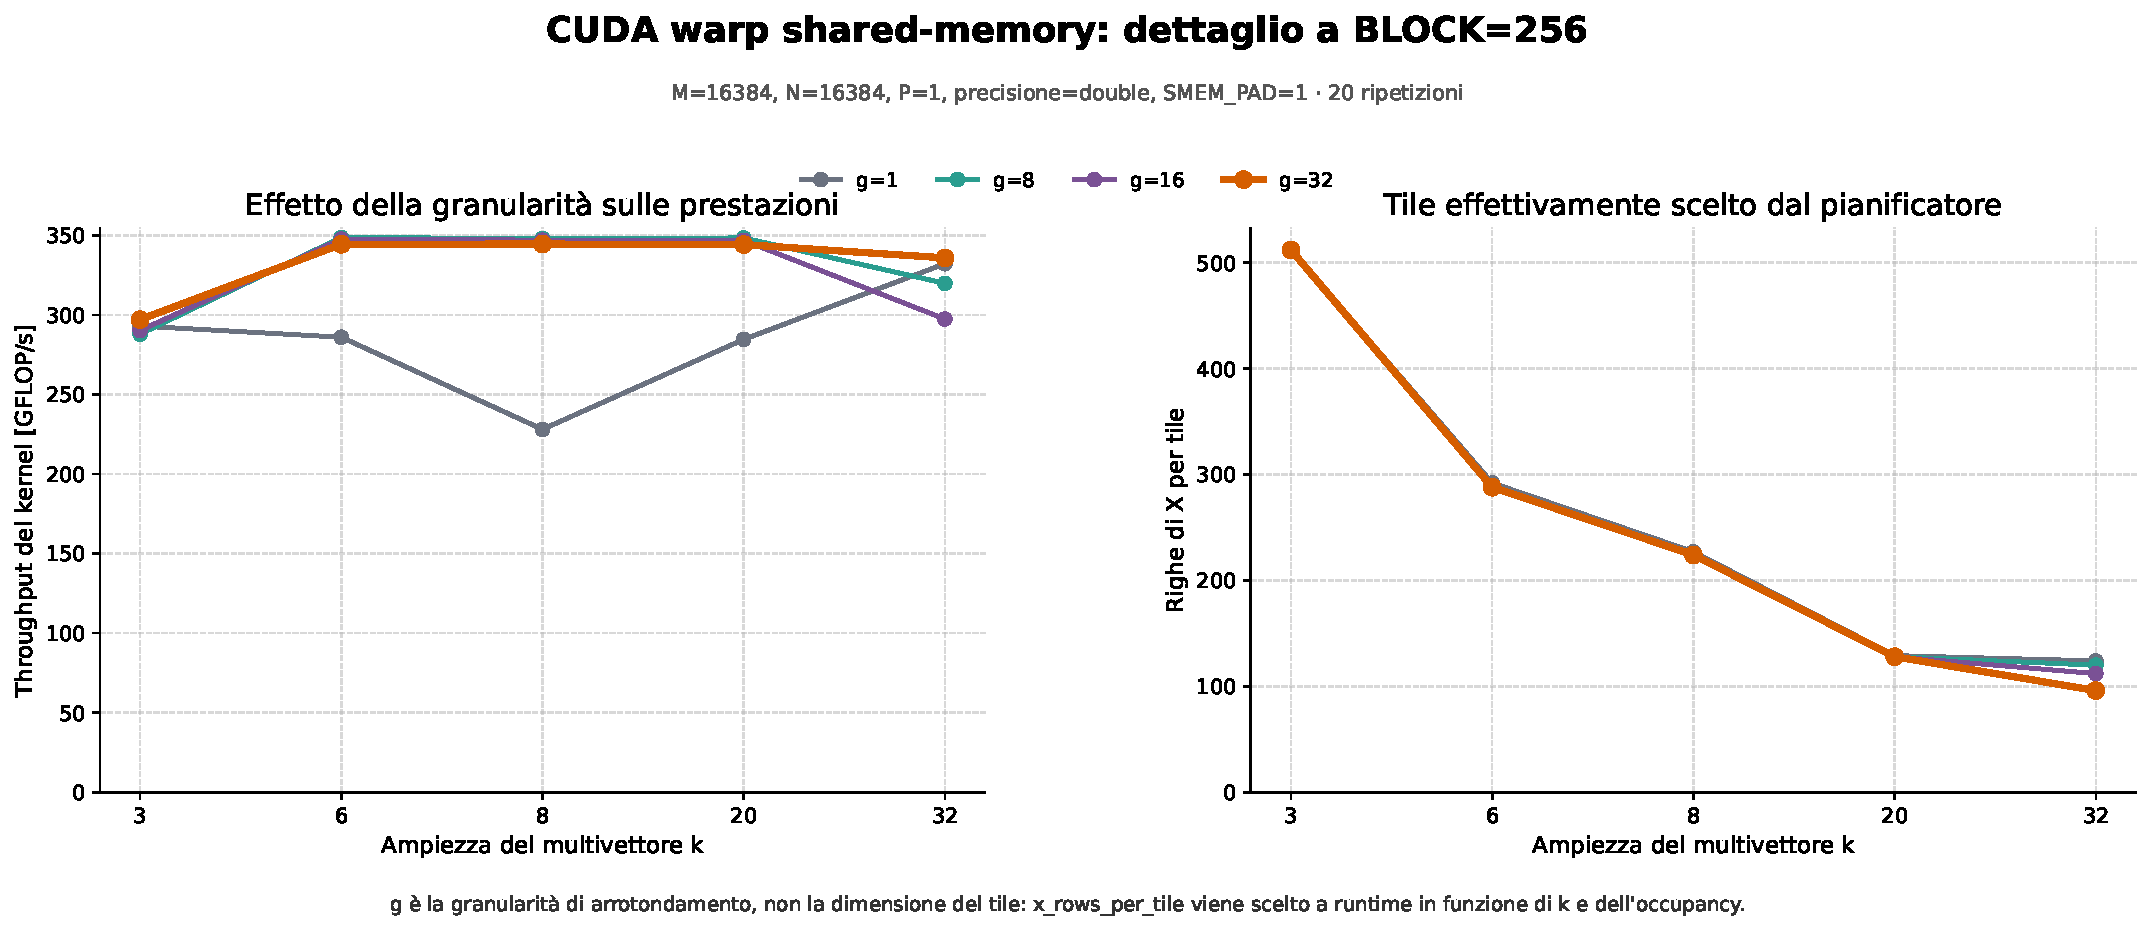
\includegraphics[width=\linewidth]{img/fase1/campagna_VAS_5_smem_granularity_tuning/campagna_VAS_5_block256_detail}
\caption{Campagna 1.4: dettaglio a \code{BLOCK}$=256$. A destra il piano di
tiling effettivamente scelto a runtime, che dipende da $k$ e non da $g$ se non
attraverso l'arrotondamento.}
\label{fig:ris-granularita-dettaglio}
\end{figure}

\subsubsection*{Lettura}

\textbf{Lo sweep congiunto conferma che \code{BLOCK} e granularità non possono
essere scelti indipendentemente.}

La configurazione preferibile cambia infatti al variare di $g$. Con
$g=1$ il valore medio più alto si ottiene a \code{BLOCK}=512, mentre per
$g=8$, $g=16$ e $g=32$ il miglior valore medio si trova a
\code{BLOCK}=256. Anche il comportamento nel caso peggiore cambia con la
coppia considerata.

La dimensione del blocco influenza il numero di warp che cooperano nello
stesso blocco e le risorse che determinano l'\emph{occupancy}, mentre la granularità
interviene successivamente sulla dimensione del tile scelta dal
pianificatore. I due parametri agiscono quindi sullo stesso kernel attraverso
meccanismi distinti, ma non indipendenti.

\textbf{Fra le granularità considerate, $g=32$ mostra il comportamento più
robusto.}

Essa fornisce la migliore prestazione media per cinque delle sei dimensioni
di blocco considerate, con l'unica eccezione di \code{BLOCK}=512, dove
$g=8$ e $g=32$ risultano sostanzialmente equivalenti. In particolare, la
coppia

\[
(\code{BLOCK},g)=(256,32)
\]

mantiene in media il $99{,}0\%$ della migliore prestazione ottenibile per
ciascun $k$ e non scende sotto il $98{,}5\%$ nel caso peggiore.

Il risultato è coerente con il ruolo di \code{TILE\_GRANULARITY} nel kernel.
Il ciclo di consumo della shared memory assegna alla lane $\ell$ le righe

\[
j=\ell,\;\ell+32,\;\ell+64,\ldots
\]

del tile. Quando il numero di righe è multiplo di 32, tutte le lane
completano lo stesso numero di passi. Una dimensione non multipla di 32 può
invece produrre un'ultima iterazione nella quale soltanto una parte delle
lane ha ancora una riga da elaborare.

Questo non implica tuttavia che una granularità pari a 32 sia
intrinsecamente ottimale. Arrotondare il tile a multipli più grandi può
lasciare inutilizzata una parte del budget di shared memory e aumentare il
numero complessivo di tile, e quindi delle sincronizzazioni. La campagna
misura proprio il bilancio fra questi due effetti.

\textbf{La granularità rifinisce un piano determinato principalmente dal
budget di shared memory.}

Come mostra \cref{fig:ris-granularita-dettaglio}, le diverse granularità non
producono piani radicalmente differenti. Il pianificatore determina prima
quante righe sono compatibili con il budget disponibile e con l'obiettivo di
occupancy, quindi arrotonda tale valore secondo $g$ e verifica nuovamente il
numero di blocchi residenti.

Per questo motivo \code{TILE\_GRANULARITY} non determina da sola la
dimensione del tile. Ne modifica piuttosto il valore finale attorno a una
dimensione già imposta dalle risorse disponibili. L'effetto prestazionale
può quindi essere ridotto quando i diversi arrotondamenti conducono a tile
simili, oppure diventare più evidente quando cambiano il numero di passi
necessari per attraversare $X$ e, di conseguenza, il numero di
sincronizzazioni eseguite dal blocco.

\subsection{Campagna 1.4 - Padding del tile in shared memory}
\label{sec:ris-pad}

\begin{table}[H]
\centering
\footnotesize
\caption{Campagna 1.4: effetto di \code{SMEM\_PAD} su
\kernelname{cuda\_warp\_smem}, \code{BLOCK}$=256$. \code{x\_rows\_per\_tile} è
il numero di righe di $X$ che il pianificatore fa entrare nel tile.}
\label{tab:ris-pad}
\begin{tabular}{@{}rrrrrr@{}}
\toprule
$k$ & \code{PAD}=0 & \code{PAD}=1 & guadagno & \code{x\_rows} & \code{x\_rows} \\
    & [GFLOPS] & [GFLOPS] & & \code{PAD}=0 & \code{PAD}=1 \\
\midrule
3  & 292,8 & 296,7 & $+1{,}3\%$  & 672 & 512 \\
6  & 315,8 & 351,8 & $+11{,}4\%$ & 320 & 288 \\
8  & 327,5 & 352,4 & $+7{,}6\%$  & 256 & 224 \\
20 & 353,9 & 352,2 & $-0{,}5\%$  & 128 & 128 \\
32 & 177,1 & 343,7 & $+94{,}1\%$ & 128 & 96 \\
\bottomrule
\end{tabular}
\end{table}

\begin{figure}[H]
\centering
\begin{tikzpicture}
\begin{axis}[
  scpa,
  width=0.82\linewidth,
  height=5.8cm,
  xlabel={$k$},
  ylabel={GFLOPS (kernel-only)},
  xmin=0,
  xmax=35,
  ymin=150,
  ymax=370,
  xtick={3,6,8,20,32},
  legend pos=south west
]
\addplot[blue!70!black,mark=*] coordinates {
  (3,292.840) (6,315.799) (8,327.543) (20,353.851) (32,177.113)
};
\addlegendentry{\code{SMEM\_PAD}=0}
\addplot[orange!80!black,mark=square*] coordinates {
  (3,296.715) (6,351.835) (8,352.396) (20,352.218) (32,343.740)
};
\addlegendentry{\code{SMEM\_PAD}=1}
\end{axis}
\end{tikzpicture}
\caption{Campagna 1.3: confronto fra tile senza padding e con una colonna di
padding. Il caso $k=32$ rende visibile la patologia che negli altri punti è
parzialmente nascosta dal resto del lavoro del kernel.}
\label{fig:ris-pad}
\end{figure}

\subsubsection*{Lettura}

\textbf{Il caso $k=32$ conferma il comportamento patologico previsto per la
mappatura sui bank.}

Senza padding, la distanza fra due righe consecutive del tile è pari a
$k=32$ elementi. In doppia precisione ciascun elemento occupa due parole da
32 bit, quindi lo spostamento fra gli indirizzi iniziali letti da lane
consecutive vale

\[
2\cdot32 = 64 \equiv 0 \pmod{32}.
\]

Gli accessi ricadono quindi periodicamente sugli stessi bank, producendo un
forte conflitto durante la lettura del tile dalla shared memory.

Con \code{SMEM\_PAD}=1 lo stride diventa invece $33$ elementi e lo
spostamento corrispondente vale

\[
2\cdot33 = 66 \equiv 2 \pmod{32},
\]

rompendo la periodicità del caso precedente. Il risultato sperimentale è
coerente con questa previsione: a $k=32$ il throughput passa da
$177{,}1$ a $343{,}7$ GFLOPS, con un incremento del $94{,}1\%$.

Il guadagno complessivo del kernel non deve però essere interpretato come
misura diretta della molteplicità del bank conflict. Il conflitto interessa
infatti soltanto la fase in cui $X$ viene letto dalla shared memory, mentre il
tempo totale comprende anche caricamento del tile, accessi ad $A$, operazioni
aritmetiche, riduzione e sincronizzazioni.

\textbf{Negli altri valori di $k$ l'effetto del padding è meno regolare.}

Il guadagno vale $11{,}4\%$ a $k=6$ e $7{,}6\%$ a $k=8$, mentre a
$k=20$ le due configurazioni differiscono soltanto dello $0{,}5\%$ a favore
della variante senza padding. A $k=3$ il vantaggio è invece limitato
all'$1{,}3\%$.

Questi risultati mostrano che la semplice regola modulare è utile per
individuare configurazioni chiaramente patologiche, come $k=32$, ma non
costituisce da sola un modello quantitativo delle prestazioni. Il tempo
complessivo dipende anche dalla dimensione effettiva del tile, dal numero di
blocchi residenti e dalla parte del kernel non coinvolta negli accessi alla
shared memory.

\textbf{Il padding migliora il caso peggiore al costo di una minore capacità
utile del tile.}

Aggiungere una colonna modifica la dimensione di ogni riga da $k$ a $k+1$
elementi. A parità di budget di shared memory possono quindi essere mantenute
meno righe di $X$ nello stesso tile. Ad esempio, il pianificatore passa da
672 a 512 righe per $k=3$ e da 128 a 96 per $k=32$.

Le righe che non entrano nel tile corrente non vengono escluse dal calcolo,
ma vengono elaborate nei tile successivi. Il costo potenziale del padding è
quindi una riduzione della quantità di $X$ trattata in ciascuna iterazione del
tiling e, in alcuni casi, un aumento del numero complessivo di tile e delle
relative sincronizzazioni.

Nonostante questo costo, il peggioramento massimo osservato con
\code{SMEM\_PAD}=1 è soltanto dello $0{,}5\%$, mentre nel caso patologico
$k=32$ il vantaggio è vicino a un fattore due. La scelta del padding è quindi
fortemente favorevole secondo il criterio di robustezza adottato nella
Fase~1.

\textbf{Esito della campagna.}

La configurazione selezionata è quindi:

\[
\code{SMEM\_PAD}=1.
\]

\textbf{Ripercussioni sul tuning congiunto.}

Combinando questo risultato con la scelta
\code{TILE_GRANULARITY}=32 della Campagna~1.3, la configurazione definitiva di
\kernelname{cuda\_warp\_smem} diventa

\[
(\code{BLOCK},\code{SMEM\_PAD},g)=(256,1,32).
\]


Nello sweep congiunto la coppia $(256,32)$ presenta una perdita massima
dell'$1{,}5\%$ rispetto alla migliore configurazione specifica per ciascun
$k$. La scelta soddisfa quindi il criterio di robustezza adottato nella
Fase~1 e definisce definitivamente il valore di
\code{BLOCK}.

\subsection{Esito della Fase 1 - Configurazioni consolidate}
\label{sec:ris-fase1-sintesi}

Le quattro campagne precedenti determinano le configurazioni utilizzate
nelle fasi successive. I valori selezionati sono raccolti in
\cref{tab:ris-fase1-sintesi}.

\begin{table}[H]
\centering
\footnotesize
\caption{Configurazione selezionata per ciascun backend CUDA.}
\label{tab:ris-fase1-sintesi}
\begin{tabular}{@{}llll@{}}
\toprule
\textbf{Backend} & \textbf{\code{BLOCK}} & \textbf{Layout di $X$} & \textbf{Altro} \\
\midrule
\kernelname{cuda\_naive}      & 128 & row    & - \\
\kernelname{cuda\_warp}       & 128 & column & - \\
\kernelname{cuda\_warp\_smem} & 256 & row    & \code{SMEM\_PAD}=1, $g=32$ \\
\kernelname{cublas}           & -   & row    & riferimento esterno \\
\bottomrule
\end{tabular}
\end{table}

Per \kernelname{cuda\_naive} e \kernelname{cuda\_warp} la dimensione del
blocco deriva dalla Campagna~1.1. Per \kernelname{cuda\_warp} la
Campagna~1.2 seleziona inoltre il layout column-major di $X$. Le
Campagne~1.3 e~1.4 completano invece la configurazione di
\kernelname{cuda\_warp\_smem}, selezionando rispettivamente il padding e la
coppia $(\code{BLOCK},\code{TILE\_GRANULARITY})$.

Da questo punto in avanti i parametri dei backend rimangono invariati.
Le fasi successive modificano quindi le caratteristiche del problema o
dell'aritmetica, senza introdurre un nuovo tuning.










\section{Fase 2 - Caratterizzazione dimensionale}
\label{sec:ris-fase2}

La Fase~1 ha fissato, per ciascun backend CUDA, una configurazione definitiva.
Tutte quelle misure sono però state prese su un unico problema,
$M=N=\num{16384}$. Resta quindi aperta una domanda: quei risultati valgono
solo per quella taglia, oppure descrivono un comportamento più generale?

La Fase~2 risponde variando le dimensioni del problema e separando due effetti
che nella pratica si presentano sempre insieme:

\begin{itemize}
  \item la \textbf{scala}, cioè quanto è grande il problema;
  \item la \textbf{forma}, cioè il rapporto fra il numero di righe $M$ e il
  numero di colonne $N$, a parità di lavoro complessivo.
\end{itemize}

Le due domande vengono affrontate una alla volta. Prima si tiene la matrice
quadrata e si fa crescere la taglia; poi si fissa la taglia e si cambia la
forma lasciando il lavoro quasi invariato.


\subsection{Disegno della campagna}
\label{sec:ris-fase2-disegno}

La campagna considera tre scale nominali

\[
S \in \{4096,\ 8192,\ \num{16384}\}
\]

e, per ciascuna scala, tre geometrie: il caso quadrato $M=N$, il caso
``largo'' $N=2M$ e il caso ``alto'' $M=3N$. I nove punti sono

\begin{center}
\footnotesize
\begin{tabular}{@{}lccc@{}}
\toprule
& $M=N$ & $N=2M$ & $M=3N$ \\
\midrule
$S=4096$  & $4096\times4096$   & $2880\times5760$   & $7104\times2368$ \\
$S=8192$  & $8192\times8192$   & $5760\times\num{11520}$  & $\num{14208}\times4736$ \\
$S=\num{16384}$ & $\num{16384}\times\num{16384}$ & $\num{11520}\times\num{23040}$ & $\num{28416}\times9472$ \\
\bottomrule
\end{tabular}
\end{center}

Le dimensioni rettangolari non sono scelte a caso: sono state costruite in modo
che il prodotto $MN$ resti quasi uguale a quello del caso quadrato della stessa
scala. Rispetto a $S^2$, la forma $N=2M$ ha l'$1{,}12\%$ di elementi in meno e
la forma $M=3N$ lo $0{,}27\%$ in più.

Questo dettaglio è ciò che rende interpretabile il confronto. Poiché il numero
di operazioni è
$2MNk$,
tenere $MN$ costante significa tenere costante il lavoro. Se due forme della
stessa scala danno throughput diversi, la differenza non può essere attribuita
al fatto che una delle due ``fa più conti'': è una reazione del kernel alla
geometria.

Tutte le misure sono in doppia precisione, con $P=1$, $5$ warm-up e $20$
repetition misurate, e usano per ogni backend i parametri selezionati nella
Fase~1 (\cref{sec:ris-fase1-sintesi}). La grandezza riportata è sempre
\code{gflops\_kernel}, cioè il throughput del solo kernel, al netto dei
trasferimenti H2D e D2H. Il prodotto completo dei fattori dà
$3$ scale $\times$ $3$ forme $\times$ $4$ backend $\times$ $5$ valori di $k$,
cioè $180$ configurazioni misurate.


\subsection{Effetto della scala}
\label{sec:ris-fase2-scala}

Per isolare la scala si guardano soltanto le configurazioni quadrate,
$M=N=S$,
facendo crescere $S$ di un fattore $2$ per volta, cioè facendo crescere il
lavoro di un fattore $4$ per volta.

\begin{table}[H]
\centering
\footnotesize
\caption{Fase~2: \code{gflops\_kernel} dei quattro backend sul caso quadrato
$M=N=S$, per tutti i valori di $k$ misurati.}
\label{tab:ris-fase2-scala-completa}
\begin{tabular}{@{}llrrrrr@{}}
\toprule
\textbf{Scala} & \textbf{Backend}
& $k=3$ & $k=6$ & $k=8$ & $k=20$ & $k=32$ \\
\midrule

\multirow{4}{*}{$S=4096$}
& \kernelname{cuda\_naive} & 162,3 & 252,0 & 253,2 & 277,2 & 287,7 \\
& \kernelname{cuda\_warp} & 269,6 & 275,7 & 277,4 & 279,8 & 281,5 \\
& \kernelname{cuda\_warp\_smem} & 253,5 & 265,8 & 267,5 & 273,5 & 274,5 \\
& \kernelname{cublas} & 16,5 & 34,6 & 46,1 & 115,2 & 184,3 \\

\midrule

\multirow{4}{*}{$S=8192$}
& \kernelname{cuda\_naive} & 187,3 & 309,7 & 342,5 & 348,7 & 354,5 \\
& \kernelname{cuda\_warp} & 297,5 & 348,4 & 347,8 & 347,5 & 354,1 \\
& \kernelname{cuda\_warp\_smem} & 291,5 & 338,3 & 337,6 & 338,6 & 330,7 \\
& \kernelname{cublas} & 15,4 & 30,8 & 41,1 & 102,7 & 164,0 \\

\midrule

\multirow{4}{*}{$S=\num{16384}$}
& \kernelname{cuda\_naive} & 151,5 & 307,1 & 342,0 & 345,5 & 349,7 \\
& \kernelname{cuda\_warp} & 302,0 & 354,3 & 353,2 & 354,6 & 354,9 \\
& \kernelname{cuda\_warp\_smem} & 296,8 & 349,8 & 349,6 & 349,5 & 341,0 \\
& \kernelname{cublas} & 15,3 & 30,7 & 40,8 & 102,0 & 163,2 \\

\bottomrule
\end{tabular}
\end{table}

Una prima lettura della \cref{tab:ris-fase2-scala-completa} mostra due
comportamenti opposti. I tre kernel scritti nel progetto migliorano al
crescere della taglia; \kernelname{cublas} peggiora. Inoltre, per i kernel
custom quasi tutto il guadagno si concentra nel primo raddoppio, da $S=4096$ a
$S=8192$: il passaggio successivo aggiunge poco.

\subsubsection{\kernelname{cuda\_warp}}

Il caso più netto è \kernelname{cuda\_warp}. Alla scala più piccola il
throughput è praticamente insensibile a $k$: resta fra $269{,}6$ e
$281{,}5$ GFLOPS su tutto l'intervallo, cioè si muove di poco più di
$10$ GFLOPS mentre il lavoro cresce di dieci volte.

Alle due scale maggiori il comportamento cambia forma. Il valore a $k=3$ resta
isolato in basso ($297{,}5$ e $302{,}0$ GFLOPS), mentre da $k=6$ in poi il
kernel si appiattisce su un plateau: $347{,}5$–$354{,}1$ GFLOPS a $S=8192$ e
$353{,}2$–$354{,}9$ GFLOPS a $S=\num{16384}$.

Il confronto fra la prima e l'ultima scala si riassume in due numeri:

\begin{itemize}
  \item per $k\ge6$ il guadagno sta fra $1{,}26$ e $1{,}29\times$;
  \item a $k=3$ è solo di circa $1{,}12\times$.
\end{itemize}

Il punto importante non è però l'entità del guadagno, ma il fatto che a
$S=4096$ il plateau \emph{non viene mai raggiunto}, per nessun valore di $k$.
A $S=4096$ e $k=32$ il kernel fa $281{,}5$ GFLOPS, contro i $354{,}9$ dello
stesso kernel e dello stesso $k$ a $S=\num{16384}$: la differenza non dipende
dalla larghezza del multivettore, ma dalla taglia del problema.

Una taglia più piccola significa meno lavoro per singola invocazione e quindi
meno righe di $Y$ da produrre, cioè meno warp indipendenti disponibili. Le sole
misure temporali non permettono però di attribuire il deficit a un meccanismo
preciso (occupancy, latenza, comportamento delle cache o numero di blocchi
residenti). L'affermazione che i dati sostengono direttamente è più semplice e
più utile: \kernelname{cuda\_warp} raggiunge il proprio regime di plateau
soltanto quando il problema è abbastanza grande, e $S=4096$ è al di sotto di
quella soglia.

\begin{figure}[H]
\centering
\begin{tikzpicture}
\begin{axis}[
  scpa,
  xlabel={$k$},
  ylabel={GFLOPS (kernel-only)},
  xmin=0,
  xmax=35,
  ymin=240,
  ymax=410,
  xtick={3,6,8,20,32},
  legend pos=north west,
  width=0.8\linewidth,
  height=6cm
]

\addplot[black, dashed, thick, forget plot, samples=2, domain=0:35]{350};

\addplot[blue!70!black, mark=*] coordinates {
  (3,302.0) (6,354.3) (8,353.2) (20,354.6) (32,354.9)
};
\addlegendentry{$S=16384$}

\addplot[teal!70!black, mark=triangle*] coordinates {
  (3,297.5) (6,348.4) (8,347.8) (20,347.5) (32,354.1)
};
\addlegendentry{$S=8192$}

\addplot[orange!80!black, mark=square*] coordinates {
  (3,269.6) (6,275.7) (8,277.4) (20,279.8) (32,281.5)
};
\addlegendentry{$S=4096$}

\end{axis}
\end{tikzpicture}

\caption{Fase~2: \kernelname{cuda\_warp} sul caso quadrato alle tre scale,
dai valori della \cref{tab:ris-fase2-scala-completa}. La linea tratteggiata
indica il tetto FP64 nominale di \SI{350}{\giga\flop\per\second} utilizzato
nel modello.}
\label{fig:ris-fase2-scala}
\end{figure}

La figura rende visibile la differenza qualitativa: a $S=4096$ la curva è
piatta e lontana dal tetto, alle due scale maggiori sale subito e poi si
appoggia sul tetto.

\subsubsection{\kernelname{cuda\_warp\_smem}}

La variante con shared memory segue lo stesso andamento generale, ma in modo
più graduale e senza mai superare \kernelname{cuda\_warp} sul caso quadrato.

A differenza degli altri due kernel custom, qui la crescita con la scala è
monotona per ogni $k$: a $k=3$ i tre valori sono $253{,}5$, $291{,}5$ e
$296{,}8$ GFLOPS; a $k=32$ sono $274{,}5$, $330{,}7$ e $341{,}0$ GFLOPS. Il
throughput continua quindi ad aumentare anche nel passaggio da $S=8192$ a
$S=\num{16384}$, dove \kernelname{cuda\_warp} si era già fermato.

Lo scarto rispetto a \kernelname{cuda\_warp} resta comunque sempre a favore di
quest'ultimo. Alle due scale maggiori è piccolo, entro il $3\%$ per $k\le20$;
a $S=4096$ è un po' più ampio e vale il $6{,}3\%$ a $k=3$ ($269{,}6$ contro
$253{,}5$). Fa eccezione $k=32$, dove il divario si allarga anche sui problemi
grandi ($330{,}7$ contro $354{,}1$ a $S=8192$ e $341{,}0$ contro $354{,}9$ a
$S=\num{16384}$).

Si nota anche, alle due scale maggiori, un piccolo calo passando da $k=20$ a
$k=32$ ($338{,}6 \rightarrow 330{,}7$ e $349{,}5 \rightarrow 341{,}0$), che
sulle altre due varianti non compare. È l'unico punto della campagna in cui
lo staging esplicito di $X$ in shared memory sembra costare più di quanto
rende in FP64.

\subsubsection{\kernelname{cuda\_naive}}

Il kernel di riferimento interno ha un andamento meno regolare, e il motivo è
concentrato tutto a $k=3$.

Per $k\ge8$ \kernelname{cuda\_naive} cresce con la scala e arriva dove
arrivano gli altri: $342{,}0$–$349{,}7$ GFLOPS a $S=\num{16384}$, cioè
sostanzialmente il valore di \kernelname{cuda\_warp}. A $k=3$, invece, la
successione è

\[
162{,}3 \rightarrow 187{,}3 \rightarrow 151{,}5 \quad\text{GFLOPS},
\]

cioè non monotona: il valore migliore si osserva alla scala intermedia e quello
peggiore alla scala massima.

Il confronto fra i due kernel a $k=3$ è quindi il risultato più stabile della
tabella, e non si attenua crescendo: \kernelname{cuda\_warp} vale
$1{,}66\times$ a $S=4096$ e arriva a $1{,}99\times$ a $S=\num{16384}$. Il
vantaggio della mappatura a warp non è un throughput di picco più alto, ma il
fatto di raggiungerlo già con multivettori stretti.

\subsubsection{\kernelname{cublas}}

Il riferimento esterno si comporta in modo qualitativamente diverso da tutti i
kernel custom, e la tabella lo mostra senza bisogno di altre misure.

Si prenda la riga $S=\num{16384}$ e si parta da $k=3$, dove il valore è
$15{,}3$ GFLOPS. Moltiplicando per $k/3$ si ottiene $30{,}6$, $40{,}8$,
$102{,}0$ e $163{,}2$, contro i $30{,}7$, $40{,}8$, $102{,}0$ e $163{,}2$
effettivamente misurati. Il throughput è quindi \emph{proporzionale} a $k$, e
poiché

\[
\text{GFLOPS} = \frac{2MNk}{t_{\text{kernel}}},
\]

questo equivale a dire che $t_{\text{kernel}}$ non dipende da $k$. La stessa
verifica riesce a $S=8192$ e, da $k=6$ in poi, anche a $S=4096$.

Il costo della chiamata è dunque determinato dallo streaming di $A$, non dal
lavoro effettivamente richiesto: con $k\le32$ una GEMM general-purpose paga
quasi lo stesso tempo che pagherebbe per un multivettore molto più largo.

Sulla scala, cuBLAS perde invece throughput: a ogni $k$ il valore a $S=8192$
è circa l'$89\%$ di quello a $S=4096$, e a $S=\num{16384}$ resta lì. Il
divario rispetto a \kernelname{cuda\_warp} sul problema più grande va da
$19{,}7\times$ a $k=3$ a $2{,}2\times$ a $k=32$: si riduce al crescere di $k$,
come previsto, ma non si annulla nell'intervallo richiesto dalla traccia.


\subsection{Effetto della forma}
\label{sec:ris-fase2-forma}

La seconda domanda riguarda la geometria. Per ogni scala si confrontano le tre
forme $M=N$, $N=2M$ e $M=3N$, che come detto hanno lo stesso $MN$ entro
l'$1{,}2\%$.

Il confronto va letto così: a parità di scala e di $k$, il numero di
operazioni è lo stesso in tutte e tre le righe di una tabella, quindi ogni
differenza verticale è sensibilità alla forma. Un modo compatto per
riassumere ciascun blocco è lo \emph{scarto} fra la forma migliore e la
peggiore, espresso in percentuale della peggiore.

\subsubsection{\kernelname{cuda\_warp}}

\begin{table}[H]
\centering
\footnotesize
\caption{Fase~2: \code{gflops\_kernel} di \kernelname{cuda\_warp} sulle tre
forme e sulle tre scale.}
\label{tab:ris-fase2-warp}
\begin{tabular}{@{}llrrrrr@{}}
\toprule
\textbf{Scala} & \textbf{Forma}
& $k=3$ & $k=6$ & $k=8$ & $k=20$ & $k=32$ \\
\midrule

\multirow{3}{*}{$S=4096$}
& $M=N$  & 269,6 & 275,7 & 277,4 & 279,8 & 281,5 \\
& $N=2M$ & 280,8 & 308,9 & 310,4 & 289,0 & 292,0 \\
& $M=3N$ & 285,7 & 330,0 & 330,5 & 278,0 & 281,4 \\

\midrule

\multirow{3}{*}{$S=8192$}
& $M=N$  & 297,5 & 348,4 & 347,8 & 347,5 & 354,1 \\
& $N=2M$ & 296,6 & 353,5 & 351,5 & 354,7 & 357,5 \\
& $M=3N$ & 297,8 & 343,1 & 342,7 & 345,9 & 347,6 \\

\midrule

\multirow{3}{*}{$S=\num{16384}$}
& $M=N$  & 302,0 & 354,3 & 353,2 & 354,6 & 354,9 \\
& $N=2M$ & 300,0 & 356,0 & 355,8 & 357,4 & 356,7 \\
& $M=3N$ & 301,7 & 349,6 & 349,8 & 351,9 & 352,4 \\

\bottomrule
\end{tabular}
\end{table}

Alla scala più piccola la forma conta molto. A $S=4096$ e $k=6$ il throughput
passa da $275{,}7$ GFLOPS nel caso quadrato a $308{,}9$ per $N=2M$ e
$330{,}0$ per $M=3N$; a $k=8$ l'andamento è quasi identico
($277{,}4 \rightarrow 310{,}4 \rightarrow 330{,}5$). In entrambi i casi lo
scarto fra la forma migliore e la peggiore è vicino al $20\%$.

Non esiste però una forma sempre vincente, nemmeno a scala fissa. Sulla stessa
riga di scala, a $k=20$ la migliore è $N=2M$ ($289{,}0$ contro $279{,}8$ e
$278{,}0$) e a $k=32$ vale lo stesso ($292{,}0$ contro $281{,}5$ e $281{,}4$).
La forma $M=3N$, che era la migliore ai $k$ stretti, diventa la peggiore ai
$k$ larghi. L'effetto della geometria dipende quindi anche da $k$.

Crescendo di scala la dispersione crolla. A $S=8192$ lo scarto massimo su
tutti i $k$ è del $3{,}1\%$, a $S=\num{16384}$ dell'$1{,}8\%$: a $k=6$, per
esempio, i tre valori sono $354{,}3$, $356{,}0$ e $349{,}6$ GFLOPS.

Questo comportamento si lega alla struttura del kernel. \kernelname{cuda\_warp}
assegna un warp a ogni riga di $Y$, quindi cambiare il rapporto $M{:}N$ a
prodotto costante modifica due cose insieme: quante righe indipendenti
esistono, e quanto è lunga la riduzione lungo $N$ che ciascun warp deve
percorrere. Nel caso $M=3N$ ci sono più righe ma riduzioni più corte; nel caso
$N=2M$ avviene il contrario.

La campagna non permette di separare quantitativamente i due effetti, e il
vantaggio di $M=3N$ a $S=4096$ non va quindi letto come prova che ``più righe
è meglio''. Il risultato solido è un altro: quando il problema è abbastanza
grande da fornire comunque parallelismo in abbondanza, la forma smette
praticamente di contare.

\subsubsection{\kernelname{cuda\_naive}}

\begin{table}[H]
\centering
\footnotesize
\caption{Fase~2: \code{gflops\_kernel} di \kernelname{cuda\_naive} sulle tre
forme e sulle tre scale.}
\label{tab:ris-fase2-naive}
\begin{tabular}{@{}llrrrrr@{}}
\toprule
\textbf{Scala} & \textbf{Forma}
& $k=3$ & $k=6$ & $k=8$ & $k=20$ & $k=32$ \\
\midrule

\multirow{3}{*}{$S=4096$}
& $M=N$  & 162,3 & 252,0 & 253,2 & 277,2 & 287,7 \\
& $N=2M$ & 149,9 & 274,2 & 329,1 & 275,5 & 300,7 \\
& $M=3N$ & 165,9 & 297,7 & 324,5 & 283,5 & 295,8 \\

\midrule

\multirow{3}{*}{$S=8192$}
& $M=N$  & 187,3 & 309,7 & 342,5 & 348,7 & 354,5 \\
& $N=2M$ & 160,3 & 284,8 & 326,0 & 345,6 & 356,5 \\
& $M=3N$ & 140,1 & 296,0 & 341,4 & 346,8 & 354,4 \\

\midrule

\multirow{3}{*}{$S=\num{16384}$}
& $M=N$  & 151,5 & 307,1 & 342,0 & 345,5 & 349,7 \\
& $N=2M$ & 134,0 & 277,4 & 349,9 & 342,0 & 347,6 \\
& $M=3N$ & 132,6 & 289,2 & 348,2 & 342,9 & 346,1 \\

\bottomrule
\end{tabular}
\end{table}

\kernelname{cuda\_naive} è il backend più sensibile alla forma, e soprattutto
è l'unico in cui la sensibilità \emph{non} sparisce crescendo di scala: cambia
solo il valore di $k$ in cui si manifesta.

A $S=4096$ il massimo scarto è del $30{,}0\%$ ed è a $k=8$ ($253{,}2$ nel caso
quadrato contro $329{,}1$ per $N=2M$): le forme rettangolari sono molto
migliori.

A $S=8192$ e $S=\num{16384}$ il segno si rovescia e il fenomeno si sposta a
$k=3$. Alla scala intermedia lo scarto è del $33{,}7\%$, il più grande
dell'intera campagna ($187{,}3$ per il quadrato contro $140{,}1$ per $M=3N$);
alla scala massima è ancora del $14{,}2\%$ ($151{,}5$ contro $132{,}6$).
Adesso è il caso quadrato a essere nettamente il migliore.

Per $k\ge20$, invece, le tre forme si avvicinano molto: lo scarto è del
$4{,}5\%$ a $S=4096$ e scende sotto l'$1\%$ alle due scale maggiori.

La lettura complessiva è coerente con quanto visto sulla scala: il punto
debole di \kernelname{cuda\_naive} sono i multivettori stretti, e proprio lì il
kernel resta esposto alla geometria del problema anche quando il problema è
grande.

\subsubsection{\kernelname{cuda\_warp\_smem}}

\begin{table}[H]
\centering
\footnotesize
\caption{Fase~2: \code{gflops\_kernel} di \kernelname{cuda\_warp\_smem} sulle
tre forme e sulle tre scale.}
\label{tab:ris-fase2-smem}
\begin{tabular}{@{}llrrrrr@{}}
\toprule
\textbf{Scala} & \textbf{Forma}
& $k=3$ & $k=6$ & $k=8$ & $k=20$ & $k=32$ \\
\midrule

\multirow{3}{*}{$S=4096$}
& $M=N$  & 253,5 & 265,8 & 267,5 & 273,5 & 274,5 \\
& $N=2M$ & 272,5 & 316,9 & 318,6 & 268,5 & 262,0 \\
& $M=3N$ & 282,3 & 312,3 & 319,2 & 268,5 & 263,0 \\

\midrule

\multirow{3}{*}{$S=8192$}
& $M=N$  & 291,5 & 338,3 & 337,6 & 338,6 & 330,7 \\
& $N=2M$ & 291,4 & 347,9 & 348,3 & 349,6 & 342,4 \\
& $M=3N$ & 293,6 & 338,0 & 338,7 & 341,5 & 333,8 \\

\midrule

\multirow{3}{*}{$S=\num{16384}$}
& $M=N$  & 296,8 & 349,8 & 349,6 & 349,5 & 341,0 \\
& $N=2M$ & 289,7 & 349,7 & 349,6 & 350,3 & 341,6 \\
& $M=3N$ & 295,8 & 346,9 & 345,8 & 347,3 & 338,8 \\

\bottomrule
\end{tabular}
\end{table}

La variante con shared memory riproduce la convergenza già vista per
\kernelname{cuda\_warp}: scarto massimo del $19{,}3\%$ a $S=4096$, del
$3{,}5\%$ a $S=8192$ e del $2{,}4\%$ a $S=\num{16384}$.

Alla scala piccola, però, l'effetto cambia segno con $k$ in modo molto
marcato. A $k=6$ e $k=8$ le forme rettangolari vincono nettamente
($267{,}5 \rightarrow 318{,}6$ e $319{,}2$ a $k=8$), mentre a $k=20$ e $k=32$
perdono e il caso quadrato diventa il migliore ($274{,}5$ contro $262{,}0$ e
$263{,}0$ a $k=32$).

Alla scala intermedia emerge invece una regolarità pulita: per $k\ge6$ la
forma $N=2M$ è la migliore a tutti i valori di $k$, con un vantaggio di circa
il $3\%$ (a $k=3$ le tre forme sono già indistinguibili, entro lo $0{,}7\%$). Alla scala massima anche questo vantaggio si assottiglia e le tre
forme diventano intercambiabili.

Va sottolineato un punto che riguarda l'interpretazione. La configurazione del
backend resta identica lungo tutta la campagna: a parità di $k$, il numero di
blocchi residenti per SM e il numero di righe di $X$ caricate per tile non
cambiano al variare del rapporto $M{:}N$. Le differenze osservate fra le forme
non sono quindi riconducibili a una diversa scelta del piano di tiling.

\subsubsection{\kernelname{cublas}}

\begin{table}[H]
\centering
\footnotesize
\caption{Fase~2: \code{gflops\_kernel} di \kernelname{cublas} sulle tre
forme e sulle tre scale.}
\label{tab:ris-fase2-cublas}
\begin{tabular}{@{}llrrrrr@{}}
\toprule
\textbf{Scala} & \textbf{Forma}
& $k=3$ & $k=6$ & $k=8$ & $k=20$ & $k=32$ \\
\midrule

\multirow{3}{*}{$S=4096$}
& $M=N$  & 16,5 & 34,6 & 46,1 & 115,2 & 184,3 \\
& $N=2M$ & 13,6 & 32,5 & 43,4 & 108,2 & 173,4 \\
& $M=3N$ & 16,0 & 32,0 & 42,7 & 106,6 & 170,8 \\

\midrule

\multirow{3}{*}{$S=8192$}
& $M=N$  & 15,4 & 30,8 & 41,1 & 102,7 & 164,0 \\
& $N=2M$ & 16,3 & 32,5 & 43,4 & 108,2 & 173,5 \\
& $M=3N$ & 15,9 & 31,9 & 42,5 & 106,1 & 169,6 \\

\midrule

\multirow{3}{*}{$S=\num{16384}$}
& $M=N$  & 15,3 & 30,7 & 40,8 & 102,0 & 163,2 \\
& $N=2M$ & 16,0 & 32,1 & 42,8 & 106,9 & 170,9 \\
& $M=3N$ & 15,8 & 31,6 & 42,1 & 105,3 & 168,5 \\

\bottomrule
\end{tabular}
\end{table}

cuBLAS è l'unico backend in cui la sensibilità alla forma \emph{non} si riduce
crescendo di scala. Lo scarto resta intorno all'$8\%$ a $S=4096$ (per $k\ge6$),
al $5{,}7\%$ a $S=8192$ e al $4{,}9\%$ a $S=\num{16384}$.

Cambia però quale forma vince. A $S=4096$ il caso quadrato è il migliore a
tutti i $k$; alle due scale maggiori diventa il \emph{peggiore}, e la forma
$N=2M$ passa davanti ($170{,}9$ contro $163{,}2$ GFLOPS a $k=32$,
$S=\num{16384}$). Vale la pena notare che $N=2M$ è anche la forma con
l'$1{,}12\%$ di elementi in meno: il vantaggio osservato è quattro volte più
grande di quella differenza, quindi non è un artefatto del disegno.

Una parte della spiegazione è nel modo in cui il backend chiama la libreria. Il
prodotto row-major viene realizzato reinterpretando i buffer secondo la
convenzione column-major, e per $P=1$ la GEMM riceve dimensioni

\[
m_{\mathrm{GEMM}}=k,
\qquad
n_{\mathrm{GEMM}}=M,
\qquad
K_{\mathrm{GEMM}}=N.
\]

Cambiare il rapporto $M{:}N$ cambia quindi direttamente la geometria vista
dalla routine. I soli tempi non dicono però quale kernel interno o quale
tiling venga selezionato: una spiegazione microarchitetturale richiederebbe
una profilazione dedicata.

\subsubsection{Confronto fra i backend}

Mettendo insieme le quattro tabelle, la robustezza alla forma si riassume nello
scarto massimo osservato su tutti i $k$ di una stessa scala:

\begin{center}
\footnotesize
\begin{tabular}{@{}lrrr@{}}
\toprule
\textbf{Backend} & $S=4096$ & $S=8192$ & $S=\num{16384}$ \\
\midrule
\kernelname{cuda\_naive}      & $30{,}0\%$ & $33{,}7\%$ & $14{,}2\%$ \\
\kernelname{cuda\_warp}       & $19{,}7\%$ & $3{,}1\%$  & $1{,}8\%$ \\
\kernelname{cuda\_warp\_smem} & $19{,}3\%$ & $3{,}5\%$  & $2{,}4\%$ \\
\kernelname{cublas}           & $21{,}4\%$ & $5{,}7\%$  & $4{,}9\%$ \\
\bottomrule
\end{tabular}
\end{center}

I valori sono calcolati dalle tabelle precedenti come
$(\max-\min)/\min$ fra le tre forme, prendendo poi il caso peggiore sui cinque
$k$.

Alla scala più piccola tutti e quattro i backend sono sensibili alla geometria
in misura confrontabile, fra il $19\%$ e il $30\%$. È crescendo che i
comportamenti si separano: i due kernel a mappatura warp diventano
praticamente indifferenti alla forma, cuBLAS si stabilizza intorno al $5\%$ e
\kernelname{cuda\_naive} resta esposto per via del solo $k=3$.


\subsection{Sintesi della Fase 2}
\label{sec:ris-fase2-sintesi}

La Fase~2 porta tre conclusioni.

\paragraph{La scala conta, e conta una volta sola.}
Per i kernel custom il salto prestazionale avviene fra $S=4096$ e $S=8192$;
oltre, il guadagno è marginale. \kernelname{cuda\_warp} guadagna fra
$1{,}26$ e $1{,}29\times$ da $S=4096$ a $S=\num{16384}$ per $k\ge6$, ma quasi
tutto nel primo raddoppio. Il problema a $S=4096$ appartiene a un regime diverso: il
plateau non viene raggiunto per nessun $k$.

\paragraph{La forma conta soprattutto quando la scala è insufficiente.}
Le differenze vicine al $20\%$ osservate a $S=4096$ si riducono sotto il
$2\%$ per \kernelname{cuda\_warp} a $S=\num{16384}$. Non si tratta però di una
regola valida per tutti i backend: \kernelname{cuda\_naive} conserva un
$14{,}2\%$ di scarto a $k=3$ anche alla scala massima, e cuBLAS resta intorno
al $5\%$ a ogni scala. Scala, forma e larghezza del multivettore vanno quindi
considerate insieme, non come fattori indipendenti.

\paragraph{Il comportamento di cuBLAS è strutturalmente diverso.}
Il throughput proporzionale a $k$ mostra che il tempo di kernel della libreria
non dipende dal lavoro richiesto: per $k\le32$ una GEMM general-purpose non
ammortizza il proprio percorso. Questo, e non un difetto di ottimizzazione,
è ciò che i kernel custom sfruttano.

\medskip

Su questa base la Fase~3 mantiene il problema

\[
M=N=\num{16384}.
\]

La scelta non implica che la geometria quadrata massima sia ottimale per ogni
backend. Fornisce però un punto in cui \kernelname{cuda\_warp} è nel proprio
plateau (circa $355$ GFLOPS per $k\ge6$, cioè poco oltre il tetto FP64
nominale di \SI{350}{\giga\flop\per\second}) ed è al tempo stesso il più
insensibile alla forma. Fissare quella geometria permette alla Fase~3 di
isolare l'effetto della precisione numerica senza cambiare
contemporaneamente dimensione e forma del problema. Nella Fase~4 la scala
torna invece a essere un fattore sperimentale, per osservare come la
composizione MPI + CUDA dipenda dalla dimensione del problema globale.
dipenda anche dalla dimensione del problema globale.


\section{Fase 3 - Effetto della precisione numerica}
\label{sec:ris-fase3}
\label{sec:c7}

Il riferimento FP64 è il punto $S = 16384$, $M = N$ della Fase 2. Le misure
FP32 sono nuove, sulle stesse configurazioni e con lo stesso protocollo.

\begin{table}[H]
\centering
\footnotesize
\caption{Fase 3: \code{gflops\_kernel} nelle due precisioni e speedup
$S_{32/64}$ della \cref{eq:speedup-precisione}, $M = N = \num{16384}$, $P = 1$.}
\label{tab:ris-fase3}
\begin{tabular}{@{}lrrrrr@{}}
\toprule
\textbf{Backend} & $k=3$ & $k=6$ & $k=8$ & $k=20$ & $k=32$ \\
\midrule
\multicolumn{6}{@{}l}{\itshape GFLOPS in FP32} \\
\kernelname{cuda\_naive}      & 198,3 & 386,8  & 522,0  & 791,6  & 1107,4 \\
\kernelname{cuda\_warp}       & 604,4 & 1169,8 & 1414,3 & 1489,3 & \textbf{1945,9} \\
\kernelname{cuda\_warp\_smem} & 601,2 & 1164,7 & 1457,2 & \textbf{1726,9} & 1473,0 \\
\kernelname{cublas}           & 426,7 & 861,1  & 1141,0 & 2962,3 & 4791,9 \\
\midrule
\multicolumn{6}{@{}l}{\itshape GFLOPS in FP64 (riferimento, Fase 2)} \\
\kernelname{cuda\_naive}      & 151,5 & 307,1 & 342,0 & 345,5 & 349,7 \\
\kernelname{cuda\_warp}       & 302,0 & 354,3 & 353,2 & 354,6 & 354,9 \\
\kernelname{cuda\_warp\_smem} & 296,8 & 349,8 & 349,6 & 349,5 & 341,0 \\
\kernelname{cublas}           & 15,3  & 30,7  & 40,8  & 102,0 & 163,2 \\
\midrule
\multicolumn{6}{@{}l}{\itshape $S_{32/64} = t_{\text{kernel}}^{\text{FP64}} / t_{\text{kernel}}^{\text{FP32}}$} \\
\kernelname{cuda\_naive}      & 1,31  & 1,26  & 1,53  & 2,29  & 3,17 \\
\kernelname{cuda\_warp}       & 2,00  & 3,30  & 4,00  & 4,20  & 5,48 \\
\kernelname{cuda\_warp\_smem} & 2,03  & 3,33  & 4,17  & 4,94  & 4,32 \\
\kernelname{cublas}           & 27,89 & 28,08 & 27,97 & 29,04 & 29,37 \\
\bottomrule
\end{tabular}
\end{table}

\begin{table}[H]
\centering
\footnotesize
\caption{Fase 3: percentuale del tetto pertinente. In FP64 il tetto è
\SI{350}{\giga\flop\per\second} e non dipende da $k$, in FP32 è
$B \cdot k/2 = 224k$ \si{\giga\flop\per\second} e cresce con $k$.}
\label{tab:ris-fase3-tetto}
\begin{tabular}{@{}lrrrrr@{}}
\toprule
\textbf{Backend} & $k=3$ & $k=6$ & $k=8$ & $k=20$ & $k=32$ \\
\midrule
tetto FP32 [GFLOPS] & 672 & 1344 & 1792 & 4480 & 7168 \\
\midrule
\kernelname{cuda\_naive}      & 29,5 & 28,8 & 29,1 & 17,7 & 15,4 \\
\kernelname{cuda\_warp}       & 89,9 & 87,0 & 78,9 & 33,2 & 27,1 \\
\kernelname{cuda\_warp\_smem} & 89,5 & 86,7 & 81,3 & 38,5 & 20,6 \\
\kernelname{cublas}           & 63,5 & 64,1 & 63,7 & 66,1 & 66,9 \\
\bottomrule
\end{tabular}
\end{table}

\begin{figure}[H]
\centering
\begin{tikzpicture}
\begin{axis}[scpa,
  ymode=log,
  xlabel={$k$}, ylabel={$S_{32/64}$},
  xmin=0, xmax=35, ymin=1, ymax=40,
  xtick={3,6,8,20,32}, ytick={1,2,5,10,20,30},
  yticklabels={1,2,5,10,20,30},
  legend pos=south east, width=0.8\linewidth, height=6cm]
\addplot[black, dashed, thick, forget plot, samples=2, domain=0:35]{2};
\node[font=\scriptsize,anchor=north west,fill=white,inner sep=1pt] at (axis cs:0.6,1.95) {$S = 2$: entrambe memory-bound};
\addplot[blue!70!black, mark=*] coordinates {(3,2.00) (6,3.30) (8,4.00) (20,4.20) (32,5.48)};
\addlegendentry{\kernelname{cuda\_warp}}
\addplot[teal!70!black, mark=triangle*] coordinates {(3,2.03) (6,3.33) (8,4.17) (20,4.94) (32,4.32)};
\addlegendentry{\kernelname{cuda\_warp\_smem}}
\addplot[orange!80!black, mark=square*] coordinates {(3,1.31) (6,1.26) (8,1.53) (20,2.29) (32,3.17)};
\addlegendentry{\kernelname{cuda\_naive}}
\addplot[red!70!black, mark=diamond*] coordinates {(3,27.89) (6,28.08) (8,27.97) (20,29.04) (32,29.37)};
\addlegendentry{\kernelname{cublas}}
\end{axis}
\end{tikzpicture}
\caption{Fase 3: guadagno della singola precisione al variare di $k$. La
crescita con $k$ dei kernel custom è la previsione del roofline, la piattezza di
\kernelname{cublas} intorno a 28 misura invece la lentezza del suo percorso FP64.}
\label{fig:ris-fase3}
\end{figure}

\begin{table}[H]
\centering
\footnotesize
\caption{Fase 3: piano di tiling scelto a runtime da
\kernelname{cuda\_warp\_smem} nelle due precisioni.}
\label{tab:ris-fase3-piano}
\begin{tabular}{@{}rrrrr@{}}
\toprule
& \multicolumn{2}{c}{\code{x\_rows\_per\_tile}} & \multicolumn{2}{c}{\code{blocks\_per\_sm}} \\
\cmidrule(lr){2-3}\cmidrule(lr){4-5}
$k$ & FP64 & FP32 & FP64 & FP32 \\
\midrule
3  & 512 & 1344 & 4 & 3 \\
6  & 288 & 576  & 4 & 4 \\
8  & 224 & 448  & 4 & 4 \\
20 & 128 & 192  & 3 & 4 \\
32 & 96  & 160  & 2 & 3 \\
\bottomrule
\end{tabular}
\end{table}

\subsubsection*{Lettura}

\subsubsection*{Lettura}

\textbf{Lo speedup FP32/FP64 cresce con $k$, in accordo con la previsione
qualitativa del modello.}
Per \kernelname{cuda\_warp} il rapporto

\[
S_{32/64}
=
\frac{\overline{t}_{\mathrm{kernel}}^{\mathrm{FP64}}}
     {\overline{t}_{\mathrm{kernel}}^{\mathrm{FP32}}}
\]

vale $2{,}00$ a $k=3$, quindi cresce a $3{,}30$, $4{,}00$, $4{,}20$ e
$5{,}48$ per $k=32$. Il comportamento non è quindi compatibile con uno
speedup costante determinato unicamente dal dimezzamento della dimensione
degli elementi.

Il punto $k=3$ è inoltre coerente con il crossover previsto dal roofline
FP64, collocato dal modello intorno a $k\simeq3{,}1$. In quel regime il
passaggio da \code{double} a \code{float} dimezza la quantità di byte associata
agli stessi elementi e uno speedup vicino a due è quindi quello atteso da un
limite prevalentemente legato al traffico di memoria. Il singolo valore
$S_{32/64}=2{,}00$ non costituisce però, da solo, una misura diretta del collo
di bottiglia. Il risultato significativo è l'andamento complessivo dello
speedup, che aumenta progressivamente con $k$ invece di rimanere piatto.

\textbf{In FP32 lo staging di $X$ in shared memory può produrre un vantaggio
che non era visibile in FP64.}
A $k=20$, \kernelname{cuda\_warp\_smem} raggiunge $1726{,}9$ GFLOPS contro
$1489{,}3$ GFLOPS di \kernelname{cuda\_warp}, con un vantaggio di circa il
$16\%$. In FP64, sullo stesso valore di $k$, i due kernel erano invece
praticamente indistinguibili.

Il confronto è coerente con l'ipotesi che, quando il tetto aritmetico FP64
cessa di essere il limite dominante, diventi più importante il percorso
attraverso cui $X$ raggiunge le lane. \kernelname{cuda\_warp\_smem} riduce
infatti le letture globali ridondanti di $X$ fra i warp dello stesso blocco,
pagando in cambio il caricamento cooperativo del tile e le sincronizzazioni.

Il risultato non implica tuttavia che la shared memory sia sempre preferibile
in FP32. Il vantaggio dipende da $k$ e dalle risorse richieste dal kernel, come
mostra il comportamento del punto successivo.

\textbf{A $k=32$ il comportamento di \kernelname{cuda\_warp\_smem} cambia
nuovamente.}
Il throughput scende a $1473{,}0$ GFLOPS, contro i $1945{,}9$ GFLOPS di
\kernelname{cuda\_warp}. Anche il piano scelto a runtime cambia: per
\kernelname{cuda\_warp\_smem} si passa da 192 righe per tile e 4 blocchi
residenti per SM a $k=20$ a 160 righe e 3 blocchi residenti per SM a $k=32$.

Il dato mostra quindi che la configurazione a $k=32$ dispone di un minore
grado di residenza rispetto al caso $k=20$. È plausibile che l'aumento del
numero di accumulatori e, più in generale, del consumo di risorse per thread
contribuisca a questa variazione. I risultati raccolti non permettono però di
attribuire il calo a una risorsa specifica.

Il progetto viene compilato con \code{-Xptxas -v}, ma i report di allocazione
prodotti da \code{ptxas} non sono stati conservati fra i risultati della
campagna. La pressione sui registri rimane quindi un'interpretazione
compatibile con i dati, non una misura diretta.

\textbf{Il roofline FP32 sovrastima progressivamente il throughput dei kernel
custom ai valori maggiori di $k$.}
Per \kernelname{cuda\_warp} la quota del tetto utilizzato nel modello passa
dall'$89{,}9\%$ a $k=3$ all'$87{,}0\%$ a $k=6$, quindi scende al
$78{,}9\%$, al $33{,}2\%$ e infine al $27{,}1\%$ per $k=32$.
\kernelname{cuda\_warp\_smem} mostra un andamento analogo.

Questo risultato evidenzia il limite del modello adottato. L'intensità
aritmetica utilizzata nel roofline descrive il rapporto fra operazioni e
traffico associato ad $A$, mettendo in evidenza il riuso esplicito della
matrice. Non rappresenta invece l'intero traffico del kernel. Gli accessi a
$X$, il comportamento delle cache, la shared memory, la pressione sui
registri e l'efficienza dell'esecuzione del warp possono quindi diventare
rilevanti senza essere rappresentati da quel singolo valore di intensità.

In FP64 tali costi rimangono in larga parte nascosti dal basso tetto
aritmetico della scheda. In FP32 il margine di calcolo disponibile è molto
maggiore e il modello basato sul solo traffico di $A$ diventa
progressivamente meno accurato come previsione quantitativa del throughput.
La campagna conferma quindi l'utilità del roofline nell'individuare il cambio
di regime, ma mostra anche la necessità di un modello più completo per
descrivere i valori assoluti in FP32.

\textbf{Il grande speedup di cuBLAS fra FP64 e FP32 riflette due percorsi
prestazionali molto diversi.}
Il rapporto $S_{32/64}$ rimane compreso fra circa $28\times$ e $29\times$ su
tutti i valori di $k$, molto al di sopra di quello osservato per i kernel
custom. In FP32 cuBLAS raggiunge inoltre una frazione relativamente stabile
del tetto utilizzato nel modello, fra circa il $63\%$ e il $67\%$, mentre in
FP64 il suo throughput era molto inferiore.

Il dato non può essere interpretato come un generico ``vantaggio della
singola precisione'' pari a $28\times$. Mostra piuttosto che le implementazioni
interne selezionate dalla libreria nelle due precisioni hanno un comportamento
molto diverso su questo problema. Senza profilazione non è possibile stabilire
quale kernel interno venga utilizzato, quale strategia di tiling adotti o
quale componente determini il divario.

Il confronto prestazionale rimane comunque netto: a $k=32$ cuBLAS raggiunge
$4791{,}9$ GFLOPS, contro $1945{,}9$ GFLOPS di
\kernelname{cuda\_warp}. Il risultato ribalta quello osservato in FP64 e
mostra che la convenienza dei kernel specializzati sviluppati nel progetto è
legata al regime considerato, non costituisce un vantaggio universale rispetto
alla libreria.

\section{Fase 4 - Esecuzione distribuita MPI + CUDA}
\label{sec:ris-fase4}

La quarta fase raccoglie 600 configurazioni in doppia precisione, ottenute da
tre scale, quattro backend, cinque valori di $k$ e tutte le griglie ammissibili
per $P\in\{1,2,4,8\}$.

Tutti i rank usano la stessa GPU. Aumentare $P$ non aggiunge quindi capacità di
calcolo, ma suddivide il problema in chiamate locali più piccole e introduce
contesa fra contesti CUDA. Le esecuzioni includono il group timing, che misura
il tempo necessario affinché tutti i rank completino la fase locale. Per
valutare il lavoro sostenuto dal device viene usata la metrica
\code{gflops\_local\_group}.

\subsection{Metrica rank-local e tempo collettivo}
\label{sec:ris-fase4-metrica}

La \cref{tab:ris-fase4-metrica} mostra perché il tempo associato a un singolo
rank non è sufficiente quando più contesti condividono l'acceleratore. Il
rapporto confronta il throughput derivato dalla metrica ufficiale con quello
derivato dalla finestra collettiva. Il CV è calcolato sulle 20 repetition del
tempo di gruppo.

\begin{table}[H]
\centering
\footnotesize
\caption{Fase 4: confronto fra throughput derivato dai tempi rank-local e
throughput della fase locale collettiva per casi rappresentativi di
\kernelname{cuda\_warp}.}
\label{tab:ris-fase4-metrica}
\begin{tabular}{@{}rrrrrrrr@{}}
\toprule
$S$ & $P$ & griglia & $k$ & \code{gflops} & \code{gflops\_local\_group} & rapporto & CV gruppo \\
\midrule
4096  & 8 & $2\times4$ & 3  & 919,2  & 78,4  & 11,73 & 0,38\% \\
8192  & 8 & $2\times4$ & 3  & 1025,6 & 172,4 & 5,95  & 0,26\% \\
16384 & 8 & $1\times8$ & 3  & 465,9  & 250,5 & 1,86  & 0,11\% \\
16384 & 8 & $2\times4$ & 32 & 296,1  & 298,5 & 0,99  & 0,44\% \\
\bottomrule
\end{tabular}
\end{table}

\subsubsection*{Lettura}

\textbf{Un tempo di kernel associato a un rank non diventa un tempo globale
quando più contesti condividono la GPU.} A $S=4096$, $P=8$ e $k=3$ la metrica
rank-local produce 919,2 GFLOPS, mentre la finestra collettiva ne misura 78,4.
Il primo valore supera di oltre undici volte il secondo e non può essere
interpretato come throughput sostenuto dal device. Il singolo rank osserva
soltanto il proprio tratto di esecuzione, il gruppo deve attendere il
completamento di tutti i contesti.

\textbf{La discrepanza non è rumore statistico.} Nel caso più estremo il CV
del tempo di gruppo è appena lo $0{,}38\%$. Sulle 600 configurazioni il CV
mediano vale $0{,}30\%$ e il novantesimo percentile $1{,}63\%$. Il fenomeno è
quindi riproducibile e descrive una differenza semantica fra le metriche.

\textbf{Le due letture convergono quando ogni invocazione è abbastanza lunga.}
A $S=16384$ e $k=32$ i due throughput coincidono entro l'$1\%$. Questo non
rende la misura rank-local collettiva, indica soltanto che in quel regime la
schedulazione dei contesti non crea una finestra invisibile al rank più lento.

\subsection{Effetto del numero di rank}
\label{sec:ris-fase4-rank}

Per separare l'effetto di $P$ dalla scelta a posteriori della griglia, la
\cref{tab:ris-fase4-rank} usa la famiglia coerente
$1\times1$, $2\times1$, $2\times2$, $4\times2$. Sono riportati i due estremi
dell'insieme di $k$ per \kernelname{cuda\_warp}.

\begin{table}[H]
\centering
\footnotesize
\caption{Fase 4: throughput collettivo di \kernelname{cuda\_warp}, in GFLOPS,
al variare della scala e del numero di rank.}
\label{tab:ris-fase4-rank}
\begin{tabular}{@{}rrrrrrrr@{}}
\toprule
& & \multicolumn{2}{c}{$S=4096$} & \multicolumn{2}{c}{$S=8192$} & \multicolumn{2}{c}{$S=16384$} \\
\cmidrule(lr){3-4}\cmidrule(lr){5-6}\cmidrule(lr){7-8}
$P$ & griglia & $k=3$ & $k=32$ & $k=3$ & $k=32$ & $k=3$ & $k=32$ \\
\midrule
1 & $1\times1$ & 235,2 & 253,6 & 273,5 & 326,1 & 286,9 & 335,5 \\
2 & $2\times1$ & 160,8 & 275,9 & 243,3 & 292,5 & 247,9 & 307,3 \\
4 & $2\times2$ & 118,1 & 270,8 & 217,0 & 291,1 & 273,0 & 305,5 \\
8 & $4\times2$ & 78,2  & 227,5 & 166,7 & 295,5 & 251,9 & 295,5 \\
\bottomrule
\end{tabular}
\end{table}

\begin{figure}[H]
\centering
\begin{tikzpicture}
\begin{axis}[scpa,
  xlabel={numero di rank $P$},
  ylabel={GFLOPS della fase locale collettiva},
  xmin=0.5, xmax=8.5, ymin=220, ymax=350,
  xtick={1,2,4,8},
  legend pos=south east, width=0.82\linewidth, height=6.2cm]
\addplot[blue!70!black, mark=*] coordinates {(1,286.9) (2,247.9) (4,273.0) (8,251.9)};
\addlegendentry{$k=3$}
\addplot[teal!70!black, mark=triangle*] coordinates {(1,301.5) (2,301.1) (4,298.3) (8,304.6)};
\addlegendentry{$k=6$}
\addplot[orange!80!black, mark=square*] coordinates {(1,326.6) (2,302.3) (4,302.9) (8,309.8)};
\addlegendentry{$k=8$}
\addplot[purple!75!black, mark=diamond*] coordinates {(1,336.5) (2,304.9) (4,306.1) (8,302.1)};
\addlegendentry{$k=20$}
\addplot[red!70!black, mark=pentagon*] coordinates {(1,335.5) (2,307.3) (4,305.5) (8,295.5)};
\addlegendentry{$k=32$}
\end{axis}
\end{tikzpicture}
\caption{Fase 4: throughput collettivo di \kernelname{cuda\_warp} a
$S=16384$ per la famiglia di griglie della \cref{tab:ris-fase4-rank}.}
\label{fig:ris-fase4-rank}
\end{figure}

\subsubsection*{Lettura}

\textbf{Non compare strong scaling, come impone l'hardware.} A $S=16384$ e
$k=32$ il throughput passa da 335,5 GFLOPS con un rank a 295,5 GFLOPS con otto
rank. Il lavoro globale è invariato e la GPU è la stessa, quindi un incremento
proporzionale a $P$ sarebbe impossibile. La perdita del $12\%$ quantifica il
costo della composizione fra contesti CUDA, blocchi locali più piccoli e
trasferimenti concorrenti.

\textbf{La penalizzazione cresce quando diminuisce il lavoro utile per rank.}
A $S=4096$ e $k=3$ il throughput scende da 235,2 a 78,2 GFLOPS. Ogni rank
riceve un blocco più piccolo, sul quale i costi fissi e la schedulazione dei
contesti pesano maggiormente. A $S=16384$ e $k\ge6$ le curve restano invece
raccolte fra circa 296 e 337 GFLOPS, segno che la GPU è già saturata dal
singolo rank e la decomposizione non aggiunge capacità.

\textbf{Un miglioramento locale non equivale a scalabilità.} A $S=4096$ e
$k=32$ il passaggio da uno a due rank porta da 253,6 a 275,9 GFLOPS, poi il
vantaggio si esaurisce. Suddividere il problema può migliorare l'occupazione in
un regime sottoutilizzato, ma non trasforma una GPU in più acceleratori.

\subsection{Effetto della griglia MPI}
\label{sec:ris-fase4-griglia}

La griglia stabilisce quale collettiva sostenga la parte maggiore del costo.
La \cref{tab:ris-fase4-griglia} mostra il caso più grande a $P=8$ e $k=32$.

\begin{table}[H]
\centering
\footnotesize
\caption{Fase 4: scomposizione temporale di \kernelname{cuda\_warp} per le
quattro griglie a $S=16384$, $P=8$, $k=32$. Tempi in millisecondi.}
\label{tab:ris-fase4-griglia}
\begin{tabular}{@{}rrrrrrrr@{}}
\toprule
$P_r\times P_c$ & $t_{\mathrm{bcast}}$ & $t_{\mathrm{kernel}}$ & $t_{\mathrm{reduce}}$ & $T$ & $t_{\mathrm{local}}^{\mathrm{gruppo}}$ & GFLOPS & GFLOPS gruppo \\
\midrule
$1\times8$ & 0,000 & 58,763 & 8,635 & 66,000 & 60,481 & 260,3 & 284,1 \\
$2\times4$ & 0,342 & 55,736 & 2,085 & 58,022 & 57,555 & 296,1 & 298,5 \\
$4\times2$ & 1,586 & 55,881 & 0,604 & 57,453 & 58,145 & 299,0 & 295,5 \\
$8\times1$ & 3,227 & 55,049 & 0,211 & 58,443 & 58,496 & 294,0 & 293,7 \\
\bottomrule
\end{tabular}
\end{table}

\subsubsection*{Lettura}

\textbf{La griglia sposta il costo fra broadcast e reduce senza modificare in
modo sostanziale la fase CUDA.} Da $1\times8$ a $8\times1$ il broadcast cresce
da quasi zero a 3,227 ms, mentre la reduce scende da 8,635 a 0,211 ms. Il tempo
locale di gruppo resta però fra 57,6 e 60,5 ms, uno scarto inferiore al $5\%$.

\textbf{Le griglie intermedie sono il compromesso migliore.} Le configurazioni
$2\times4$ e $4\times2$ bilanciano le due collettive e raggiungono circa 296
GFLOPS sia con la metrica ufficiale sia con quella di gruppo. La griglia
$1\times8$ concentra invece il costo sulla reduce e scende a 260,3 GFLOPS nel
tempo ufficiale. Il dato mostra che la forma della griglia va scelta in base
alla comunicazione, non al kernel, che in questo regime rimane stabile.

\subsection{Confronto fra backend nella composizione MPI + CUDA}
\label{sec:ris-fase4-backend}

\begin{table}[H]
\centering
\footnotesize
\caption{Fase 4: \code{gflops\_local\_group} a $S=16384$, con uno e otto
rank. Per $P=8$ si usa la griglia $4\times2$.}
\label{tab:ris-fase4-backend}
\begin{tabular}{@{}lrrrrrr@{}}
\toprule
Backend & $P$ & $k=3$ & $k=6$ & $k=8$ & $k=20$ & $k=32$ \\
\midrule
\multirow{2}{*}{\kernelname{cuda\_naive}}
 & 1 & 146,6 & 280,3 & 321,9 & 329,0 & 331,3 \\
 & 8 & 176,4 & 272,9 & 281,1 & 285,9 & 293,1 \\
\midrule
\multirow{2}{*}{\kernelname{cuda\_warp}}
 & 1 & 286,9 & 301,5 & 326,6 & 336,5 & 335,5 \\
 & 8 & 251,9 & 304,6 & 309,8 & 302,1 & 295,5 \\
\midrule
\multirow{2}{*}{\kernelname{cuda\_warp\_smem}}
 & 1 & 277,3 & 328,5 & 312,9 & 332,3 & 324,4 \\
 & 8 & 249,1 & 297,3 & 303,6 & 296,8 & 281,6 \\
\midrule
\multirow{2}{*}{\kernelname{cublas}}
 & 1 & 15,0 & 30,1 & 39,9 & 99,4 & 157,9 \\
 & 8 & 15,6 & 31,2 & 41,6 & 103,1 & 163,5 \\
\bottomrule
\end{tabular}
\end{table}

\subsubsection*{Lettura}

\textbf{La composizione distribuita conserva la gerarchia della Fase 1.}
\kernelname{cuda\_warp} resta il riferimento più robusto, con valori fra 252
e 305 GFLOPS a otto rank. \kernelname{cuda\_warp\_smem} è vicino ma perde a
$k=32$, mentre \kernelname{cuda\_naive} recupera terreno al crescere di $k$ e
arriva a 293,1 GFLOPS. Il costo della condivisione riduce le distanze, ma non
ribalta il quadro emerso a rank singolo.

\textbf{cuBLAS è quasi insensibile a $P$ perché il suo limite è altrove.} I
valori a uno e otto rank differiscono di pochi punti percentuali e crescono
quasi linearmente con $k$. La composizione MPI non corregge quindi il percorso
GEMM sfavorevole per un multivettore stretto, già identificato nella Fase 1.

\textbf{Il confronto più utile è fra la Fase 1 e il tempo collettivo.} A
$k=32$ \kernelname{cuda\_warp} passa da circa 358 GFLOPS kernel-only a 335,5
GFLOPS per l'intera fase locale con un rank e a 295,5 GFLOPS con otto rank. I
due scarti separano il costo dei trasferimenti per invocazione dal costo
aggiuntivo della condivisione della GPU.


\section{Il costo dei dati: trasferimenti e preprocessing}
\label{sec:ris-trasferimenti}

Le voci di questa sezione non richiedono esecuzioni aggiuntive: ogni campagna
le scrive in coda al proprio CSV. I valori riportati sono quelli di
\kernelname{cuda\_warp} nel confronto conclusivo della Fase 1
($M=N=\num{16384}$, FP64, $P=1$), dove $A$ occupa \SI{2}{\gibi\byte} e il blocco di $X$ trasferito a
ogni invocazione va da \SI{0.38}{\mebi\byte} a $k = 3$ a \SI{4}{\mebi\byte} a
$k = 32$.

\begin{table}[H]
\centering
\footnotesize
\caption{Scomposizione della fase locale su GPU secondo la
\cref{eq:scomposizione-locale}, in percentuale di $t_{\text{local}}$.}
\label{tab:ris-scomposizione}
\begin{tabular}{@{}rrrrrr@{}}
\toprule
$k$ & $t_{\text{H2D }X}$ & $t_{\text{kernel}}$ & $t_{\text{D2H }Y}$ & $t_{\text{launch}}$ & $t_{\text{local}}$ [\si{\milli\second}] \\
\midrule
3  & $2{,}17\%$ & $96{,}05\%$ & $1{,}62\%$ & $0{,}168\%$ & 5,55 \\
6  & $2{,}45\%$ & $95{,}66\%$ & $1{,}79\%$ & $0{,}101\%$ & 9,42 \\
8  & $2{,}48\%$ & $95{,}68\%$ & $1{,}76\%$ & $0{,}080\%$ & 12,60 \\
20 & $1{,}99\%$ & $96{,}41\%$ & $1{,}57\%$ & $0{,}035\%$ & 31,14 \\
32 & $2{,}07\%$ & $96{,}33\%$ & $1{,}58\%$ & $0{,}023\%$ & 49,78 \\
\bottomrule
\end{tabular}
\end{table}

\begin{table}[H]
\centering
\footnotesize
\caption{Preprocessing e banda dei trasferimenti, \kernelname{cuda\_warp},
$M = N = \num{16384}$, FP64. Le voci di setup sono pagate una volta sola.}
\label{tab:ris-prep}
\begin{tabular}{@{}lrl@{}}
\toprule
\textbf{Voce} & \textbf{Valore} & \textbf{Nota} \\
\midrule
$t_{\text{setup}}$ totale            & \SI{0.617}{\second} & \code{local\_gemm\_create} \\
\quad creazione del contesto CUDA    & \SI{0.139}{\second} & costo fisso, indipendente dalla taglia \\
\quad \code{cudaMalloc} in VRAM      & \SI{0.26}{\milli\second} & trascurabile \\
\quad H2D di $A$                     & \SI{0.475}{\second} & il trasferimento tolto dal cammino misurato \\
\code{bw\_h2d\_A\_gbs}               & \SI{4.53}{\giga\byte\per\second} & \SI{2}{\gibi\byte} in un'unica copia \\
\code{bw\_h2d\_X\_gbs}               & \SIrange{3.27}{4.23}{\giga\byte\per\second} & messaggi da \SIrange{0.38}{4}{\mebi\byte} \\
\code{bw\_d2h\_Y\_gbs}               & \SIrange{4.38}{5.36}{\giga\byte\per\second} & idem, in uscita \\
$t_{\text{prep}}$ generazione di $A$ & \SI{0.68}{\second} & esclusa da $T$ \\
$t_{\text{prep}}$ distribuzione di $A$ & \SI{0}{\second} & con \code{--a-mode local} \\
$t_{\text{prep}}$ conversione di $X$ & \SIrange{0.26}{3.32}{\milli\second} & solo con $X$ column-major \\
$t_{\text{prep}}$ totale             & \SI{1.30}{\second} & somma locale, poi massimo fra i rank \\
$t_{\text{io}}$ scrittura del CSV    & \SI{0.19}{\milli\second} & unico I/O del driver \\
\bottomrule
\end{tabular}
\end{table}

\subsubsection*{Lettura}

\textbf{I trasferimenti per invocazione pesano circa il $4\%$, e il peso non
dipende da $k$.} H2D di $X$ e D2H di $Y$ sommano fra il $3{,}6\%$ e il
$4{,}2\%$ di $t_{\text{local}}$ su tutto l'intervallo. Il risultato non era
scontato: i due trasferimenti scalano con $\nloc k$ e $\mloc k$, cioè
linearmente in $k$, ma anche il kernel scala linearmente in $k$ nel regime
compute-bound, e il rapporto resta costante. È la conferma che a
$\num{16384}\times\num{16384}$ il problema è abbastanza grande da rendere il
PCIe un contorno.

\textbf{L'overhead di lancio si ammortizza, come deve.} $t_{\text{launch}}$
vale \SIrange{9}{12}{\micro\second} in assoluto, cioè un valore che non
dipende da $k$. In percentuale scende quindi dallo $0{,}168\%$ a $k = 3$ allo
$0{,}023\%$ a $k = 32$. Le due voci si muovono in direzioni opposte proprio
perché una scala con il lavoro e l'altra no, ed è ciò che la scomposizione
permette di verificare invece di asserire.

\textbf{La banda misurata è un quarto del bus, e questo è un risultato
azionabile.} La copia di $A$ raggiunge \SI{4.53}{\giga\byte\per\second} su un
PCIe~3.0 $\times$16 il cui picco teorico è circa
\SI{15.75}{\giga\byte\per\second}. Il valore è coerente con l'uso di memoria
host \emph{pageable}: il driver deve passare per un buffer di staging pinnato
interno, dimezzando o peggio la banda utile. Allocare i buffer host con
\code{cudaHostAlloc} è quindi l'intervento che ridurrebbe i
\SI{0.475}{\second} di setup, e non richiede di toccare né i kernel né
\code{mpi\_matmul}.

\textbf{Il ciclo di vita a tre fasi si ripaga in una decina di invocazioni.}
Il trasferimento iniziale di $A$ costa \SI{0.475}{\second}, contro i
\SI{48}{\milli\second} di un kernel a $k=32$. Copiare $A$ a ogni invocazione,
come imporrebbe un'interfaccia senza \code{create} e \code{destroy},
moltiplicherebbe per undici il tempo di ogni prodotto. Il ciclo di vita in tre
fasi è quindi la condizione perché la misura riguardi la GPU e non il bus.

\textbf{In funzione dei lavori futuri.} I due trasferimenti per invocazione
sommano, a $k = 32$, \SI{1.82}{\milli\second} su una fase locale di
\SI{49.78}{\milli\second}. È il tetto esatto del guadagno ottenibile da un MPI
CUDA-aware, che eliminerebbe H2D di $X$ e D2H di $Y$ passando puntatori device
direttamente alle collettive: meno del $4\%$ sulla fase locale a rank singolo.
Il beneficio vero di quell'intervento va quindi cercato nella Fase 4, dove i
trasferimenti di più rank competono sullo stesso bus. Lo scarto fra throughput
kernel-only e throughput collettivo mostra che la contesa fra contesti pesa
più della singola coppia di copie.

\section{Sintesi}
\label{sec:ris-sintesi}

\begin{table}[H]
\centering
\footnotesize
\caption{Punti rappresentativi a $M=N=\num{16384}$ e $k=32$. Per MPI + CUDA
si usa il throughput della fase locale collettiva.}
\label{tab:ris-sintesi}
\begin{tabular}{@{}llrrl@{}}
\toprule
\textbf{Regime} & \textbf{Backend migliore} & \textbf{GFLOPS} & \textbf{\% tetto} & \textbf{Riferimento} \\
\midrule
GPU FP64, kernel-only & \kernelname{cuda\_warp} & 354,9 & 101,4 & \cref{tab:ris-fase2-scala-completa} \\
GPU FP32, kernel-only & \kernelname{cublas} & 4791,9 & 66,9 & \cref{tab:ris-fase3-tetto} \\
MPI + CUDA FP64, $P=1$ & \kernelname{cuda\_warp} & 335,5 & 95,9 & \cref{tab:ris-fase4-backend} \\
MPI + CUDA FP64, $P=8$ & \kernelname{cuda\_naive}, $2\times4$ & 302,6 & 86,5 & \cref{sec:ris-fase4-backend} \\
CPU FP64, $P=1$ & \kernelname{scheme\_a\_jblock} & 16,11 & - & \cref{tab:ris-cpu-baseline} \\
CPU FP64, $P=8$ & \kernelname{scheme\_a\_jblock}, $4\times2$ & 104,15 & - & \cref{tab:ris-cpu-scaling} \\
\bottomrule
\end{tabular}
\end{table}

Le quattro conclusioni che il capitolo sostiene, ciascuna appoggiata su più di una
campagna:

\begin{enumerate}[nosep,left=0pt]
  \item \textbf{Il modello roofline ha previsto correttamente il regime in
        entrambe le precisioni.} In FP64 il plateau al tetto per $k \ge 6$
        nel confronto conclusivo della Fase 1, la sua indipendenza da taglia e forma alle scale
        sufficienti (Fase 2) e la crescita di $S_{32/64}$ con $k$ (Fase 3) sono
        tre verifiche indipendenti della stessa previsione. Il modello
        sovrastima però il tetto FP32 ai $k$ grandi, e la Fase 3 individua la
        ragione nel traffico su $X$ che il roofline a un livello non contempla.
  \item \textbf{Sulla GPU condivisa il tempo collettivo è la metrica
        indispensabile.} I throughput rank-local possono superare di oltre un
        ordine di grandezza la capacità sostenuta dal device. Con il group
        timing, il passaggio da uno a otto rank costa circa il $12\%$ a
        $S=16384$ e $k=32$, mentre penalizza molto di più i problemi piccoli.
  \item \textbf{Sul backend CPU la griglia può cambiare il regime di cache.}
        Con \kernelname{scheme\_a}, suddividere $X$ lungo $P_c$ produce speedup
        superlineari perché riduce il working set per rank. Il j-blocking
        ottiene invece circa 100 GFLOPS su tutte le griglie a $P=8$, mostrando
        una robustezza che lo schema base non possiede.
  \item \textbf{Il tuning vale quanto la scelta del kernel.} La differenza fra
        la peggiore e la migliore configurazione di
        \kernelname{cuda\_warp\_smem} ($38{,}8\%$ di perdita contro $1{,}5\%$)
        è dello stesso ordine della differenza fra i kernel custom, e molto
        maggiore della differenza fra \kernelname{cuda\_warp} e
        \kernelname{cuda\_warp\_smem}. È la giustificazione a posteriori
        dell'ordine delle fasi.
\end{enumerate}

\chapter{Conclusioni}
\label{cap:conclusioni}

\section{Che cosa \`e stato realizzato}

Il progetto implementa il prodotto $Y \leftarrow AX$ per matrice densa e
multivettore stretto, distribuito su una griglia di processi bidimensionale con
MPI e accelerato all'interno del singolo processo con CUDA. Il codice \`e in C11
per la parte host e distribuita, in CUDA C++ per i kernel di device, e copre
tutti i requisiti della traccia elencati in \cref{tab:requisiti}.

Le scelte che hanno avuto l'effetto maggiore, e che sono anche quelle su cui
poggia l'analisi:

\begin{itemize}[nosep,left=0pt]
  \item \textbf{lo schema~A} ($i \to j \to c$), che legge ogni elemento di $A$
        una volta sola e lo riusa nei $k$ accumulatori in registro, portando
        l'intensit\`a aritmetica da $2/s$ a $2k/s$
        $\si{\flop\per\byte}$ --- il massimo ottenibile leggendo $A$ una volta;
  \item \textbf{la griglia 2D}, che riduce il volume comunicato da $\Theta(kM)$
        o $\Theta(kN)$ delle decomposizioni monodimensionali a
        $\Theta(k\sqrt{MN}/\sqrt{P})$;
  \item \textbf{il ciclo di vita a tre fasi} del kernel locale, che sposta fuori
        dal cronometro tutto ci\`o che riguarda $A$ --- inclusa la copia H2D, che
        altrimenti misurerebbe il PCIe invece della GPU --- rendendo la
        prescrizione della traccia una propriet\`a strutturale e non una
        sottrazione a posteriori;
  \item \textbf{una variabile per volta} fra le varianti di kernel, che \`e la
        condizione perch\'e ogni differenza misurata sia attribuibile.
\end{itemize}

\section{Che cosa dicono i dati finora}

\begin{daverificare}
Questa sezione va riscritta a raccolta ultimata. Al momento l'unica campagna
disponibile \`e C3, e il suo risultato principale \`e riportato qui sotto.
\end{daverificare}

Il nucleo di CPU raggiunge \SI{10.9}{\giga\flop\per\second} a $k = 8$ su
$\num{10000}\times\num{10000}$ in doppia precisione a rank singolo, e presenta
una discontinuit\`a netta fra $k = 8$ e $k = 20$: il costo per elemento di $A$
passa da \SI{1.47}{\nano\second} a \SI{7.68}{\nano\second}, mentre il lavoro
cresce solo di $2{,}5\times$. L'analisi di \cref{sec:c3} attribuisce il
fenomeno alla rilettura di $X$, che oltre una certa soglia esce dalla cache
privata del core, e propone tre controlli per falsificare l'ipotesi. La firma a
sostegno \`e un plateau di banda effettiva su $X$ intorno a
\SIrange{17}{21}{\giga\byte\per\second}, costante su cinque valori di $k$ che
coprono un fattore $3{,}2$.

Il modello roofline prevede inoltre che sulla GPU, in doppia precisione, il
nucleo sia compute-bound per ogni $k \ge 6$, con tetto a
\SI{350}{\giga\flop\per\second} indipendente da $k$, mentre in singola
precisione resti memory-bound per tutti i $k$ della traccia con tetto
proporzionale a $k$. \`E una previsione forte e falsificabile, e le campagne C1 e
C2 la mettono alla prova.

\section{Lavori futuri}
\label{sec:lavori-futuri}

\paragraph{Blocking del ciclo su $j$ sul nucleo di CPU.} \`E la conseguenza
diretta dell'analisi di \cref{sec:c3}: percorrere $X$ a fette che stiano nella
cache privata, riusando ogni fetta su tutte le righe di $A$ prima di passare alla
successiva. Non cambia lo schema, cambia solo l'ordine di visita, ed \`e lo stesso
principio che \kernelname{cuda\_warp\_smem} applica sulla GPU con la shared
memory. \`E implementato in \kernelname{omp\_scheme\_a\_tiled}, con il budget del
tile esposto come parametro di build perch\'e la soglia di cache \`e un'ipotesi da
misurare e non un dato del codice; misure preliminari fuori dal server
confermano che il segno del guadagno dipende da $n_{loc}\,k\,\mathrm{sizeof}$
confrontato con la cache disponibile, cio\`e che il tiling paga quando la fetta
locale di $X$ non ci sta e costa quando ci sta gi\`a.

\paragraph{Campagna di misura dei backend OpenMP.} La traccia ammette OpenMP
\emph{oppure} CUDA e il progetto implementa entrambe le alternative dietro la
stessa interfaccia \code{local\_gemm}: \kernelname{omp\_scheme\_a} parallelizza
il ciclo sulle righe di $Y$, che \`e l'unico dei tre cicli del nucleo a non
richiedere sincronizzazione, e \kernelname{omp\_scheme\_a\_tiled} vi aggiunge il
tiling di $X$ in cache descritto nel paragrafo precedente. Il codice \`e
validato (\code{make check-omp} ripete l'intera suite a 1, 2 e 4 thread, perch\'e
una corsa fra thread non si manifesta con un thread solo) e la campagna \`e
predisposta in \code{experiments/c7\_openmp.txt}; quel che resta \`e eseguirla sul
server e riportarne i numeri. Le tre righe da confrontare a parit\`a di core
occupati sono $20\times1$, $4\times5$ e $1\times20$ fra rank e thread: differiscono
solo per dove passa il confine fra i due livelli di parallelismo.

\paragraph{MPI CUDA-aware.} L'interfaccia \code{local\_gemm} \`e stata progettata
agnostica rispetto alla posizione della memoria proprio per consentirlo:
passando puntatori device direttamente a \code{MPI\_Bcast} e \code{MPI\_Reduce}
si eliminerebbero H2D di $X$ e D2H di $Y$ dal cammino di ogni invocazione, senza
riscrivere n\'e \code{mpi\_matmul} n\'e i kernel. Il primo passo \`e verificare il
supporto sul nodo di calcolo con \code{ompi\_info | grep cuda}.

\paragraph{MPS per la condivisione della GPU.} Con MPS attivo i contesti di pi\`u
rank non si alternerebbero sulla scheda (\cref{sec:serializzazione}), e i
numeri multi-rank su GPU tornerebbero interpretabili come tempo di kernel invece
che come throughput aggregato. \`E anche il modo per replicare, con analisi
esplicita della serializzazione, i benchmark multi-griglia su GPU --- un punto
che i lavori di confronto lasciano scoperto.

\paragraph{Profilazione con \code{ncu}.} Le ipotesi formulate nei capitoli
precedenti hanno tutte un contatore hardware che le decide: occupancy e banda L2
per \kernelname{cuda\_warp\_smem}, conflitti di banco per lo sweep su
\code{SMEM\_PAD}, registri per warp per \kernelname{cuda\_warp\_tiled}, kernel
interno selezionato per \kernelname{cublas}. \`E il passo che trasforma le
spiegazioni proposte in spiegazioni verificate.


\appendix
\chapter{Interfaccia a riga di comando e formato dei dati}
\label{app:cli}

\section{Opzioni del driver}

\begin{table}[H]
\centering
\footnotesize
\begin{tabular}{@{}llp{0.5\linewidth}@{}}
\toprule
\textbf{Opzione} & \textbf{Default} & \textbf{Significato} \\
\midrule
\code{-M <int>} & 1024 & righe di $A$ \\
\code{-N <int>} & 1024 & colonne di $A$ (e righe di $X$) \\
\code{-k <int>} & 8 & colonne del multivettore \\
\code{--pr <int>} & pi\`u quadrata & righe della griglia di processi \\
\code{--pc <int>} & pi\`u quadrata & colonne della griglia di processi \\
\code{--reps <int>} & 10 & repetition cronometrate \\
\code{--warmup <int>} & 2 & repetition di riscaldamento, non cronometrate \\
\code{--seed <u64>} & fisso & seme del generatore \\
\code{--a-mode <mode>} & \code{local} & \code{local}: ogni processo genera il
  proprio blocco; \code{global}: il rank 0 materializza $A$ e la distribuisce \\
\code{--x-mode <mode>} & \code{local} & come sopra per $X$, sulla sola riga 0
  della griglia \\
\code{--check} & off & valida contro il riferimento seriale \\
\code{--csv} & off & stampa una riga CSV invece del report leggibile \\
\code{--csv-header} & --- & stampa l'intestazione CSV ed esce \\
\code{--csv-raw-file <path>} & --- & appende una riga per repetition a un CSV
  ``raw'' \\
\code{-h, --help} & --- & elenco delle opzioni \\
\bottomrule
\end{tabular}
\caption{Opzioni di \file{bin/matmul\_mpi}.}
\end{table}

Le quattro combinazioni di \code{--a-mode} e \code{--x-mode} sono tutte valide e,
a parit\`a di seed, producono gli stessi elementi globali.

\section{Colonne del CSV}

L'intestazione \`e emessa dal binario stesso (\code{--csv-header}), quindi non pu\`o
divergere dalle colonne effettivamente scritte. \`E la ragione per cui tutti i CSV
di una campagna si possono concatenare senza rischio.

\begin{table}[H]
\centering
\footnotesize
\begin{tabular}{@{}>{\raggedright\arraybackslash}p{0.33\linewidth}p{0.6\linewidth}@{}}
\toprule
\textbf{Gruppo di colonne} & \textbf{Contenuto} \\
\midrule
\code{kernel, scalar, a\_mode, x\_mode} & identificazione della build e della
  modalit\`a; \code{kernel} include i parametri che cambiano il codice generato \\
\code{M, N, k, P, pr, pc, reps} & configurazione del problema \\
\code{t\_bcast\_*, t\_local\_*, t\_reduce\_*} & tempi delle tre fasi, media e
  deviazione standard \\
\code{t\_total\_*} & tempo end-to-end reale: media, mediana, minimo, deviazione,
  CV\% \\
\code{t\_official\_*} & metrica ufficiale della \cref{eq:t-official}, stesse
  statistiche \\
\code{t\_kernel\_*} & solo kernel, misurato con \code{cudaEvent}; vale $-1$ sui
  backend di CPU \\
\code{t\_transfer\_runtime\_overhead\_*} & $t_{\text{local}} - t_{\text{kernel}}$:
  trasferimenti \emph{e} overhead del runtime host \\
\code{t\_setup\_s} & preprocessing del backend, fuori da tutte le metriche \\
\code{gflops, gflops\_compute, gflops\_kernel} & le tre metriche di
  \cref{sec:metriche} \\
\code{rel\_err} & errore relativo contro l'oracolo, oppure $-1$ senza
  \code{--check} \\
\bottomrule
\end{tabular}
\caption{Struttura dell'intestazione CSV.}
\end{table}

Il CSV \emph{raw} ha un'altra intestazione --- una riga per repetition, senza
statistiche --- e va unito separatamente da quello aggregato.

\chapter{Riproduzione dei risultati}
\label{app:riproducibilita}

\section{Build}

\begin{lstlisting}[language=shell,caption={Compilazione delle configurazioni usate nelle campagne.}]
make                                  # bin/matmul_mpi  (double, scheme_a)
make FORCE_GENERIC_K=1                # bin/matmul_mpi-generic
make PREC=float                       # bin/matmul_mpi-float
make KERNEL=cuda_naive                # richiede nvcc: solo sul server
make KERNEL=cuda_warp
make KERNEL=cuda_warp_smem
make KERNEL=cuda_warp_smem SMEM_PAD=0
make KERNEL=cuda_warp_tiled
make KERNEL=cublas                    # aggiunge -lcublas da solo
\end{lstlisting}

Ogni comando stampa in chiusura quale binario ha prodotto e con quali variabili.
Su una macchina priva di \code{nvcc} le build CUDA si fermano con un messaggio
esplicito e tutto il resto continua a funzionare.

\section{Validazione}

Da eseguire su taglie piccole, prima delle campagne e per ogni combinazione di
backend e precisione che si intende misurare.

\begin{lstlisting}[language=shell]
make test                     # funzioni indice, senza MPI
make check-cxx                # kernel.h e util.h includibili da C++
make check                    # prodotto distribuito contro oracolo, double
make PREC=float check         # stessa validazione in singola precisione
make check-padding            # lda = n_loc + 8
make KERNEL=cuda_warp check
make KERNEL=cuda_warp_smem check
make KERNEL=cublas check
\end{lstlisting}

\section{Esecuzione singola}

\begin{lstlisting}[language=shell]
# CPU, 4 rank su griglia 2x2
mpirun -np 4 --bind-to core --map-by core \
  ./bin/matmul_mpi -M 8000 -N 8000 -k 8 --pr 2 --pc 2 --reps 10

# GPU, rank singolo: la configurazione con cui si caratterizza un kernel
mpirun -np 1 --bind-to core --map-by core ./bin/matmul_mpi-cuda_warp \
  -M 20000 -N 20000 -k 8 --pr 1 --pc 1 --a-mode local --warmup 2 --reps 10
\end{lstlisting}

Il binding non \`e facoltativo sulle esecuzioni multi-rank: senza, le misure sono
rumore.

\section{Campagne}

\begin{lstlisting}[language=shell]
./script/run_cuda_experiments.sh --suite experiments/c3_cpu_baseline.txt
./script/run_cuda_experiments.sh --suite experiments/c2_k_sweep.txt
./script/run_cuda_experiments.sh --suite experiments/c1_size_ratio_cpu.txt
./script/run_cuda_experiments.sh --suite experiments/c1_size_ratio_gpu.txt
./script/run_cuda_experiments.sh --suite experiments/c6_grid_shape.txt
./script/run_cuda_experiments.sh --suite experiments/c4_strong_scaling.txt
./script/run_cuda_experiments.sh --suite experiments/c5_weak_scaling.txt
\end{lstlisting}

\begin{tcolorbox}[colback=todogiallo,colframe=todorosso,boxrule=0.5pt,
                  title=\textbf{Prima di rilanciare una campagna}]
Rilanciare sovrascrive i CSV della campagna. Archiviare la cartella:
\begin{lstlisting}[language=shell]
mv results/c4_strong_scaling results/c4_strong_scaling.$(date +%F_%H%M)
\end{lstlisting}
\end{tcolorbox}

\section{Unione dei CSV di una campagna}

Tutti i CSV aggregati di una cartella condividono l'intestazione:

\begin{lstlisting}[language=shell]
find results/c1_size_ratio_cpu -name '*.csv' \
     ! -name '*_raw.csv' ! -name '*_failures.csv' \
  | sort | xargs awk 'FNR==1 && NR!=1 {next} {print}' \
  > results/c1_size_ratio_cpu/merged.csv
\end{lstlisting}

I file \code{*\_raw.csv} hanno un'altra intestazione e vanno uniti separatamente.

\section{Note operative sul server}

\begin{itemize}[left=0pt]
  \item \textbf{Nodo di calcolo, non frontend.} Il nodo di login non ha accesso
        diretto alla GPU: \code{nvcc --version},
        \code{ompi\_info | grep cuda}, \code{deviceQuery} e \code{nvidia-smi}
        vanno eseguiti sui nodi di calcolo attraverso lo scheduler, e cos\`i tutti
        i benchmark.
  \item \textbf{Trasporto MPI.} Il runner usa \code{btl=self,sm} per default. Il
        componente \code{sm} non esiste in Open MPI 3.x/4.x, dove si chiama
        \code{vader}: se le esecuzioni multi-rank falliscono con un errore di
        BTL, verificare con \code{ompi\_info --param btl all} e aggiungere
        \code{--btl self,vader} sulla riga di comando, che ha la precedenza sul
        \code{.conf}.
  \item \textbf{bash $\ge$ 4.4.} Il runner espande array potenzialmente vuoti
        sotto \code{set -u}: su bash 3.2 (macOS) si ferma con
        \code{unbound variable}. Sul server Linux non si presenta.
  \item \textbf{Memoria della GPU.} Un blocco locale $\num{40000}^2$ in doppia
        precisione richiede \SI{12.8}{\gib} contro i \SI{15.5}{\gib} della
        scheda: il programma si ferma prima di allocare, indicando quanta memoria
        serve e quanta \`e libera.
\end{itemize}

\section{Compilazione di questa relazione}

\begin{lstlisting}[language=shell]
cd report && make          # oppure: latexmk -pdf main.tex
\end{lstlisting}

Per la versione di consegna, commentare la riga \code{\textbackslash todovisibiletrue}
in \file{preambolo.tex}: i marcatori dei dati mancanti spariscono dal PDF e
restano nel sorgente.


\end{document}
